\PassOptionsToPackage{full}{textcomp}
% include symmetric to place margins left and right instead of right only
% nohyper, nobib?
\documentclass[nobib,a4paper,twoside,notoc,justified,marginals=justified]{tufte-book}
\hypersetup{colorlinks}
\usepackage[utf8]{inputenc}

% fix too many alphabets error
\usepackage{amsmath, amssymb}
\newcommand\hmmax{0}
\newcommand\bmmax{0}

% fix margins?
% \usepackage{marginfix}

\usepackage{enumitem, bm, xcolor, braket, dsfont, graphicx, cancel}
% \usepackage[colorlinks, linkcolor = red, citecolor = black, filecolor = black, urlcolor = blue]{hyperref} 
% \usepackage{nameref}
% \hypersetup{colorlinks}
\usepackage{algorithmic}

% Quotes
\usepackage{epigraph}
\setlength\epigraphwidth{10cm}
\setlength\epigraphrule{0pt}

%% style
% \usepackage{mathptmx}
% \usepackage{setspace}
% \linespread{1.0}

% \iflarger
%\AtBeginDocument{%
%	\fontsize{12}{14}\selectfont
%}%
% \else\fi


% integrate amsthm and txmath
\usepackage{savesym}
\usepackage{amsthm}
\savesymbol{openbox}
\usepackage{newtxtext,newtxmath}
\restoresymbol{TX}{openbox}

% theorems
\newtheorem*{theorem}{Theorem}
\newtheorem*{thm}{Theorem}

% shorthand
\renewcommand{\t}[1]{\text{#1}}
\renewcommand{\d}{{\rm d}}
\renewcommand{\b}[1]{{\bf #1}}
\newcommand{\B}[1]{\mathbf{#1}}
\newcommand{\D}[1]{{#1}^\dagger}
\newcommand{\fD}[1]{{#1}^{ \phantom{\dagger}}}
\renewcommand{\P}[1]{{#1}^\prime}
\newcommand{\fP}[1]{{#1}^{\phantom{\prime}}}
\newcommand{\im}{{\rm i}}
\newcommand{\halb}{\frac{1}{2}}
\DeclareMathOperator{\Tr}{Tr}
\newcommand{\kb}{k_{\rm B}}

% transpose
\usepackage{relsize}
\newcommand{\tp}[1]{{#1}^{\mathrm t}}
% \!\: = 1mu distance; \!\; = 2mu (\, = 3mu)
\newcommand{\itp}[1]{{#1}^{\!\:\scalebox{0.55}[1.0]{\( - \)}1 \mathrm t}}

% comments:
\definecolor{dblue}{RGB}{31,119,180}
\newcommand{\REM}[1]{\textcolor{red}{{\bf #1}}}
\newcommand{\CITE}[1]{\textcolor{dblue}{{\bf [CITE: #1]}}}
% \newcommand{\FK}[1]{\textcolor{blue}{{\bf #1 }}}

% Tufte

% TOC
% https://tex.stackexchange.com/questions/121790/how-to-generate-a-full-width-table-of-contents-tufte-book
\usepackage{lipsum,mdframed}
\definecolor{secnum}{RGB}{13,151,225}
\definecolor{ptcbackground}{RGB}{212,237,252}
\definecolor{ptctitle}{RGB}{0,177,235}

\setcounter{secnumdepth}{3}

\usepackage[toc]{appendix}
% \usepackage{titletoc}
% \usepackage{etoolbox}
\setcounter{tocdepth}{1}
%\pretocmd{\tableofcontents}{\begin{mdframed}\let\cleardoublepage\relax}{}{}
%  \apptocmd{\tableofcontents}{\end{mdframed}}{}{}

% The fancyvrb package lets us customize the formatting of verbatim
% environments.  We use a slightly smaller font.
\usepackage{fancyvrb}
\fvset{fontsize=\normalsize}

%%
% Prints argument within hanging parentheses (i.e., parentheses that take
% up no horizontal space).  Useful in tabular environments.
\newcommand{\hangp}[1]{\makebox[0pt][r]{(}#1\makebox[0pt][l]{)}}

%%
% Prints an asterisk that takes up no horizontal space.
% Useful in tabular environments.
\newcommand{\hangstar}{\makebox[0pt][l]{*}}

%%
% Prints a trailing space in a smart way.
\usepackage{xspace}

% Prints the month name (e.g., January) and the year (e.g., 2008)
\newcommand{\monthyear}{%
  \ifcase\month\or January\or February\or March\or April\or May\or June\or
  July\or August\or September\or October\or November\or
  December\fi\space\number\year
}


% Prints an epigraph and speaker in sans serif, all-caps type.
\newcommand{\openepigraph}[2]{%
  %\sffamily\fontsize{14}{16}\selectfont
  \begin{fullwidth}
  \sffamily\large
  \begin{doublespace}
  \noindent\allcaps{#1}\\% epigraph
  \noindent\allcaps{#2}% author
  \end{doublespace}
  \end{fullwidth}
}

% Inserts a blank page
\newcommand{\blankpage}{\newpage\hbox{}\thispagestyle{empty}\newpage}

\usepackage{units}

% Typesets the font size, leading, and measure in the form of 10/12x26 pc.
\newcommand{\measure}[3]{#1/#2$\times$\unit[#3]{pc}}

% Macros for typesetting the documentation
\newcommand{\hlred}[1]{\textcolor{Maroon}{#1}}% prints in red
\newcommand{\hangleft}[1]{\makebox[0pt][r]{#1}}
\newcommand{\hairsp}{\hspace{1pt}}% hair space
\newcommand{\hquad}{\hskip0.5em\relax}% half quad space
\newcommand{\TODO}[1]{\textcolor{red}{\bf TODO: {#1}}\xspace}
\newcommand{\na}{\quad--}% used in tables for N/A cells

% Generates the index
\usepackage{makeidx}
\makeindex


\begin{document}

  % Front matter
  \frontmatter
  
%  % r.1 blank page
%  \blankpage
%  
%% r.3 full title page
%\maketitle

% r.5 contents
\tableofcontents

% \listoffigures

% \listoftables

% r.7 dedication
%\cleardoublepage
%~\vfill
%\begin{doublespace}
%  \noindent\fontsize{12}{12}\selectfont\itshape
%  \nohyphenation
%  \hfill To my teachers.
%\end{doublespace}
%\vfill
%\vfill


% r.9 introduction
\cleardoublepage
\addtocontents{toc}{\protect\setcounter{tocdepth}{0}}
\chapter{Introduction}
\input{./parts/1_intro.tex}

%%
% Start the main matter (normal chapters)
\mainmatter

\addtocontents{toc}{\protect\setcounter{tocdepth}{2}}
\part{Theory and Methods}

\chapter{The Many Body Problem}
\epigraph{\singlespacing \it ``The underlying physical laws necessary
for the mathematical theory of a large part of physics and the whole of chemistry
are [...] completely known, and the difficulty is only that the exact application
of these laws leads to equations much too complicated to be soluble. It therefore becomes desirable that approximate practical methods of applying quantum
mechanics should be developed, which can lead to an explanation of the main
features of complex atomic systems without too much computation.''}{P.A.M. Dirac, 1929~\cite{Dirac1929}}

\newthought{In this chapter}, we summarize the theoretical background of {\it ab initio} simulations starting from the non-relativistic, time-independent Schrödinger equation for a general many-body system.

\section{The Many Body Hamiltonian}

The full (non-relativistic) many body Hamiltonian in the absence of external electromagnetic fields for an otherwise arbitrary system reads
\begin{align}
    \hat{H}
        = \hat{{T}}^{\mathrm{e}}
        + \hat{{V}}^{\mathrm{e}-\mathrm{e}}
        + \hat{{V}}^{\mathrm{e}-\mathrm{Nuc}}
        + \hat{{V}}^{\mathrm{Nuc}-\mathrm{Nuc}}
        + \hat{{T}}^{\mathrm{Nuc}}~,
    \label{eq:Hamiltonian}
\end{align}
where
\begin{align}
    \hat T^{\rm e} 
        =\sum_{i} \frac{\hat{\mathbf{p}}_{i}^{2}}{2 m_{\rm e}}
    \label{eq:Te}
\end{align}
is the kinetic energy operator for electrons of mass $m_{\rm e}$ with momentum operators $\hat{\bf p}_i$, and 
\begin{align}
    \hat V^{\rm e-e}
        = \sum_{i < j} \frac{e^{2}}{\left|\hat{\b r}_{i}-\hat{\bf r}_{j}\right|}~,
    \label{eq:Ve}
\end{align}
is the Coulombic electron-electron repulsion operator with the electronic position operators $\hat{\bf r}_i$ and the elementary charge $e$. 
The Coulomb attraction between the negatively charged electrons and the positively charged nuclei reads
\begin{align}
    \hat V^{\rm e-Nuc}
        = -\sum_{i, J} \frac{Z_J e^{2}}{\left|\hat{\b r}_{i}-\hat{\bf R}_{J}\right|}~,
    \label{eq:Venuc}
\end{align}
where $Z_J$ denotes the charge number of nucleus $J$, and $\hat{\bf R}_J$ is the nuclear position operator. 
Accordingly, we define the nuclear-nuclear repulsion as
\begin{align}
    \hat V^{\rm Nuc-Nuc}
        = \sum_{I < J} \frac{Z_{I} Z_{J} e^{2}}{\left|\hat{\b R}_{I}-\hat{\bf R}_{J}\right|}~,
    \label{eq:Vnuc}
\end{align}
and the kinetic energy operator for nuclei with momentum operators $\hat{\bf P}_I$ and masses $M_I$ reads
\begin{align}
    \hat T^{\rm Nuc} 
        =\sum_{I} \frac{\hat{\mathbf{P}}_{I}^{2}}{2 M_{I}}~.
    \label{eq:Tnuc}
\end{align}
This Hamiltonian governs the dynamical evolution of a many-particle system represented by a state $\ket{\Psi}$ via the time dependent Schr\"odinger equation,
\begin{align}
	\hat H \ket{\Psi} = \im \hbar \frac{\partial}{\partial t} \ket{\Psi}~,
	\label{eq:TdSE}
\end{align}
from which all material properties (neglecting relativistic and effects and electromagnetic fields) follow.

\section{The Born Oppenheimer Approximation}
We go over to a unitless Hamiltonian by scaling Eq.\,\eqref{eq:Hamiltonian} with the Hartree energy $E_{\rm h} = m_{\rm e} e^4 / \hbar^2 \approx 27.2\,{\rm eV}$, where $\hbar$ denotes the Planck constant. Distances are expressed in terms of the Bohr radius $a_0 = \hbar^2 / m e^2$ such that~$\hat{\bf r} \equiv {\bf r} = a_0 \tilde{\bf r}$, and the momentum operators are replaced by the respective differential operators, $\hat{\bf p}=-\im \hbar \partial / \partial {\bf r}$~\cite{Czycholl}. We find
\begin{align}
\begin{split}
    \tilde H 
        \equiv& ~\hat{H} / E_{\rm h} \\
        =& 
        - \frac{1}{2} \sum_i \frac{\partial^2}{\partial \tilde{\bf r}_i^2}
        + \sum_{i < j} \frac{1}{\left|\tilde{\b r}_{i}-\tilde{\bf r}_{j}\right|}
        - \sum_{i, J} -\frac{Z_J}{\left|\tilde{\b r}_{i}-\tilde{\bf R}_{J}\right|}
        + \sum_{I < J} \frac{Z_{I} Z_{J}}{
            \left|\tilde{\b R}_{I}-\tilde{\bf R}_{J}\right|} 
        \\
        &- \underset{\tilde{T}^{\rm Nuc}}{\underbrace{\frac{1}{2} \sum_I \frac{m_{\rm e}}{M_I} \frac{\partial^2}{\partial \tilde{\bf R}_I^2}}}~,
    \label{eq:Hscaled}
\end{split}
\end{align}
which depends on the charge numbers $\{Z_I\}$ and the mass ratios $\{ m_{\rm e} / M_I \}$. From this viewpoint, we see that the relative order of magnitude of the nuclear kinetic energy $\hat{T}^{\rm Nuc}$ is \mbox{$m_{\rm e} / M_I \approx 10^{-4} - 10^{-5}$}. This means that the nuclear kinetic energy can be treated as a perturbation term with respect to the electronic and electron-nuclear contributions,
\begin{align}
    \hat{H}   &= \hat{H}^0 + \hat{T}^{\rm Nuc}~, \text{ where} 
    \label{eq:H=H0+T}
    \\
    \hat{H}^0 &=
          {\hat{T}}^{\mathrm{e}}
        + {\hat{V}}^{\mathrm{e}-\mathrm{e}}
        + {\hat{V}}^{\mathrm{e}-\mathrm{Nuc}}
        + {\hat{V}}^{\mathrm{Nuc}-\mathrm{Nuc}}~.
    \label{eq:H0}
\end{align}
In our notation, the time-independent many-body Schr\"odinger equation reads
\begin{align}
    \hat{H} \psi ({\bf r}, {\bf R}) = E \psi ({\bf r}, {\bf R})~,
    \label{eq:Schroedinger1}
\end{align}
with ground-state eigenvalues $E$ and many-body wave functions \mbox{$\psi ({\bf r}, {\bf R})$}, where {${\bf r} = ({\bf r} \ldots {\bf r}_{N_{\rm e}})$} denotes all electronic coordinates, and ${\bf R} = ({\bf R}_1 \ldots {\bf R}_{N_{\rm Nuc}})$ the nuclear coordinates, respectively. According to Eq.\,\eqref{eq:H=H0+T}, we expand the wave functions $\psi ({\bf r}, {\bf R})$ in a complete set of orthonormal basis functions $\phi_l$,
\begin{align}
\psi ({\bf r}, {\bf R}) = \sum_l \chi_l ({\bf R}) \phi_l ({\bf r}; {\bf R})~,
\label{eq:psi_expansion_phi}
\end{align}
where the $\phi_l$ are the solutions to the Hamiltonian $\hat{H}^0$,
\begin{align}
    \hat{H}^0 \phi_l ({\bf r}; {\bf R})
        = E^0_l ({\bf R}) \phi_l ({\bf r}; {\bf R})~.
    \label{eq:Hsolution1}
\end{align}
The functions $\phi_l$ and the eigenvalue $E_l^0({\bf R})$ depend \emph{parametrically} on $\bf R$, which means that they are obtained for a nuclear configuration $\bf R$ regarded as fixed.
The nuclear functions $\chi_l$ are determined by using the expanded wavefunction $\psi$ given by Eq.\,\eqref{eq:psi_expansion_phi} in the full Schr\"odinger equation~\eqref{eq:Schroedinger1},
\begin{align}
    (\hat{H} - E) \psi ({\bf r}, {\bf R})
        & = \sum_l (\hat{H}^0 + \hat{T}^{\rm Nuc} - E) \chi_l ({\bf R}) \phi_l ({\bf r}, {\bf R}) \nonumber \\
        &= \sum_l (E^0_l({\bf R}) + \hat{T}^{\rm Nuc} - E) \chi_l ({\bf R}) \phi_l ({\bf r}, {\bf R}) = 0~,
\end{align}
and integrating with $\int \d^3 r ~ \phi^\ast_m ({\bf r}, {\bf R})$ using their orthonormality, so that
\begin{align}
    \left( \hat{T}^{\rm Nuc} + E^0_m({\bf R}) \right) \chi_m ({\bf R})
        + \sum_l \hat{C}_{ml} ({\bf R}) \chi_l ({\bf R})
        = E \chi_m ({\bf R})~.
    \label{eq:chi1}
\end{align}
The operator $\hat{C}_{ml}$, given by
\begin{align}
    \hat{C}_{ml} ({\bf R})
        = - \sum_I \frac{\hbar^2}{2 M_I} \int \d^3 r ~ 
        &\left[ \phi^\ast_m ({\bf r}, {\bf R}) \frac{\partial^2}{\partial {\bf R}_I^2}
            \phi_l ({\bf r}, {\bf R}) \right. \nonumber \\
        &\left.
            + 2 \phi^\ast_m ({\bf r}, {\bf R}) \left(
                \frac{\partial}{\partial {\bf R}_I} \phi_l ({\bf r}, {\bf R}) \right)
            \frac{\partial}{\partial {\bf R}_I}
        \right]~,
    \label{eq:Aml}
\end{align}
describes coupling between different electronic states $(l, m)$. This term is of the order $(m/M)^{1/4} \approx 10^{-1} - 10^{-2}$ smaller than the nuclear energy~\cite{BornOppenheimer}. Neglecting the coupling terms $C_{ml}$ is known as the \emph{Born-Oppenheimer (BO) approximation}.\footnote[][0em]{Born and Oppenheimer neglected $C_{ml}$ in their original work~\cite{BornOppenheimer} and later called this the \emph{adiabatic approximation}~\cite{BornHuang}. However, only the terms $C_{m \neq l}$ describe transitions between different electronic states induced by nuclear coupling, and keeping the terms $C_{m=l}$ gives the exact potential when the electronic states are sufficiently separated,~e.\,g.,~in presence of an electronic gap~\cite{Born1951kopplung}. Therefore the term ``adiabatic approximation'' is nowadays used when only the terms $C_{m=l}$ are kept~\cite{Marx2009}. The full BO approximation is correct to fourth order in the expansion of the full Hamiltonian in the mass parameter $\sqrt[4]{m/M}$~\cite{BornHuang}. Corrections to the forces arising from the $C_{m=l}$ term can however be expected to be much smaller~\cite{Ziman1955}.
} Within this approximation, the dynamical evolution of electrons and nuclei is completely separated and the electrons can be pictured as moving \emph{adiabatically} with the nuclei. The nuclear Schr\"odinger equation reduces to
\begin{align}
    \left( \hat{T}^{\rm Nuc} + E^0_l({\bf R}) \right) \chi_l ({\bf R})
        = E \chi_l ({\bf R})~.
    \label{eq:chi2}
\end{align}
Solving this equation is performed in two steps:
\begin{enumerate}
    \item For a given configuration $\bf R$, the electronic Schr\"odinger equation \eqref{eq:Hsolution1} is solved, yielding the energies $E^0_l({\bf R})$ which thereby parametrically depend on $\bf R$.
    \item For each electronic quantum number $l$, Eq.\,\eqref{eq:chi2} is solved, where the electronic energy $E^0_l({\bf R})$ defines the effective \emph{potential energy surface} for the nuclei.
\end{enumerate}

\newthought{Since we will deal with insulators and semiconductors} with bandgaps providing a sufficient energetic separation between the electronic ground state $l=0$ and the first exited state $l=1$,\footnote{Thermal energy at room temperature is \mbox{$\sim 25\,{\rm meV} \ll $~typical bandgap}.} we will concentrate on the electronic ground state energy $E^0_0$ for the given configuration ${\bf R}$ in the following. We denote this energy as the \emph{Born-Oppenheimer potential energy},
\begin{align}
	E^{\rm BO} ({\bf R}) \equiv E^0_0 ({\bf R})~,
	\label{eq:E^BO_0}
\end{align}
or simply as \emph{the potential}, $\mathcal V (\b R) $.

\newpage
\section{Density Functional Theory}
\epigraph{\singlespacing \it ``It is my sense that at the present time DFT is the method of choice for systems consisting of many (\,$\gtrsim 5$) atoms and for smaller systems, when moderate accuracies are sufficient.''}{W.~Kohn, 1993}

In the previous chapter, it was tacitly assumed that the electronic Schr\"odinger equation \eqref{eq:Hsolution1} yielding the effective potential for the nuclei can be solved. Finding an exact solution to this equation is, however, infeasible for more than a few electrons. We will now introduce \emph{density functional theory} (DFT) as a framework for making approximations that enable to find a first-principles electronic potential energy surface $E^{\rm BO} ({\bf R})$ for atomic systems with order of magnitudes more electrons.

To set the stage, we rewrite the electronic Schr\"odinger equation \eqref{eq:Hsolution1}:
\begin{align}
	\hat H = \hat T + \hat W + \hat V^{\rm ext}~,
	\label{eq:H.dft.1}
\end{align}
where $\hat T \equiv \hat T^{\rm e}$ denotes the electronic kinetic energy operator, $\hat W \equiv \hat V^{\rm e-e}$ is the electronic Coulomb repulsion, and $\hat V^{\rm ext} \equiv \hat V^{\rm e-Nuc}$ is the \emph{external} potential determined by the nuclear configuration $\bf R$. For the time being, the bare nuclear-nuclear repulsion $\hat V^{\rm Nuc-Nuc}$ is neglected as it merely contributes an additive constant to the electronic Hamiltonian at fixed configuration $\bf R$. We will restore this term again when looking at gradients of the total energy.

\newthought{We look for solutions} to Eq.\,\eqref{eq:H.dft.1} of the form
\begin{align}
	\hat H \Ket{\Psi} = E_\Psi \Ket{\Psi}~,
	\label{eq:SE.dft.1}
\end{align}
where $\hat H$ is the electronic Hamiltonian given by Eq.\,\eqref{eq:H.dft.1}, $\Ket{\Psi}$ denotes a many-body eigenstate in index-free bra--ket notation\sidenote{
	Here and in the following we employ the usual convention that many-body wavefunctions are obtained from the state $\Ket{\Psi}$ via
	\begin{align*}
		\braket{{\bf r} | \Psi} 
			&= \Psi ({\bf r}) \\
		\Leftrightarrow
		\braket{{\bf r}_1, \ldots, {\bf r}_N | \Psi} 
			&= \Psi({\bf r}_1, \ldots, {\bf r}_N)~.
	\end{align*}
	Likewise we define the scalar product as
	$$
	\braket{\Psi | \Phi} = \int \d^{3N} r ~ \Psi^\ast ({\bf r}) \ \Phi({\bf r})~.
	$$
	All functions are assumed to be sufficiently well-behaved such that the usual manipulations are mathematically well defined.
},
and $E_\Psi$ is the corresponding total energy.
The state $\Ket{\Psi}$ maps to an electron density $n_\Psi ({\bf x})$ at a given point in space, ${\bf x} \in \mathds R^3$, via the density operator
\begin{align}
	\hat n ({\bf x}) \equiv \sum_i \hat n_i ({\bf x}) = \sum_i \delta ({\bf x} - \hat{\bf r}_i)~,
	\label{eq:densop}
\end{align}
such that
\begin{align}
	n_\Psi({\bf x}) 
	\equiv \Braket{\Psi | \hat n({\bf x}) | \Psi} 
	= N \int \d^3 r_2 \cdots \d^3 r_{N} ~ 
	\left\lvert 
	\Psi ({\bf x}, {\bf r}_2, \ldots, {\bf r}_N) 
	\right\rvert^2~,
\end{align}
where it was used that the arguments of $\lvert \Psi ({\bf r}_1, \ldots, {\bf r}_N) \rvert^2$ can be arbitrarily permuted. %\footnote{Please note that ${\bf x}$ denotes a point in real space, whereas ${\bf r} = ({\bf r}_1, \ldots, {\bf r}_N)$ denotes the positions of electrons as before.}
%\begin{align}
%	\braket{\Psi | n_i({\bf r}) | \Psi} 
%		= \int \d^3 r_1 \cdots \d^3 r_{i-1} \d^3 r_{i+1} \cdots \d^3 r_{N} ~ 
%			\left\lvert 
%				\Psi ({\bf r}_1, \ldots, {\bf r}_{i-1}, {\bf x}, {\bf r}_{i+1}, \ldots, {\bf r}_N) 
%			\right\rvert^2
%\end{align}
The density operator $\hat n ({\bf x})$ can be used to express the one-particle operator $\hat{V}^{\rm ext}$ as an operator valued functional of a potential function $v^{\rm ext} ({\bf x})$ by writing
\begin{align}
	\hat V^{\rm ext}
		= \sum_i v^{\rm ext} (\hat{\bf r}_i)
		= \int \d^3 x ~ v^{\rm ext} ({\bf x}) \, \hat n ({\bf x})~,
		\label{eq:Vext}
\end{align}
where $v^{\rm ext} ({\bf x})$ is the Coulomb potential stemming from the nuclear arrangement $\bf R$,
\begin{align}
	v^{\rm ext} ({\bf x})
		= -\sum_{J} \frac{Z_J e^{2}}{\left|\b x - {\bf R}_{J}\right|}~.
	\label{eq:dft.v^ext}
\end{align}
It follows that the expectation value of $\hat V^{\rm ext}$ is a functional of the density,
\begin{align}
	\braket{\Psi | \hat V^{\rm ext} | \Psi}
		= V^{\rm ext} [n_\Psi]
		= \int \d^3 x ~ v^{\rm ext} ({\bf x}) \, n_\Psi ({\bf x})~.
		\label{eq:dft.Vext.expectation}
\end{align}
Since the density $n_\Psi$ is obtained from the solution $\Ket{\Psi}$ of Eq.\,\eqref{eq:SE.dft.1} and the term $\hat V^{\rm ext}$ in the Hamiltonian given by Eq.\,\eqref{eq:H.dft.1} is solely determined by the external potential funktion $v^{\rm ext} ({\bf x})$ via Eq.\,\eqref{eq:Vext}, it follows that $n_\Psi ({\bf r})$ is a functional of $v^{\rm ext} ({\bf x})$. In other words, there is a map $M$ between the set of external potentials $\mathbb V = \set{v^{\rm ext}}$ to the set of eigensolutions $\mathbb P = \set{\Psi}$ and their corresponding densities $\mathbb N = \set{n_\Psi}$:
\begin{align}
	M: \mathbb V \rightarrow \mathbb N~.
	\label{eq:dft.map.1}
\end{align}

\subsection{Hohenberg-Kohn Theorem}
Hohenberg and Kohn were able to show that, for non-degenerate\footnote{Kohn was later able to loosen the requirement of non-degeneracy~\cite{Kohn1985}.} ground states $\Psi \equiv \Psi_0$, there exists the \emph{inverse map} from ground-state densities $\mathbb N_0$ to potential functions $\mathbb V$, and that this map is bijective~\cite{Hohenberg1964}:
\begin{align}
	M^{-1}: \mathbb N_0 \rightarrow \mathbb V~. 
\end{align}
The beauty of this theorem is that it establishes a one-to-one correspondence between the \emph{ground-state density} $n_0 ({\bf x})$ and the external potential function $v^{\rm ext} ({\bf x})$ which, in turn, describes the full many-body problem via the Schr\"odinger equation. It follows that the ground-state wavefunctions $\Psi_0$ are functionals of $n_0$, as well as the expectation value of any ground-state observable. Since we are only concerned with electronic ground-state densities in the following, we denote it simply by $n ({\bf x}) \equiv n_0 ({\bf x})$.

\newthought{Hohenberg and Kohn further define} the \emph{universal functional} 
\begin{align}
	F[n] \equiv \Braket{\Psi [n] | \hat T + \hat W | \Psi [n]}~,
	\label{eq:dft.Fn}
\end{align}
i.\,e.,~the contributions to the Hamiltonian which do not depend on the external potential. The ground-state total energy for a given potential function $v^{\rm ext}$ is then given as
\begin{align}
	E [n] 
		= \Braket{\Psi [n] | \hat H | \Psi [n]}
		\equiv F[n] + V^{\rm ext}[n]~,
		%+ \int \d^3 x ~ v ({\bf x}) n ({\bf x})~.
	\label{eq:dft.En}
\end{align}
where $V^{\rm ext}[n]$ is given by Eq.\,\eqref{eq:dft.Vext.expectation}.
By virtue of the Raleigh-Ritz variational principle, this functional is minimized for the correct ground-state density $n$ only, and any other density $\rho$ that differs from $n$ non-trivially yields a larger energy:
\begin{align}
	E[n] < E [\rho] \quad \text{for} \quad n \neq \rho~.
\end{align}
This also means that the true ground-state density for a given potential $v^{\rm ext}$ can be found by minimizing the total energy function, Eq.\,\eqref{eq:dft.En},
\begin{align}
	n = \arg \min_{\rho} E[\rho]~,
	\label{eq:dft.n}
\end{align}
under the constraint of fixed particle number imposed by the Lagrange multiplier $\mu$,
%\begin{align}
%	N [n] = \int \d^3 x ~ n({\bf x}) = N~.
%	\label{eq:dft.N}
%\end{align}
%By using Eq.\,\eqref{eq:dft.N}, the total energy can be written as a functional of the external potential $v$ and the particle Number $N$ under the requirement of stationarity,
%\begin{align}
%	\begin{split}
%		E        &= E[v, N] \\
%		\delta E &= 0~,
%	\end{split}
%	\label{eq:dft.stationarity}
%\end{align}
%or, by imposing the conservation of particle number explicitly via the Lagrange multiplicator $\mu$,
\begin{align}
	\frac{\delta}{\delta \rho ({\bf x})}
		\left.\left[ 
			E[\rho] + \mu \left(
				\int \d^3 x' ~ \rho ({\bf x}') - N \right)
		\right]\right\vert_{\rho = n}
		=0~.
		\label{eq:dft.stationarity}
\end{align}

\newpage

\section{The Born-Oppenheimer Surface}
In the definition of the effective electronic Hamiltonian in Eq.\,\eqref{eq:H.dft.1}, we had neglected the electrostatic nuclear repulsion $V^{\rm Nuc-Nuc}$ defined in Eq.\,\eqref{eq:Vnuc}. The Born-Oppenheimer potential energy surface defined in Eq.\,\eqref{eq:E^BO_0} therefore consists of both terms,~i.\,e.,
\begin{align}
	E^{\rm BO} ({\bf R}) 
		= E[n] + \sum_{I < J} \frac{Z_{I} Z_{J} e^{2}}{\left|{\bf R}_{I}-{\bf R}_{J}\right|}~.
	\label{eq:E^BO}
\end{align}

\subsection{Hellmann-Feynmann Theorem}
\label{sec:HellmannFeynman}
The forces on individual atomic positions ${\bf R}_I$ are given in terms of derivatives of the Born-Oppenheimer energy, $E^{\rm BO} ({\bf R})$,
\begin{align}
	\frac{\d}{\d {\bf R}_I} E^{\rm BO} ({\bf R})
		\stackrel{\eqref{eq:E^BO}}{=}
			\frac{\d}{\d {\bf R}_I } \left[
				E[n] + \sum_{J < K} \frac{Z_{J} Z_{K} e^{2}}{\left|{\b R}_{J}-{\bf R}_{K}\right|}
			\right]
			~.
	\label{eq:hellmannfeynman.1}
\end{align}
The electronic part is given by
\begin{align}
		\frac{\d}{\d {\bf R}_I} E[n]
			= 
				\underset{I}{\underbrace{\frac{\partial}{\partial {\bf R}_I} E[n]}}
			+ \underset{II}{\underbrace{
					\int \d^{3} x ~ \frac{\delta E[n]}{\delta n(\boldsymbol{x})} \frac{\partial n(\boldsymbol{x})}{\partial {\bf R}_{I}}
				}}~,
		\label{eq:hellmannfeynman.2}
\end{align}
where term $II)$ can be evaluated under the assumption of stationarity expressed by Eq.\,\eqref{eq:dft.stationarity} which yields 
\mbox{$\delta E[n] / \delta n({\bf x}) = -\mu$},
and using the Leibniz rule,\footnote{Leibniz rule for parameter integrals:
	\begin{align*}
		\int \d x ~ \frac{\partial}{\partial y} f(x, y) 
			= \frac{\d}{\d y} \int \d x ~ f(x, y)~.
		%\label{eq:Leibniz.rule}
	\end{align*}
} so that
\begin{align}
	\int \d^{3} x ~ \frac{\delta E[n]}{\delta n(\boldsymbol{x})} \frac{\partial n(\boldsymbol{x})}{\partial {\bf R}_{I}}
	= -\mu \frac{\d}{\d {\bf R}_I} \int \d^{3} x ~ n ({\bf x})
	= 0~.
	\label{eq:hellmannfeynman.3}
\end{align}
Term $I)$ only depends explicitly on ${\bf R}_I$ via the electron-nucleus contribution to $V^{\rm ext}$,~i.\,e., in terms of the Coulomb kernel $v^{\rm ext} (\b x)$,
\begin{align}
	\frac{\d}{\d {\bf R}_I} E[n]
		= \frac{\d}{\d {\bf R}_I} \braket{\Psi_0 | \hat V ^{\rm ext} | \Psi_0} 
		= \int \d^3 x ~ n({\bf x}) \frac{Z_I e^2 ({\bf R}_I - {\bf x})}{\left\lvert {\bf R}_I - {\bf x} \right\rvert^3}~.
\end{align}
In total, we have
\begin{align}
	\frac{\d}{\d {\bf R}_I} E^{\rm BO} ({\bf R})
	= \int \d^3 x ~ n({\bf x}) \frac{Z_I e^2 ({\bf R}_I - {\bf x})}{\left\lvert {\bf R}_I - {\bf x} \right\rvert^3}
	- \sum_{I \neq J} \frac{Z_I Z_J e^2 ({\b R}_{I}-{\bf R}_{J})}{
		\left\lvert {\bf R}_{I}-{\bf R}_{J} \right\rvert^3}~,
	\label{eq:hellmannfeynman.force}
\end{align}
which is solely determined by the ground-state electron density $n ({\bf x})$ and the nuclear configuration $\bf R$. This result is known as the \emph{Hellmann-Feynman theorem}~\cite{Hellmann2015,Feynman1939}, which can also be formulated in more general terms for any parametric dependence of the Hamiltonian on some external quantitiy $\lambda$:
\begin{theorem}[Hellmann-Feynman]
\begin{align}
	\frac{\d E_{\lambda}}{\d \lambda}
		= \frac{\d}{\d \lambda}\left\langle\Psi_{\lambda} \left|\hat{H}_{\lambda}\right| \Psi_{\lambda} \right\rangle
		= \left\langle\Psi_{\lambda} \left| \frac{\d \hat{H}_{\lambda}}{\d \lambda} \right| \Psi_{\lambda} \right\rangle~.
\end{align}
\end{theorem}

\newthought{While the Hellmann-Feynman theorem is formally correct}, in practice there often arise correction terms when non-complete basis sets are used that also depend on the parameter $\lambda$, or an approximation to the true ground-state density is used~\cite{Bendt1983,Chan1993}. In atomic-cerntered basissets, the most important correction terms are the so-called \emph{Pulay forces}~\cite{Pulay1969}.

\newpage

\section{Kohn-Sham Scheme}
\newthought{By introducing density functional theory}, we have not solved the many-body problem. However, we have shifted the intricacies of this problem to a \emph{universal} functional $F[n]$ which depends on the electron density $n({\bf x})$. Since the density is a scalar function of three coordinates, $n: \mathds R^3 \rightarrow \mathds R$, this entails a massive reduction of complexity compared to working with wavefunctions, which are complex functions of $3N$ variables, $\Psi: \mathds R^{3N} \rightarrow \mathds C$.

In order to proceed, we follow the original argument by Kohn and Sham~\cite{Kohn1965} and investigate the universal functional $F[n]$ in more detail. The definition reads
\begin{align}
	F[n] 
		= \Braket{\Psi [n] | \hat T + \hat W | \Psi [n]}
		\equiv T[n] + W[n]~,
	\label{eq:dft.Fn.2}
\end{align}
where $T[n]$ denotes the kinetic energy of the electrons expressed as a functional of the density $n ({\bf x})$, and $W[n]$ denotes the electron-electron interaction term as before. We split this term into two contributions,
\begin{align}
	\begin{split}
	W[n] 
		&= E^{\rm es} [n] + E^{\rm xc} [n] \\
		&= \frac{1}{2} \int \mathrm{d}^{3} x ~ 
			v^{\mathrm{es}}[n](\boldsymbol{x}) \, n(\boldsymbol{x})+E^{\mathrm{xc}}[n]~,
	\end{split}
	\label{eq:dft.KS.W}
\end{align}
where $E^{\rm es} [n]$ is the electrostatic (Hartree) energy stemming from the charge distribution $n ({\bf x})$ in the Coulomb potential
\begin{align}
	v^{\mathrm{es}}[n](\boldsymbol{x})
		= \int \mathrm{d}^{3} x^{\prime} \frac{n\left(\boldsymbol{x}^{\prime}\right)}{\left|\boldsymbol{x}-\boldsymbol{x}^{\prime}\right|}~,
	\label{eq:dft.KS.ves}
\end{align}
which is a functional of the density itself. $E^{\rm xc} [n]$ denotes all exchange and correlation effects not captured by $E^{\rm es} [n]$ and is therefore termed the \emph{exchange-correlation energy}. Again, we have only shifted the problem, this time to the unknown functional $E^{\rm xc} [n]$ which we will discuss later.
In this notation, the total energy functional for the electron system in an external potential reads
\begin{align}
	E[n]
		= T[n] +  E^{\rm es}[n] + E^{\rm xc} [n] + V^{\rm ext}[n]~.
	\label{eq:dft.Ks.En}
\end{align}

Let us now define the density $n({\bf x})$ in terms of an \emph{auxiliary} orthonormal set of complex functions $\{ \psi_l ({\bf x}) \}$, such that
\begin{align}
	n({\bf x}) = \sum_l f_l \left\lvert \psi_l ({\bf x}) \right\rvert^2~,
	\label{eq:dft.KS.n(psi)}
\end{align}
where the $f_l$ denote the occupation of each orbital,~i.\,e.,~a Fermi-like function that represents a thermal ensemble or the 0\,K ground state.\footnote{The occupations are $f_l \in [0, 1]$ when the spin is treated explicitly, otherwise the spin degeneracy can be accounted for by allowing $f_l \in [0, 2]$.} We use Eq.\,\eqref{eq:dft.KS.n(psi)} in Eq.\,\eqref{eq:dft.Ks.En} and vary with respect to $\psi^\ast_l ({\bf x})$ under the constraint of keeping the functions $\set{\psi_l}$ normalized via the Lagrange multiplier $\lambda_l$,
\begin{align}
	\frac{\delta}{\delta \psi^\ast_l ({\bf x})}
		\left[
			T[n] +  E^{\rm es}[n] + E^{\rm xc} [n] + V^{\rm ext}[n]
			- \lambda_l \left(
				\int \d^3 x ~ \left\lvert \psi_l ({\bf x}) \right\rvert^2 - 1
			\right)
		\right]
		= 0~.
	\label{eq:dft.Ks.variation.1}
\end{align}
By Eq.\,\eqref{eq:dft.KS.n(psi)} we have
\begin{align}
	\frac{\delta n({\bf x})}{\delta \psi^\ast_l ({\bf x}')}
		&= f_l \psi_l ({\bf x}) \delta ({\bf x} - {\bf x}')~,
	\label{eq:dft.KS.dn}
\end{align}
and therefore by chain rule 
$\delta / \delta \psi^\ast = (\delta n / \delta \psi^\ast) \delta / \delta n$, so that
%\begin{align}
%	\frac{\delta n({\bf x})}{\delta \psi^\ast_l ({\bf x}')}
%		&= f_l \psi_l ({\bf x}) \delta ({\bf x} - {\bf x}')~,
%		\label{eq:dft.KS.dn} \\
%	\frac{\delta T[n]}{\delta \psi^\ast_l ({\bf x})}
%		&= -\frac{1}{2} f_l \nabla^2 \psi_l ({\bf x})
%		\label{eq:dft.KS.dT} \\
%	\frac{\delta E^{\rm es}[n]}{\delta \psi^\ast_l ({\bf x})}
%		&= v^{\rm es} [n] ({\bf x})
%		\label{eq:dft.KS.dEes} \\
%	\frac{\delta E^{\rm xc}[n]}{\delta \psi^\ast_l ({\bf x})}
%		&= v^{\rm xc} [n] ({\bf x})
%		\label{eq:dft.KS.dExc} \\
%	\frac{\delta v^{\rm ext}[n]}{\delta \psi^\ast_l ({\bf x})}
%		&= v^{\rm ext} ({\bf x})
%		\label{eq:dft.KS.dEext} \\
%\end{align}
\begin{align}
	\left(
		-\frac{1}{2} \nabla^2 
		+ v^{\rm es} [n] ({\bf x})
		+ v^{\rm xc} [n] ({\bf x})
		+ v^{\rm ext}  ({\bf x})
	\right) \psi_l ({\bf x})
	= \frac{\lambda_l}{f_l} \psi_l ({\bf x})~.
	\label{eq:dft.KS.1}
\end{align}
Here, $-\frac{1}{2} \nabla^2$ is the kinetic operator, $v^{\rm es}$ and $v^{\rm ext}$ are the electrostatic and external potentials defined earlier, and
\begin{align}
	v^{\rm xc} [n] ({\bf x})
		= \frac{\delta E^{\rm xc}[n]}{\delta n ({\bf x})}
	\label{eq:dft.vxc}
\end{align}
is the \emph{exchange-correlation potential} formally defined as the functional derivative of $E^{\rm xc} [n]$ with respect to the density. By summarizing the three potentials entering Eq.\,\eqref{eq:dft.KS.1} as one \emph{effective} potential,
\begin{align}
	v^{\rm eff} [n] ({\bf x})
	\equiv
		v^{\rm es} [n] ({\bf x})
		+ v^{\rm xc} [n] ({\bf x})
		+ v^{\rm ext}  ({\bf x})~,
	\label{eq:dft.KS.veff}
\end{align}
 and denoting $\epsilon_l \equiv \lambda_l / f_l$, we can write
\begin{align}
	\left(
		-\frac{1}{2} \nabla^2 
		+ v^{\rm eff} [n] ({\bf x})
	\right) \psi_l ({\bf x})
	= \epsilon_l \psi_l ({\bf x})~.
\label{eq:dft.KS.2}
\end{align}
This is a set of one-particle Schr\"odinger-like equations for the orbitals $\psi_l$ with eigenvalues $\epsilon_l$ in an effective potential $v^{\rm eff}[n]$. Since the effective potential is a functional of the density $n$ given in terms of the orbitals by Eq.\,\eqref{eq:dft.KS.n(psi)}, Eq.\,\eqref{eq:dft.KS.2} needs to be solved \emph{self-consistently}: One starts from an initial guess for the density $n^0$ to set up the effective potential, and solves for $(\psi_l, \epsilon_l)$. From the solution, an updated density $n^1$ is computed via Eq.\,\eqref{eq:dft.KS.n(psi)}. The procedure is repeated until the density residual $\delta n^i = \lVert n^i - n^{i-1} \rVert$ is smaller than the desired precision. The \emph{Kohn-Sham theorem} ensures that the ground-state density $n$ of an \emph{interacting} many-particle systems can be obtained from the \emph{non-interacting} single-particle orbitals $\psi_l$~\cite[p.\,51]{Kohn1965} \REM{Explain?}. Equation\,\eqref{eq:dft.KS.2} is therefore called \emph{Kohn-Sham equation}.

\newthought{When the solution $\set{\psi_l, \epsilon_l}$ is known}, Eq.\,\eqref{eq:dft.KS.2} can be used to express the kinetic energy in terms of the density $n$ and eigenvalues $\epsilon_l$ by summing and integrating with $\sum_l \int \d^3 x~\psi^\ast_l ({\bf x})$ and using the orthonormality of the orbitals $\psi_l$, so that
\begin{align}
	T[n] 
		\equiv - \frac{1}{2}\sum_l \int \d^3 x ~ \psi^\ast_l ({\bf x}) \nabla^2 \psi({\bf x})
		\stackrel{\eqref{eq:dft.KS.2}}{=} 
			\sum_l \epsilon_l 
			- \int \d^3 x ~ v^{\rm eff}[n] ({\bf x}) n({\bf x})~,
	\label{eq:dft.KS.Tn}
\end{align}
thereby eliminating the Kohn-Sham orbitals $\psi_l$ from the expression.
The total energy in terms of the Kohn-Sham eigenvalues $\set{\epsilon_l}$ and density $n ({\bf x}) = \sum_l \lvert \psi_l ({\bf x}) \rvert^2$ is then given as\marginnote{Remember that $$E[n] = T[n] +  E^{\rm es}[n] + E^{\rm xc} [n] + V^{\rm ext}[n]~,$$ and $$	v^{\rm eff} [n] ({\bf x}) = v^{\rm es} [n] ({\bf x}) + v^{\rm xc} [n] ({\bf x}) + v^{\rm ext}  ({\bf x})~.$$}
\begin{align}
	E[n]
%		&\stackrel{\phantom{\eqref{eq:dft.KS.Tn}}}{=} 
%			T[n] 
%			+ \frac{1}{2} \int \d^3 x ~ v^{\rm es} [n] ({\bf x}) n ({\bf x})
%			+ E^{\rm xc}[n]
%			+ \int \d^3 x ~ v^{\rm ext} ({\bf x}) n ({\bf x})
%			\nonumber \\
		&\stackrel{\eqref{eq:dft.KS.Tn}}{=}
			\sum_l \epsilon_l 
			- \frac{1}{2} \int \d^3 x ~ v^{\rm es} [n] ({\bf x}) n ({\bf x})
			+ E^{\rm xc}[n]
			- \int \d^3 x ~ v^{\rm xc}[n] ({\bf x}) n ({\bf x})~.
	\label{eq:dft.KS.En}
\end{align}

\section{Approximations to the exchange-correlation energy}
\label{sec:dft.approximations}
We are finally in position to introduce approximations to the exchange-correlation energy functional $E^{\rm xc}[n]$ from which the corresponding potential can be obtained by the functional derivative with respect to the density.\marginnote{Remember $$v^{\rm xc} [n] ({\bf x}) = \frac{\delta E^{\rm xc}[n]}{\delta n ({\bf x})}~.$$
} Indeed, the very success of the Kohn-Sham DFT scheme can most likely be traced back to the fact that simple approximations to $E^{\rm xc}[n]$ lead to reasonable results for a large class of systems. 

\subsection{Local Density Approximation (LDA)}
\newthought{Let us now define} an exchange-correlation energy density $e^{\rm xc} \left[ n \right] ({\bf x})$ via
\begin{align}
	E^{\rm xc}[n] 
		= \int \d^3 x ~ e^{\rm xc} \left[ n \right] ({\bf x})~,
\label{eq:dft.xc.1}
\end{align}
where the density is a functional of the density by itself. 
The most straighforward way to approximate $e^{\rm xc}[n] ({\bf x})$ is to replace the \emph{functional} $e^{\rm xc} [n] ({\bf x})$ by a \emph{function} of the local density,
\begin{align}
	e^{\rm xc} [n] ({\bf x})
		\approx e^{\rm xc}_{\rm LDA} \bm ( n({\bf x}) \bm )~.
	\label{eq:dft.exc.lda.1}
\end{align}
This approximation is called the \emph{local density approximation} (LDA), and the resulting exchange-correlation energy reads\marginnote{Some authors prefer to write 
  \mbox{$e^{\rm xc}(n) = n \tilde e^{\rm xc} (n)$}, such that
	\begin{align*}
		E^{\rm xc} = \int \d^3 x ~ n({\bf x}) \tilde e^{\rm xc} (n ({\bf x}))~.
	\end{align*}}
\begin{align}
	E^{\rm xc}_{\rm LDA}[n] 
		= \int \d^3 x ~ e^{\rm xc}_{\rm LDA} \left(n ({\bf x}) \right)~.
	\label{eq:dft.LDA.1}
\end{align}
The energy density $e^{\rm xc}_{\rm LDA} \left(n ({\bf x}) \right)$ is usually taken to be the exchange-correlation energy density of a homogeneous electron gas obtained from higher-level theory approaches~\CITE{LDA}.\REM{Clarify: Parametrization can be different, hom. el. gas is good for metals, add citations on parametrizing LDA via NN.\CITE{NagaiSugino2020}} The LDA is (by construction) exact in the limit of vanishing density gradient, $\lvert \nabla n ({\bf x}) \rvert / n({\bf x}) \rightarrow 0$, but yields surprisingly good results under circumstances where the density is non-homogeneous as well~\cite[p.\,183]{Dreizler2012}.

\subsection{Generalized Gradient Approximation (GGA)}
\newthought{In the spirit of the original work} by Hohenberg and Kohn, and Kohn and Sham, improvements on the LDA can be constructed by going beyond the local density and taking into account gradients of the density as well,
\begin{align}
	e^{\rm xc} [n] ({\bf x})
		\approx e^{\rm xc}_{\rm GGA} \bm ( n({\bf x}), \nabla n({\bf x}) \bm )~.
	\label{eq:dft.exc.gga.1}
\end{align}
Again, the full functional $e^{\rm xc}[n]$ is replaced by a function of the density and its gradient. This approximation is called \emph{generalized gradient approximation} (GGA), and the resulting energy is usually written in the form
\begin{align}
		E^{\rm xc}_{\rm GGA}[n] 
		= \int \d^3 x ~ e^{\rm x}_{\rm hom} \left(n ({\bf x}) \right) 
			F^{\rm xc} \left(n ({\bf x}), \lvert \nabla n ({\bf x})\rvert \right)~,
		\label{eq:dft.GGA.1}
\end{align}
where $e^{\rm x}_{\rm hom}(n)$ is the exchange energy density of a homogeneous electron gas, and $F^{\rm xc}(n, \nabla n)$ is an \emph{enhancement factor}~\cite{Perdew1992}.

\vfill

\section{Periodic Systems}
\label{sec:theory.periodic.1}
\REM{Duplicate of the phonon part, maybe just introduce BvK boundary conditions -- or don't mention at all?}
So far, we did not specify the external potential $v^{\rm ext} ({\bf x})$ entering the Kohn-Sham equation \eqref{eq:dft.KS.1} beyond stating that it describes the arrangement of nuclei. For (finite) molecules and clusters, this is already sufficient and a self-consistent solution to Eq.\,\eqref{eq:dft.KS.1} can be attempted from here. For (practically infinite) bulk systems and crystals on the other hand, further assumptions need to be made.

Let us assume that the configuration of the nuclei is in a perfect periodic arrangement described by the 
%\emph{unit cell}
%\begin{align}
%	\text{unit cell}
%		= \set{{\bf x} = f^i {\bf a}_i : f^i \in \mathds R^{[0, 1)}}~,
%	\label{eq:dft.Bloch.unitcell}
%\end{align}
%where 
\emph{Bravais vectors}
\begin{align}
	{\bf R}_{\bf n} 
		= \sum_{i=1}^{3} n^i {\bf a}_i~,
	\label{eq:Rn}
\end{align}
where $\set{{\bf a}_i}$ are \emph{lattice vectors} that span the \emph{unit cell},
\begin{align}
	\mathds V_{\rm uc}
		= \set{{\bf x} = f^i {\bf a}_i : f^i \in \mathds R^{[-0.5, 0.5)}}~,
	\label{eq:dft.Bloch.unitcell}
\end{align}
and the full crystal is spanned by the unit cell translated by all possible translations $\bf R_n$ given by Eq.\,\eqref{eq:Rn} with integer numbers $n_i \in \mathds Z$ .
%smaller than some large but finite value $N_i$ for each basis vector ${\bf a}_i$, $\set{n^i : n^i \in \mathds{N}^{[0, N_i)}}$. 
The periodicity of the crystal is characterized by the condition that any translation by $\bf R_n$ maps the crystal back onto itself such that
\begin{align}
	v^{\rm ext} ({\bf x} + {\bf R_n}) 
		= v^{\rm ext} ({\bf x})~.
	\label{eq:dft.Bloch.1}
\end{align}
By definition of the effective potential entering the Kohn-Sham equations \eqref{eq:dft.KS.2}, $v^{\rm eff} [n] ({\bf x})$ shares this periodicity. We can therefore formulate a \emph{Bloch theorem}\footnote{Cf.~Sec.\,\ref{sec:BlochTheorem} for an informal proof.}
for the Kohn-Sham orbitals $\psi_l ({\bf x})$,~i.\,e.,~solutions to Eq.\,\eqref{eq:dft.KS.2} can be separated into independent equations labelled by a quantum number $\bf k$ with solutions
\begin{align}
	\psi_{{\bf k} l} ({\bf x}) 
		= {\rm e}^{\im {\bf k} \cdot {\bf x}} u_{{\bf k} l} ({\bf x})
	\label{eq:dft.Bloch.2}
\end{align}
where $u_{{\bf k} l}$ are periodic functions satisfying
\begin{align}
	u_{{\bf k} l} ({\bf x} + {\bf R_n})
		= u_{{\bf k} l} ({\bf x})~,
	\label{eq:dft.Bloch.3}
\end{align}
and $\bf k$ is restricted to the first Brillouin zone of the reciprocal lattice.

\subsection{Born-von Karman Boundary Conditions}
To ensure normalizability of the functions $\psi_{{\bf k}l}$, one additionally imposes the \emph{Born-von Karman boundary conditions}
\begin{align}
	\psi_{{\bf k}l} ({\bf x} + N_i {\bf a}_i) 
		= \psi_{{\bf k}l} ({\bf x})
	\label{eq:dft.Bloch.4}
\end{align}
where $N_i$ denotes the number of repetitions along direction ${\bf a}_i$. The domain $V$ of all functions and functionals appearing the Kohn-Sham equations thereby becomes a parallelepiped of size 
$V = N_1 N_2 N_3 \, {\bf a}_1 \cdot ({\bf a}_2 \times {\bf a}_3)$ with periodically connected edges. The ideal, infinite crystal is obtained in the limit $N_i \rightarrow \infty$.
Using the periodic boundary condition expressed by Eq.\,\eqref{eq:dft.Bloch.4} in the Bloch functions given by Eq.\,\eqref{eq:dft.Bloch.2}, and the periodicity of the functions $u_{{\bf k} l}$, one finds that
\begin{align}
%	{\rm e}^{\im {\bf k} \cdot ({\bf x} + N_i {\bf a}_i)} u_{{\bf k} l} ({\bf x})
%		&= {\rm e}^{\im {\bf k} \cdot {\bf x}} u_{{\bf k} l} ({\bf x}) \nonumber \\
%	\implies
%		{\rm e}^{\im {\bf k} \cdot  N_i {\bf a}_i} 
%			&= 1 \nonumber \\
%	\implies
		{\bf k} \cdot {\bf a}_i
			&= \frac{2 \pi}{N_i} m_i~,\quad\text{with } m_i \in \mathds N^{[0, N_i)}~.
	\label{eq:dft.Bloch.5}
\end{align}
In total there are $N = N_1 N_2 N_3$ unique values of $\bf k$ labelled by ${\bf m} = (m_1, m_2, m_3)$ that can be expressed in terms of the \emph{reciprocal lattice vectors}~\cite{Sands2002}
\begin{align}
	{\bf b}^i 
		= 2 \pi \varepsilon^{ijk} \frac{{\bf a}_j \times {\bf a}_k}{{\bf a}_1 \cdot ({\bf a}_2 \times {\bf a}_3)} ~,
	\label{eq:dft.Bloch.bi}
\end{align}
where $\varepsilon^{ijk}$ denotes the Levi-Civita symbol enforcing the correct ordering of $ijk$. The complete set of $\bf k$-values sampled in a simulation box of the given size,~i.\,e.,~the \emph{Born-von Karman cell}, is
\begin{align}
	{\bf k}_{\bf m} 
		= \sum_{i=1}^3 \frac{m_i}{N_i} {\bf b}^i~.
	\label{eq:dft.Bloch.k_m}
\end{align}
The space spanned by the $\set{{\bf b}_i}$,~i.\,e.,~the space containing all unique values of $\b k$, is the unit cell of the reciprocal lattice. Alternatively, one chooses those equivalent $\bf k_m$ which are closest to the $\bf 0$,~i.\,e.,~the Brillouin zone.

\section{Conclusion}
The concept of density functional theory in the Kohn-Sham scheme (KS-DFT) has been presented starting from the general, many-body Hamiltonian given in Eq.\,\eqref{eq:Hamiltonian}. Besides the Born-Oppenheimer (BO) approximation which decouples electron and nuclear dynamics, KS-DFT offers a formally exact way of computing the non-relativistic total energy of the electronic ground state from first principles by solving the Kohn-Sham (KS) equations, a set of Schr\"odinger-like single-particle equations, for an auxiliary set of functions,~i.\,e.,~the KS-orbitals. In order to solve the KS equations one needs to approximate the exchange-correlation energy, $E^{\rm xc} [n]$. In Sec.\,\ref{sec:dft.approximations} we have introduced the most common approaches to approximate $E^{\rm xc} [n]$:~The local-density approximation (LDA), as well as the generalized-gradient approximation (GGA).

Within the BO approximation, the BO potential-energy surface determines all dynamical properties of the nuclear system, for example heat transport. We discuss dynamical properties of this kind in more detail in the next chapter.


% \newpage

\chapter{Lattice Dynamics}
\label{chp:dynamics}
In the previous chapter, we have seen how the many-body problem can be decoupled into an electronic problem %given by Eq.\,\eqref{eq:Hsolution1}, 
which can be solved in the framework of DFT, and a nuclear problem %given by Eq.\,\eqref{eq:chi2} 
that describes the dynamical properties of the nuclei. This was achieved by means of the Born-Oppenheimer approximation where electron-nucleus interactions beyond a parametric dependence on each other are neglected~\cite{BornOppenheimer}.
\mscomment{dynamics are decoupled}

\newthought{We will now approach} the description of the nuclear dynamics from two sides: First, we introduce the \emph{harmonic approximation} in which the nuclear Schr\"odinger equation is solved for an approximated potential in terms of vibrational eigenmodes. We will discuss extended systems next, in particular crystalline systems with long-range order.
Second, we treat the nuclei as \emph{classical} particles on the full, non-truncated Born-Oppenheimer potential $E^{\rm BO} ({\bf R})$. This will lead to the formulation of \emph{ab initio molecular dynamics} (aiMD). In a last step, we will connect the two approaches to allow for extracting phonon properties from MD simulations.
As no electron will appear anymore, $N \equiv N_{\rm Nuc}$ will henceforth denote the number of nuclei in the system of interest, and we denote the Born-Oppenheimer potential simply as \emph{the} potential, $E^{\rm BO} ({\bf R}) \equiv \mathcal V ({\bf R})$.

\newthought{To set the stage, we recall the Schr\"odinger equation} for the nuclear wavefunction $\chi ({\bf R})$ corresponding to the electronic ground state as initially defined in Eq.\,\eqref{eq:chi2},
\begin{align}
\left( \mathcal T + \mathcal V ({\bf R}) - E \right) \chi ({\bf R})
= 0~,
\label{eq:BOSE}
\end{align}
where
\begin{align}
\mathcal  T
= \sum_I \frac{- \hbar^2}{2 M_I} \frac{\partial^2}{\partial {\bf R}_I^2}~,
\label{eq:Tnuc2}
\end{align}
is the nuclear kinetic-energy operator as before.

\newpage
\section{Harmonic Approximation}
\label{sec:HA}
The Born-Oppenheimer potential $\mathcal V ({\bf R})$ in Eq.\,\eqref{eq:BOSE} is an ordinary function of the\marginnote{Remember $N \equiv N_{\rm Nuc}$.} $3 N$ coordinates ${\bf R} = ({\bf R}_1, \ldots, {\bf R}_{N})$ and therefore can be expanded as a Taylor series in displacements ${\bf U} \equiv \Delta {\bf R}$ about a given configuration ${\bf R}^0$,~i.\,e.,
\begin{align}
\begin{split}
  \mathcal V ({\bf R} = {\bf R}^0 + {\bf U})
    = \mathcal V ({\bf R}^0)
    &+ \sum_{I, \alpha} 
      \left. \frac{\partial \mathcal V({\bf R})}{\partial R^\alpha_I} 
      \right\vert_{{\bf R}^0}
    \,U^\alpha_I
    \\
    &
    + \frac{1}{2}
    \sum_{\substack{I, J \\ \alpha, \beta}}
    \left.\frac{\partial^{2} \mathcal{V}(\mathbf{R})}{\partial R_{I}^{\alpha} \partial R_{J}^{\beta}}\right|_{\mathbf{R}^{0}}
    \, U_I^\alpha U_J^\beta
    \\
    &+\frac{1}{3!}\cdots ~,
\end{split}
\end{align}
where the expansion coefficients are called \emph{force constants}. In particular, we have the \emph{harmonic force constants}
\begin{align}
  % \Phi_{\alpha, \beta}^{I, J}
  \Phi_{I \alpha, J \beta}
  \equiv \left.\frac{\partial^{2} \mathcal{V}(\mathbf{R})}{\partial R_{I}^{\alpha} \partial R_{J}^{\beta}}\right|_{\mathbf{R}^{0}}~.
  \label{eq:FC2}
\end{align}
The harmonic approximation is typically used to assess dynamical properties of a system in some confined phase-space region close to a (local) minimum of the potential-energy surface.\footnote{See section \ref{sec:ltrm} in the appendix for details on geometry optimization in the context of crystal lattices.} A local minimum configuration ${\bf R}^0$ is characterized by
\begin{align}
	\left. \frac{\partial V({\bf R})}{\partial R^\alpha_I} 
	\right\vert_{{\bf R}^0} 
		&~=~ 0 \quad\text{for all}\quad (I, \alpha),~\text{and} \\
	\sum_{\substack{I, J \\ \alpha, \beta}}
	% \Phi_{\alpha, \beta}^{I, J}
	\Phi_{I \alpha, J \beta}
	\, U_I^\alpha U_J^\beta
		&~>~ 0 \quad\text{for all possible}\quad \set{{\bf U}_I}~.
	\label{eq:ha.positive}
\end{align}
The condition in Eq.\,\eqref{eq:ha.positive} is satisfied when the harmonic force constants $\Phi_{I \alpha, J \beta}$ are positive-definite. It needs to be fulfilled to make the Hamiltonian bounded. Details on how to obtain force constants numerically are given in appendix~\ref{app:force_constants}.

\newthought{We define \emph{mass-reduced coordinates}} for the displacements,
\begin{align}
	{\bf u}_I 
		&\equiv \sqrt{M_I} {\bf U}_I~, 
		\label{eq:uI} \\
	{\bf p}_I 
		&\equiv -\im \hbar \frac{\partial}{\partial {\bf u}_I}~,
		\label{eq:pI} \\
	% D_{\alpha, \beta}^{I, J}
	D_{I \alpha, J \beta}
		&\equiv \frac{1}{\sqrt{M_I M_J}} 
		%\Phi_{\alpha, \beta}^{I, J}
		\Phi_{I \alpha, J \beta}~,
		\label{eq:D}
\end{align}
where Eq.\,\eqref{eq:D} defines the \emph{dynamical matrix} $\rm D$.\footnote{There seems to be no general agreement that the matrix $\rm D$,~i.\,e.,~the mass-weighted force constants, are called ``dynamical matrix'', or if this term is reserved for the Fourier transformed matrices studied in periodic systems. However, we follow Born and Huang in using the term dynamical matrix irrespective of the question of lattice periodicity~\cite[p.\,173]{BornHuang}.}
Expressed in the mass-reduced coordinates ${\bf u} = \set{{\bf u}_I}$ and ${\bf p} = \set{{\bf p}_I}$, the harmonic Hamiltonian reads
\begin{align}
	\begin{split}
		\mathcal{H}^{(2)}({\bf p}, {\bf u})
			&= \mathcal T ({\bf p}) + \mathcal{V}^{(2)} ({\bf u})\\
			&= \halb \sum_I {\bf p}_I^2 + 
				\halb \sum_{\substack{I, J \\ \alpha, \beta}}
					D_{I \alpha, J \beta}
					\, u_I^\alpha u_J^\beta~.
	\end{split}
	\label{eq:ha.H1}
\end{align}
%
As required in Eq.\,\eqref{eq:ha.positive}, the dynamical matrix $\rm D$ needs to be positive definite to make $\mathcal H^{(2)}$ bounded. Furthermore, we see from Eq.\,\eqref{eq:FC2} that $\rm D$ is symmetric in the $3N$ coordinates $(I, \alpha)$ by the differentiability of the underlying potential $\mathcal V ({\bf R})$,
\begin{align}
	D_{I \alpha, J \beta} = D_{J \beta, I \alpha}~.
	\label{eq:D.symmetric}
\end{align}
The eigenvalues of $\rm D$ will therefore be real and positive, and the eigenvectors will be real and orthogonal. We denote the eigensolutions as \emph{modes} labeled by $s$, with eigenvalues $\omega_s^2$, and the normalized eigenvectors are ${\bf e}_s = \set{{\bf e}_{s, I}}$. The dynamical matrix elements can be rewritten in therms of the eigenvectors and eigenvalues as
\begin{align}
%	\sum_{J \beta}
%		D_{I \alpha, J \beta} \, e_{s, J \beta} 
%			&= \omega^2_s \, e_{s, I \alpha}~,~\text{or} 
%			\label{eq:sum_D_IJ} \\
		D_{I \alpha, J \beta}
			&= \sum_s \omega^2_s \, e_{s, I \alpha} e_{s, J \beta}~,
			\label{eq:D_IJ}
\end{align}
and the eigenvectors fulfill
\begin{align}
	\sum_{I \alpha} e_{s, I \alpha} e_{s', I \alpha} = \delta_{s s'}
	\quad \text{and} \quad
	\sum_{s} e_{s, I \alpha} e_{s, J \beta} = \delta_{IJ} \delta_{\alpha \beta}~.
	\label{eq:completeness.e_s}
\end{align}
Using the dynamical matrix elements expressed in terms of eigenvectors and eigenvalues,~Eq.\,\eqref{eq:D_IJ}, the harmonic Hamiltonian as defined in Eq.\,\eqref{eq:ha.H1} can be rewritten as
\begin{align}
	\mathcal{H}^{(2)}({\bf p},  {\bf u})
		&= \halb \sum_s p_s^2 + 
		\halb \sum_{s} \omega_s^2	\, u_s^2~.
\label{eq:ha.H2}
\end{align}
Here, we implicitly defined the $3N$ \emph{normal coordinates} $u_s$ and their conjugate momenta $p_s$ via the orthogonal transformation\footnote{Using vector notation $${\bf e}_{s, I} \cdot {\bf u}_I = \sum_{\alpha} e_{s, I \alpha} u_I^\alpha~.$$}
\begin{align}
	u_s
		&= \sum_{I} {\bf e}_{s, I} \cdot {\bf u}_{I}~,\quad\text{and}
		\label{eq:u_s} \\
%	p_s
%		&= -\im \hbar \frac{\partial}{\partial u_s}~.
%	\\
	p_s
	&=\sum_{I} {\bf e}_{s, I} \cdot {\bf p}_{I} ~.
		\label{eq:p_s}
\end{align}
The Hamiltonian expressed in terms of the normal coordinates, Eq.\,\eqref{eq:ha.H2}, contains no cross-terms between different modes $s$ and $s'$. Rewritten in terms of this Hamiltonian, the wave equation \eqref{eq:BOSE} reads
\begin{align}
	\left\{
		\halb \sum_s p_s^2 + \halb \sum_{s} \omega_s^2	\, u_s^2 - E~.
	\right\} \chi ({\bf u})
	= 0
	\label{eq:ha.SE.2}
\end{align}
Since the Hamiltonian is a sum of terms, each depending on one coordinate only, the total bosonic nuclear wavefuntion $\chi$ can be separated into a product of wavefunctions for each mode~\cite[p.\,175]{BornHuang},
\begin{align}
	\chi({\bf u}) = \prod_{s} \chi_s (u_s)~.
	\label{eq:ha.chi}
\end{align}
We end up with a set of $3N$ uncoupled equations, one for each mode $s$:
\begin{align}
	\left\{	\halb \left( p_s^2 + \omega_s u_s^2 \right)	- E_s	\right\} \chi_s (u_s)
		= 0~,
	\label{eq:ha.SE.single}
\end{align}
where the total energy of the nuclei is the sum of each mode contribution $E = \sum_s E_s$. Equation \eqref{eq:ha.SE.single} is the familiar equation for a harmonic oscillator of frequency $\omega_s$~\cite{Dirac1981}, thereby establishing $\omega_s$ as the \emph{eigenfrequency} of the mode $s$. Permissible solutions are labeled by the integer $n_s \in \mathds N_0$ and the eigenvalue $E_s$ depends on $n_s$ via
\begin{align}
	E_s(n_s) = \hbar \omega_s \left( n_s + \halb \right)~.
	\label{eq:E_s}
\end{align}
The state of the entire system is therefore specified by the $3N$ quantum numbers ${\bf n} = (n_1, \ldots, n_{3N})$, and the total energy of the system is
\begin{align}
	E ({\bf n}) = \sum_s \hbar \omega_s \left( n_s + \halb \right)~.
\end{align}
This derivation is generally valid for a system of $N$ particles described by a potential-energy surface of which a (local) minimum ${\bf R}^0$, and the matrix of second derivatives at this configuration, $\Phi_{IJ}$, is known. The thermodynamic properties of such a system of harmonic oscillators follow from this spectrum in straighforward fashion~\cite{BornHuang}.

\newpage

\section{Extended Systems}
\label{sec:extended_systems}
\REM{Move up, include discussion of symmetry beyond translational}
The expressions presented in the previous section are generally valid for a system of $N$ nuclei. Macroscopic materials, however, consist of $\sim 10^{23}$ atoms. From a microscopic point of view, this number is virtually infinite, and mathematically described by the \emph{bulk limit} $N \to \infty$. The most common way to deal with this bulk limit is to impose \emph{periodic boundary conditions} on a finite region of space,~i.\,e.,~a \emph{generating volume}, and normalize the quantities of interest to this volume~\cite{BornHuang}. This procedure can be adopted for extended system such as liquids, amorphous solids such as glasses, and crystals. Since we are interested in the special case of crystals with an inherent periodic long-range order throughout this work, it is beneficial to first introduce the concept of a \emph{crystal lattice} that describes a bulk crystal in terms of a \emph{unit cell} arranged periodically in three dimensional space~\cite{Sands1969}. The periodic boundary conditions are then imposed on a generating volume containing several unit cells,~i.\,e.,~a \emph{supercell}.

\subsection{Periodic systems: Crystals}
% As already mentioned in Sec.~\ref{sec:theory.periodic.1},
%\newthought
{The crystalline state is characterized by a periodic long-range order of the potential energy $\mathcal V ({\bf R})$}. We describe this order in terms of the \emph{Bravais vectors} 
\begin{align}
	{\bf L} = L^\mu {\bf a}_\mu \quad\text{with}\quad L^\mu \in \mathds Z,
	\label{eq:L_Bravais}
\end{align}
where $\set{{\bf a}_\mu}$ are \emph{lattice vectors} spanning the unit cell of the %crystal, and $L^\mu$ are integers.
crystal.\footnote{Notation: We index components in the crystal basis $\set{{\bf a}_\mu}$ with $\mu, \nu$, as opposed to Cartesian components indexed by $\alpha, \beta~.$} The Bravais vectors $\bf L$ span a regular grid,~i.\,e.,~a \emph{lattice}, and are therefore also called \emph{lattice points}.

\newthought{The invariance of the potential energy under translations by arbitrary Bravais vectors} $\bf L$ is defined as follows:
Let ${\bf R} = \set{{\bf R}_I}$ be a configuration of atoms, %in a local minimum of the potential energy, 
and let ${\bf R}^{\prime} = \set{{\bf R}^{\prime}_{I}}$ denote the configuration obtained by moving all atoms by a Bravais vector ${\bf L}$,
\begin{align}
	{\bf R}^{\prime}_{I} = {\bf R}_{I} + {\bf L}~.
	\label{eq:RI'}
\end{align}
As a prerequisite for $\mathcal V ({\bf R})$ to be translationally invariant, we require that ${\bf R}^{0 \prime} = \set{{\bf R}^{0 \prime}_{I}}$ are minimum configurations of the potential both before and after translating the system by $\bf L$, \emph{and} there is a bijective permutation map $P_{\bf L}$ between the atomic positions ${\bf R}^{0 \prime}_{I}$ and ${\bf R}^{0}_{I'}$ which fulfills
\begin{align}
	P_{\bf L} : I \to I' \quad\text{such that}\quad
	{\bf R}^{0 \prime}_{I}
		= {\bf R}^{0}_{I'}~.
	\label{eq:translation.permutation}
\end{align}
This statement is equivalent to requiring that the configurations ${\bf R}^{0 \prime}_{I}$ and ${\bf R}^{0}_{I}$ are indistinguishable.\footnote{This requirement is obviously not fulfilled for molecules, where rigidly shifting all atoms can by no means induce a permutation map between atoms.} 
The final requirement for translational invariance of the potential is that the potential energy for \emph{any} configuration differing by a Bravais vector is unchanged,
\begin{align}
%	{\bf R}^{0 \prime}
%	= \set{{\bf R}_{I'}^0 }
%	&= {\bf R}^0 = \set{{\bf R}_{I}^0 }~,
%	\quad\text{and}
%	\label{eq:inv.R0} \\
	\mathcal{V} \left( {\bf R}' = \set{{\bf R}_{I} + {\bf L}} \right)
	&= \mathcal{V}({\bf R} = \set{{\bf R}_{I}} ) 
	\quad\text{for all}\quad {\bf L} = L^\mu {\bf a}_\mu~,
	% \quad\text{with}\quad \set{L^\mu \in \mathds{N}_0}
	\label{eq:inv.V}
\end{align}
i.\,e.,~not just at the minimum. This effectively corresponds to a permutation of the displacements of the atoms, $U_I \to U_{I'}$ according to $P_{\bf L}$ defined in Eq.\,\eqref{eq:translation.permutation}. Figure\,\ref{fig:translation.permutation} shows a one-dimensional depiction of the relation between discrete translation by Bravais vectors and the permutation map.
\begin{marginfigure}
	\centering
	% \includegraphics[width=.68\textwidth]{./sketches/permutation1.jpg}
	\includegraphics[width=\textwidth]{./data/sketches/permutation1.jpg}
	\caption{\REM{w/o PBC!} A linear chain with three atoms (bullets) displaced from their equilibrium position (open circels). With periodic boundary conditions, the consecutive translation by a lattice vector $a$ induces a permutation of the atoms,~i.\,e.,~$(1, 2 , 3) \to (3, 1, 2) \to (2, 3, 1)$.}
	\label{fig:translation.permutation}
\end{marginfigure}

We can draw important conclusions from Eq.\,\eqref{eq:translation.permutation} and \eqref{eq:inv.V}. First, the existence of the map $P_{\bf L}$ enables us to write every atomic coordinate ${\bf R}_I$ as
\begin{align}
	\fD {\bf R}_I \equiv \fD {\bf R}_{i {\bf L}} 
		= {\bf R}^0_{i \b L} + \fD {\bf U}_{i {\bf L}}
		= {\bf R}^0_i + {\bf L} + \fD {\bf U}_{i {\bf L}}~,
	\label{eq:R_iL}
\end{align}
where ${\bf R}^0_i$ labels the position of an equivalent reference atom in the unit cell, ${\bf U}_{i {\bf L}}$ is the displacement of the atom from its equilibrium position, and $\bf L$ is a Bravais vector as before.
We can therefore split the index $I$ into a tuple 
\begin{align}
	I = (i, {\bf L})~,
	\label{eq:I}
\end{align}
where $i$ labels the atom in the unit cell, and $\bf L$ is the corresponding lattice point. Likewise, the forceconstants $\Phi_{I \alpha, J \beta}$ can be written as $\Phi_{i {\bf L} \alpha, j {\bf K} \beta}$, where $\bf L$ and $\b K$ are the Bravais vectors belonging to $I$ and $J$, respectively. From the translational invariance of the potential, Eq.\,\eqref{eq:inv.V}, we see that the forceconstants have to fulfill
\begin{align}
	\Phi_{i {\bf L} + \b M \alpha, j {\bf K} + \b M \beta} 
		= \Phi_{i {\bf L} \alpha, j {\bf K} \beta}~,
	\label{eq:fc.sym.1}
\end{align}
where $\b M = M^\mu {\bf a}_\mu$ with integers $M^\mu$ denotes an arbitrary Bravais vector. The translational invariance holds likewise for the dynamical matrix ${\rm D}_{IJ} = \frac{1}{\sqrt{M_I M_J}} \Phi_{IJ}$. The translational invariance expressed,~e.\,g.,~by Eq.\,\eqref{eq:fc.sym.1} can be regarded as the \emph{intrinsic} periodicity of the sytem.


\subsection{Periodic boundary conditions}
In the previous section, we did not specify the system beyond requiring periodicity in space, and implicitly assumed an infinite crystal in the limit $N \to \infty$ without boundaries. In practice we introduce Born-von Karman cyclic boundary conditions~\cite{born2013atomtheorie}, as already done in Sec.\,\ref{sec:theory.periodic.1} for the description of electronic states, but reintroduce them here in a slightly more general fashion.

\newthought{We define the boundary conditions} for the nuclear problem such that
\begin{align}
\b R_I + S^\mu \b A_\mu = \b R_I \quad\text{with}\quad S^\mu \in \mathds{Z}~,
\label{eq:sc.1}
\end{align}
where each ${\bf A}_\mu$ is a linear combination of the primitive basis vectors $\set{{\bf a}_\nu}$,
\begin{align}
{\bf A}_\mu = {\rm M}_{\mu}^{{\rm sc}, \nu} {\bf a}_\nu\quad\text{with}\quad {\rm M}_{\mu}^{{\rm sc}, \nu} \in \mathds Z~,
\end{align}
and $\rm M^{\rm sc}$ is a non-singular matrix with integer elements. The space spanned by the $\set{{\bf A}_i}$ is a parallelepiped of volume $V_{\rm sc} = N_{\bf q} V_{\rm uc}$, where $N_{\bf q} = \det {\rm M}^{\rm sc}$ is the number of lattice points that fit into the enlarged cell,\footnote{The notation $N_{\bf q}$ will become more clear in the next section, where we deal with the inverse lattice points denoted by $\bf q$.} and $V_{\rm uc} = {\bf a}_1 \cdot ({\bf a}_2 \times {\bf a}_3)$ is the unit cell volume. This cell is therefore called \emph{supercell} and the matrix ${\rm M}^{\rm sc}$ is the \emph{supercell matrix}.

We define the supercell such that its midpoint is located at the origin,~i.\,e.,~
\begin{align}
\mathds V_{\rm sc}
&= \set{{\bf x} = x^\mu {\bf A}_\mu : x^\mu \in {[-0.5, 0.5)_{\mathds R}}}~.
\label{eq:supercell}
\end{align}
The vectors \mbox{$\b S = S^\mu \b A_\mu$} are the equivalent of the Bravais vectors $\b L$ in a superlattice described by $\set{ \b A_\mu }$ instead of $\set{ \b a_\mu}$.
The ideal, infinite crystal is obtained in the limit $N_{\bf q} \rightarrow \infty$.
By imposing the periodic boundary conditions specified in Eq.\,\eqref{eq:sc.1}, the force constants become periodic functions in the superlattice,
\begin{align}
\Phi_{i {\bf L} \alpha, j {\bf K} + \b S \beta} 
= \Phi_{i {\bf L} \alpha, j {\bf K} \beta} \quad\text{for all}\quad \b S = S^\mu \b A_\mu~.
\label{eq:fc.sym.2}
\end{align}
Again this property carries over to the dynamical matrix. In contrast to Eq.\,\eqref{eq:fc.sym.1}, the translational invariance expressed by Eq.\,\eqref{eq:fc.sym.2} must be regarded as an \emph{extrinsic} periodicity of the sytem, as it imposes an effective cutoff on the range of interactions captured in the finite supercell.

\REM{Supercell imposes effective cutoff on the range of the force constants -> effect on spectrum, Maradudin, Ledermann}

\subsection{Dynamical matrix for periodic systems}
%
\mscomment{this is textbook stuff, looks strange}
\FK{maybe shorten or move to appendix}
%
Using the periodic boundary conditions in the superlattice, the dynamical matrix for the crystal can be written in terms of a Fourier series as
\begin{align}
	D_{i \b L \alpha, j \b K \beta}  
		& = \frac{1}{N_{\bf q}} \sum_{\b q} {\rm e}^{- \im \b q \cdot (\b R_{i \b L}^0 - \b R_{j \b K}^0)} {D}_{i \alpha, j \beta} (\b q)~,
	\label{eq:D_{iLa}_0}
\end{align}
with the inverse relation
\begin{align}
	{D}_{i \alpha, j \beta} (\b q) 	
		&= \frac{1}{N_{\bf q}} 
			\sum_{\b L, \b K} 
			{\rm e}^{\im \b q \cdot (\b R^0_{i \b L} - \b R^0_{j \b K})} {D}_{i \b L \alpha, j \b K \beta} \\
		&\equiv \sum_{\b L} {\rm e}^{- \im \b q \cdot \b L} {\rm e}^{\im \b q \cdot (\b R_i^0 - \b R_j^0)} {D}_{i \b 0 \alpha, j \b L \beta}~,
	\label{eq:D(q)}
\end{align}
where in the last step the intrinsic periodicity of the crystal was used
to write the dynamical matrix in Eq.\,\eqref{eq:D(q)} as a single sum over lattice points that are contained in the supercell only, $\set{\b L \in \mathds V_{\rm sc}}$.
%\begin{align}
%	{\rm D}_{i \alpha, j \beta} (\b q) 
%		&= \sum_{\b L \in \mathds V_{\rm sc}} 
%			\left( 
%				{\rm e}^{- \im \b q \cdot \b L} {\rm D}_{i \b 0 \alpha, j \b L \beta}
%			+ \sum_{\b S \neq \b 0} {\rm e}^{- \im \b q \cdot (\b L + \b S)} {\rm D}_{i \b 0 \alpha, j \b L \beta}
%			\right)~.
%	\label{eq:D^S(q).1}
%\end{align}
%\begin{align}
%	{D}_{i \alpha, j \beta} (\b q_{\bf m}) 	
%		&= \sum_{\b L \in \mathds V_{\rm sc}} {\rm e}^{- \im \b q_{\bf m} \cdot \b L} {\rm e}^{\im \phi_{ij} ({\b q_{\b m}})} {D}_{i \b 0 \alpha, j \b L \beta}~,
%	\label{eq:D^S(q).2}
%\end{align}
The $\bf q$-points are elements of the inverse superlattice given by the lattice vectors of the reciprocal supercell,
\begin{align}
{\bf B}^\mu
= 2 \pi \varepsilon^{\mu \nu \rho} \frac{{\bf A}_\nu \times {\bf A}_\rho}{{\bf A}_1 \cdot ({\bf A}_2 \times {\bf A}_3)} ~,
%\label{eq:dft.Bloch.bi}
\end{align}
where $\varepsilon^{\mu \nu \rho}$ denotes the Levi-Civita symbol enforcing the correct ordering of $\mu \nu \rho$, so that
\begin{align}
{\bf q} %_{\bf m} 
= %\sum_{i=1}^3 
q_\mu {\bf B}^\mu\quad\text{with}\quad q_\mu \in \mathds Z~.
\label{eq:q_m}
\end{align}
These $\b q$-points are called \emph{commensurate}, as they represent wave numbers that fit into the supercell, and the $q_\mu$ can be chosen such that each $\bf q$ is located in the first Brillouin zone of the inverse lattice. In total, there are $N_{\bf q}$ inequivalent values of $\bf q$.

Equation~\eqref{eq:D(q)} transforms the $3N_{\rm sc} \times 3N_{\rm sc}$ matrix ${\rm D}_{IJ}$ to one $3N_{\rm uc} \times 3N_{\rm uc}$ matrix ${\rm D}_{ij} (\bf q)$ for each~$\b q$, where $N_{\rm uc}$ is the number of atoms in the unit cell, and $N_{\rm sc} = N_{\bf q} N_{\rm uc}$ the number of atoms in the supercell. 
The phase factor ${\rm e}^{\im \b q \cdot (\b R_i^0 - \b R_j^0)}$ does not change the eigenvalues of ${\rm D} (\b q)$ and is sometimes omitted to simplify the formulas~\cite{BornHuang}.

\subsection{Interpolation to non-commensurate q-points}
When restricting the lattice points to the supercell, the dynamical matrix as defined in Eq.\,\eqref{eq:D(q)} is evaluated only for the truncated sum over $\set{\b L \in \mathds V_{\rm sc}}$. The wavenumbers $\b q$ are then restricted to the commensurate $\b q$-points,~i.\,e.,~the points given in terms of Eq.\,\eqref{eq:q_m}. Evaluating the truncated dynamical matrix at a non-commensurate value $\tilde{\b q}$ will, in general, yield a non-hermitian matrix which cannot be used to extract physically sound information about the system. To obtain an \emph{approximated} dynamical matrix at any other, non-commensurate value $\tilde{\b q}$ within the Brillouin zone, we define an \emph{extended supercell}, 
\begin{align}
	\mathds V_{\rm sc}^{\rm ext}
		&= \set{{\bf x} = x^\mu {\bf A}_\mu : x^\mu \in {[-0.5, 0.5 \boldsymbol{]}_{\mathds R}}}~,
	\label{eq:supercell.extended}
\end{align}
which also contains the lattice points at the positive boundary of the supercell as depicted by open circles in Fig.\,\ref{fig:sketch_supercells}.
\begin{marginfigure}[0cm]
	\centering
	\includegraphics[width=.8\textwidth]{./data/sketches/2_sc.pdf}
	\hfill
	\includegraphics[width=.8\textwidth]{./data/sketches/3_sc.pdf}
	\hfill
	\includegraphics[width=.8\textwidth]{./data/sketches/4_sc.pdf}
	\caption{Depiction of square supercells with lattice points in the range $[-0.5 A, 0.5 A)$ (bullets $\bullet$), and extended lattice points at the supercell boundary (empty bullets $\circ$), where $A$ is the edge length of the supercell. Blue arrows denote the unit cell vectors, black arrows denote the supercell vectors.}
	\label{fig:sketch_supercells}
\end{marginfigure}
These lattice points are included in the Fourier series with an appropriate weight $w_{\b L}$ that accounts for double counting of lattice points that are separated by a linear combination of supercell lattice vectors $\bf S$~\cite{Parlinski.1997}. Furthermore, we use a minimal image convention (MIC) between the atoms $(i, \b 0)$ and $(j, \b L)$: For each pair, we use an equivalent lattice point $\b L'$ within the extended supercell which depends on $(i, j, \b L)$ such that
\begin{align}
	- \b R_{i}^0 + \b R_{j}^0 + \b L' \in \mathds V_{\rm sc}^{\rm ext}~.
	\label{eq:L'}
\end{align}
In total we define
%\marginnote{The dynamical matrix elements defined by Eq.\,\eqref{eq:D_Parlinski} differ from the ones found in Ref.~\cite{Parlinski.1997} by a phase factor ${\rm e}^{\im \b q \cdot (\b R_i^0 - \b R_j^0)}$. The phase factor however does not affect the eigenfrequencies. It typically arises when the discussion is performed from a lattice-wave ansatz to solve the equations of motion~\cite[p. 298]{BornHuang} \TODO{Makes sense to include because harmonic heat flux becomes easier}}
\begin{align}
	{D}_{i \alpha, j \beta} (\tilde{\b q}) 	
		&= %\frac{N}{N_{\rm sc}} 
		\sum_{\b L \in \mathds V_{\rm sc}^{\rm ext}} 
			w_{\b L}
		{\rm e}^{- \im \tilde{\b q} \cdot \b L'} {\rm e}^{\im \tilde{\b q} \cdot (\b R_i^0 - \b R_j^0)} {D}_{i \b 0 \alpha, j \b L \beta}~
	\label{eq:D_Parlinski}
\end{align}
where $\b L'$ is chosen such that it satisfies Eq.\,\eqref{eq:L'}, and the weights $w_{\b L}$ are chosen based on the multiplicity of the lattice point $\b L$ in the extended supercell. The dynamical matrices defined by Eq.\,\eqref{eq:D(q)} and \eqref{eq:D_Parlinski} are equal when evaluated at commensurate $\bf q$-points. We will therefore use the latter definition as \emph{the} dynamical matrix in the following.

\subsection{Properties of the Dynamical Matrix and its Eigenvectors}
\label{sec:dynmat.periodic}
As noted before, the dynamical matrix ${\rm D} (\b q)$ defined in Eq.\,\eqref{eq:D_Parlinski} is a hermitian $3N_{\rm uc} \times 3N_{\rm uc}$ matrix in the indices $(i \alpha, j \beta)$ for each $\b q$ within the Brillouin zone.\footnote{These can be either commensurate points $\bf q$, or interpolated points $\tilde{\bf q}$.} The $3N_{\rm uc}$ eigenvalues will therefore be real, and there will be $3N_{\rm uc}$ complex, orthogonal eigenvectors. In accordance with Eq.\,\eqref{eq:D_IJ} we denote
\begin{subequations}
\label{eq:D_ij(q)}
\begin{align}
	\sum_{j \beta} {D}_{i \alpha, j \beta} (\b q) e_{b, j \beta} (\b q)
		&= \omega^2_b (\b q) \, \fD e_{b, i \alpha} (\b q)~,
	\label{eq:D_ij(q)w} \\
	{D}_{i \alpha, j \beta} (\b q)
		&= \sum_b \omega^2_b (\b q) \, \fD e_{b, i \alpha} (\b q) e^\ast_{b, j \beta} (\b q)~,
\end{align}
\end{subequations}
where the \emph{band index} $b$ is used to discern the $3N_{\rm uc}$ \emph{branches} at each $\b q$.\footnote{The notation highlights that the $\b q$ become quasi-continuous in the $N_{\bf q} \to \infty$ limit. In that case, $\frac{1}{N_{\b q}} \sum_{\b q} \to \int \frac{\d^3 q}{(2 \pi)^3}$} 
Since ${\rm D} (\b q)$ is hermitian, it follows that~\cite{Maradudin.1968}
\begin{align}
	D_{i \alpha, j \beta} (- \b q) 
		& = D_{i \alpha, j \beta}^\ast (\b q)~, \\
	e_{b, i \alpha} (- \b q)
		&= e^\ast_{b, i \alpha} (\b q)~,\text{ and} \\
	\omega_b (- \b q)
		&= \omega_b (\b q)~.
\end{align}
With the help of Eq.\,\eqref{eq:D_ij(q)}, the real-space dynamical matrix $\mathrm D_{IJ}$ for the supercell can be written as
%\footnote{When a supercell is used, the sum is restricted to the commensurate $\b q$ points.}
\begin{align}
%	D_{i \b 0 \alpha, j \b L \beta}
%		& = \frac{1}{N_{\b q}} \sum_{\b q} {\rm e}^{- \im \b q \cdot (\b R_{i}^0 - \b R_{j}^0 - \b L)} {D}_{i \alpha, j \beta} (\b q) \\
%\implies
	D_{i \b L \alpha, j \b K \beta}  
		& = \frac{1}{N_{\b q}} \sum_{\b q} {\rm e}^{- \im \b q \cdot (\b R_{i \b L}^0 - \b R_{j \b K}^0)} {D}_{i \alpha, j \beta} (\b q) \\
		& \equiv  \sum_{b, \b q} \omega_b^2 (\b q) ~ \fD e_{b, i \b L \alpha} (\b q) e^{\ast}_{b, j \b K \beta} (\b q)~.
	\label{eq:D_{iLa}}
\end{align}
The eigenvectors of the $3N_{\rm uc} \times 3N_{\rm uc}$ matrices $\mathrm D (\b q)$ appearing in Eq.\,\eqref{eq:D_ij(q)}, and the eigenvectors of the $3N_{\rm sc} \times 3N_{\rm sc}$ matrix~$D_{IJ}$ appearing in Eq.\,\eqref{eq:D_{iLa}} are related by
\begin{align}
	e_{b, i \b L \alpha} (\b q)
		\equiv \frac{1}{\sqrt{N_{\b q}}} {\rm e}^{- \im \b q  \cdot \b R^0_{i \b L}} \, e_{b, i \alpha} (\b q)~.
\end{align}
%\REM{$e_{b, i \b L \alpha} (\b q)$ are real at \emph{commensurate} q-points, this expresses the 1:1 correspondence between lattice points $\b L$ and reciprocal $\b q$ points.}
The completeness relations accordingly read
\begin{align}
	\sum_{i \b L \alpha} \fD e_{b, i \b L \alpha} (\b q) e^\ast_{b', i \b L \alpha} (\b q') 
		&= \delta_{b b'} \delta (\b q - \b q') \quad \text{and} \quad \\
	\sum_{b, \b q} \fD e_{b, i \b L \alpha} (\b q) e^\ast_{b, j \b K \beta} (\b q)
		&= \delta_{il} \delta_{\b L \b K} \delta_{\alpha \beta}~,
	\label{eq:completeness.e_bq}
\end{align}

\newthought{We use the shorthand notation $s = (b, \b q)$ and $-s = (b, - \b q)$} in the following to simplify the notation, and explicitly refer to the band index $b$ and the wavenumber $\b q$ only when necessary.
With these shorthands, the formulas closely resemble the non-periodic case as introduced in Sec.\,\ref{sec:HA}, with $3N_{\rm sc}$ degrees of freedom, only that the eigenvectors $\b e_{s = (b, \b q)}$ can be complex-valued instead of strictly real. In this notation, the dynamical matrix reads
\begin{align}
D_{I \alpha, J \beta}
&= \sum_s \omega^{2}_{s \vphantom I} \, \fD e_{s, I \alpha} e^\ast_{s, J \beta}~.
\label{eq:D_IJ_s_complex}
\end{align}

%\REM{Group velocities?}
%\REM{Space group symmetries: at least cite Maradadudin.}

\subsection{Phonon dispersions and density of states}
\label{sec:ha.dispersions}

\REM{It makes more sense to discuss the ha. model earlier, i.e., most of what is discussd in ``class. harm. dyn.'' at the end?}

With the dynamical matrix for arbitrary q-points in the Brillouin zone at hand, we are in position to evaluate the spectrum of harmonic vibrational excitations in a crystal,~i.\,e.,~\emph{phonon dispersions} or \emph{phonon band structure}, as well as the \emph{density of states}, often called DOS for short.

The density of states $g (\omega)$ can be used to evaluate Brillouin-zone integrals of functions that depend on the phonon energy $\hbar \omega ({\bf q})$. It is implicitly defined via
\begin{align}
	\braket{f}
		&= \frac{1}{V_{\rm BZ}} \int \frac{\d^3 q}{(2 \pi)^3} ~ f{\boldsymbol (}\omega ({\bf q}) \boldsymbol ) 
		= \int \d \omega ~ f(\omega) g (\omega)~,
\end{align}
where 
\begin{align}
	g(\omega) 
		= \frac{1}{V_{\rm BZ}} \int \frac{\d^3 q}{(2 \pi)^3} \delta \boldsymbol{(}
			\omega ({\bf q}) - \omega
		\boldsymbol{)}~,
	\label{eq:DOS}
\end{align}
The density of states can be computed by evaluating the phonon frequencies $\omega ({\bf q})$ on a grid in the Brillouin zone and use approximations to the $\delta$-function in Eq.\,\eqref{eq:DOS} of finite width, for example by using Gaussian functions, or by using a tetrahedron method where the integration weights on the finite grid are computed analytically based on the dispersion~\cite{Bloechl.1994}.

\newthought{In experiment, dispersions can be probed} by neutron scattering, where the incoming neutron beam scatters inelastically with the phonons in the crystal, and a momentum-dependent scattering amplitude can be measured with peaks corresponding to the phonon frequencies~\cite{Squires}. The phonon spectrum of fcc-silicon compoared to inelastic neutron scattering data is shonw in Fig.\,\ref{fig:ha.dispersion.si}. \begin{figure}
	\includegraphics[width=\textwidth]{./data/plots/anharmonicity/3_bandstructures/Si/bands_dos.pdf}
	\caption{
		Phonon bandstructure of fcc-diamond silicon obtained for a supercell with 216 atoms. Open circles denote experimental reference data from inelastic neutron scattering at room temperature~\cite{Nilsson.1972}.
	}
	\label{fig:ha.dispersion.si}
\end{figure}
An alternative approach is \emph{Raman scattering}, where an incoming light beam scatters with a subset of the modes depending on their symmetry properties. Since the light has typical frequencies similar of the vibrational spectrum,~i.\,e., of the order of 10\,THz~$\sim$~40\,meV, its wavenumber $k=\omega/c$ is approximately $3 \cdot 10 ^{-7}$\,\AA$^{-1}$, where $c$ is the speed of light. Taking a typical crystal lattice constant of $a \approx 5\,$\AA, the maximum crystal wavenumber is $q=2 \pi / a \approx 1\,{\text \AA}^{-1}$. Light of similar energy as phonons therefore typically probe the dispersion very close to ${\bf q} = 0$,~i.\,e.,~the $\Gamma$ point. A comparison of calculated phonon dispersion and frequencies from Raman spectroscopy is shown in Fig.\,\ref{fig:ha.dispersion.kcaf3} for the orthorombic perovskite KCaF$_3$~\cite{Bulou.1980, Demetriou.2005, Knight.2005}.
\begin{figure}
	\includegraphics[width=\textwidth]{./data/plots/anharmonicity/3_bandstructures/KCaF3/bands_dos.pdf}
	\caption{
		Phonon bandstructure of KCaF$_3$ in the Pnma structure obtained from a supercell with 160 atoms. Open circles denote experimental reference data from Raman scattering at 40\,K~\cite{Daniel.1997}.
	}
	\label{fig:ha.dispersion.kcaf3}
\end{figure}



\newpage

\section{Statistical Mechanics and Molecular Dynamics}
After discussing nuclear dynamics in the harmonic approximation, and specifying the crystalline state in terms of an intrinsic and extrinsic periodicity in space, we proceed by discussing nuclear dynamics on the full potential energy surface $\mathcal{V} ({\bf R})$ without approximations, but in the classical limes.

\subsection{Classical Limit}
The classical limit of the nuclear Schr\"odinger equation~\eqref{eq:BOSE} is usually performed by writing the nuclear wavefunction $\chi ({\bf R}, t)$ in terms of a real amplitude $A({\bf R}, t)$ and a \emph{classical action function} $S({\bf R}, t)$~\cite{Dirac1981,Landau2013,Marx2009}
\begin{align}
\chi({\bf R}, t) = A({\bf R}, t) \, {\rm e}^{\frac{\im}{\hbar} S({\bf R}, t)}~.
\label{eq:class.1}
\end{align}
The Schr\"odinger equation then yields a set of differential equations for $A$ and $S$ that, in the limit $\hbar \to 0$, go over to a \emph{Hamilton-Jacobi} equation for the action $S$,
\begin{align}
\frac{\partial S}{\partial t} + \mathcal H \left({\bf R}, {\bf P}\right)
= 0~,
\label{eq:HamiltonJacobi}
\end{align}
where ${\bf P} = ({\bf P}_1, \ldots) \equiv ({\bf \nabla}_1 S, \ldots)$ denotes the conjugate momenta and $\mathcal H$ is the \emph{classical} Hamilton function\footnote{We use the terms \emph{Hamilton function} and \emph{Hamiltonian} interchangeably in the following.} corresponding the to the operator in Eq.\,\eqref{eq:BOSE}, from which the equations of motion for the nuclei can be obtained:
\begin{align}
\dot{{\bf P}}_I 
= -\frac{\partial \mathcal H}{\partial {\bf R}_I}
\quad\implies\quad M_I \ddot{\bf R}_I
= -\frac{\partial \mathcal V}{\partial {\bf R}_I}~.
% \equiv - {\bf F}_I~.
\label{eq:dyn.eom.classical}
\end{align}
The negative gradient of the Born-Oppenheimer potential, 
$-\partial \mathcal V / \partial {\bf R}_I$ is the force ${\bf F}_I$ acting on atom $I$ which can be obtained via the Hellmann-Feynman theorem,~cf.~Sec.\,\ref{sec:HellmannFeynman}.

\newthought{An alternative viewpoint} that is more instructive can be taken by invoking the \emph{Ehrenfest theorem}~\cite{Ehrenfest.1927,Basdevant2007}. The statement is that that the time derivative of the expectation value of an atom's momentum ${\bf P}_I$ is given by the expectation value of the negative gradient of the potential,
\begin{align}
\frac{\d}{\d t} \left\langle {\bf P}_I \right\rangle_{\chi}
= \left\langle
- \frac{\partial \mathcal{V}}{\partial {\bf R}_I}
\right\rangle_{\chi}~,
\label{eq:ehrenfest.de1}
\end{align}
where $\langle \cdot \rangle_{\chi}$ denotes an expectation value taken with respect to the nuclear wavefunction $\chi$. This expression differs only slightly from the classical counterpart, which would read
\begin{align}
\frac{\d}{\d t} \left\langle {\bf P}_I \right\rangle
= \left.
- \frac{\partial \mathcal{V}}{\partial {\bf R}_I}
\right\vert_{{\bf R} = \langle {\bf R} \rangle}~.
\label{eq:ehrenfest.de2}
\end{align}
The difference comes from the fact that, in quantum mechanics, the expectation value of a function of an observable does not equal the function of its expectation. In mathematical terms, we have
\begin{align}
\delta f  \equiv 
f \bm ( \langle x \rangle \bm{)} 
- 
\bm{\langle} f (x) \bm{\rangle}
\neq 0
~,
\label{eq:ehrenfest.delta1}
\end{align}
where $x = {\bf R}_I$ denotes the space coordinate, %for notional simplicity, 
$f$ is some function of the observable   $x$, and $\delta f$ measures the difference between the two values,~i.\,e.,~the error introduced by using a classical description. Ehrenfest's argument is that this difference becomes negligible when the state is sufficiently peaked around some value $x_0$. Expanding $f$ around the expectation value of $x$ denoted by $x_0 \equiv \langle x \rangle$, we have
\begin{align}
f(x) = f \bm ( \langle x \rangle \bm{)}  
+ (x - \langle x \rangle) \, f' \bm ( \langle x \rangle \bm{)}
+ \frac{1}{2} (x - \langle x \rangle)^2 \, f'' \bm ( \langle x \rangle \bm{)}
+ \cdots~.
\label{eq:ehrenfest.f2}
\end{align}
It follows that the $f'$ term vanishes when the expectation value is taken, and
\begin{align}
\langle f(x) \rangle 
= f \bm ( \langle x \rangle \bm{)}  
+ \frac{1}{2} \Delta x^2 f'' \bm ( \langle x \rangle \bm{)}
+ \cdots~,
\label{eq:ehrenfest.f3}
\end{align}
where $\Delta x^2 = \bm{\langle} (x - \langle x \rangle)^2 \bm{\rangle}$ measures the variance of the underlying distribution,~i.\,e.~the width of the wavepacket. The relative error between the classical and quantum expectation value is %readily computed to be 
therefore proportional to the variance $\Delta x^2$,
\begin{align}
\left\lvert \frac{\delta f}{f \bm ( \langle x \rangle \bm{)}} \right\rvert
= \frac{1}{2} \Delta x^2 \left\lvert \frac{f'' \bm ( \langle x \rangle \bm{)}}{f \bm ( \langle x \rangle \bm{)}} \right\rvert
+ \mathcal{O}(\Delta x^3)~.
\label{eq:ehrenfest.delta2}
\end{align}
This estimation is general and holds for any observable $f$.
By crudely estimating the dimension of the wavepacket in terms of the thermal de Broglie-wavelength, we find
\begin{align}
\Delta x^2 
\sim \left( \frac{h}{P} \right)^2
\sim \frac{h^2}{MT}~,
\label{eq:ehrenfest:dimension}
\end{align}
where $h$ is Planck's constants, $M$ is the atomic mass, and $T$ is temperature. This estimate gives support to the intuitive assumption that we can expect the classical limit to work better the heavier the atoms and the higher the temperature.
Let us now set $f(x) \hat = -\partial \mathcal V / \partial {\bf R}_I$, then another important conclusion can be drawn from Eq.\,\eqref{eq:ehrenfest.delta2}: For a harmonic potential $\mathcal V ({\bf R}) = \mathcal V^{(2)} ({\bf R})$, where derivatives higher than second order vanish, the classical and quantum mechanical expectation values \emph{coincide}. The quantum mechanical expectation value of the position will therefore evolve in the same time-periodic fashion as a classical particle in a harmonic well.

\newthought{These considerations naturally lead to the formulation of \emph{ab initio} molecular dynamics simulations}, where the time evolution of a system of particles is simulated by propagating the classical equations of motion for each particle on the Born-Oppenheimer potential energy surface, $\mathcal V ({\bf R})$~\cite{Parrinello.1981,Car.1985}. In conjunction with classical statistical mechanics, a wealth of thermodynamic properties of materials can be simulated.
We note in passing that
%Of course, this approach can only be validated by computing observables and comparing the results to experimental . One can safely say that this approach has been used successfully in a plethora of studies, while 
additional care must be taken at low temperatures and for systems with light atoms, especially hydrogen-bonded systems, because in these cases the quantum nature of the nuclei can become non-negligible, as already mentioned in the discussion following Eq.\,\eqref{eq:ehrenfest:dimension}~\cite{Parrinello.1984,Markland.2018,Litman.2020}.

\newthought{As there exist plenty of excellent books on statistical mechanics}, some of which are included in the references~\cite{Phillies2012,Tuckerman,Schrodinger1989}, this chapter mainly serves to recall the most important notions necessary for computing properties of materials under thermodynamic conditions, and introduce the notation used in the remainder of the work. In particular, the concepts of \emph{ensemble}, \emph{state}, and \emph{averages} are briefly introduced.

\subsection{Phase space and ergodic hypothesis}
\label{sec:phase_space}

A thermodynamic \emph{ensemble} can be viewed as a complete list of all allowed \emph{states} $\Gamma$ of a system of particles, where the state is an instantaneous snapshot of all microscopic variables~\cite{Phillies2012}. In classical statistical mechanics, these variables are the $N$ positions~${\bf R} = ({\bf R}_1, \ldots, {\bf R}_{N})$ and momenta~${\bf P} = ({\bf P}_1, \ldots, {\bf P}_{N})$.\footnote{We denote by $N$ either the number of atoms in a system of finite size, or, in periodic systems, the number of atoms in the simulation cell, $N_{\rm sc}$.} A particular configuration $\Gamma = \set{\b R, \b P}$ is called \emph{phase-space point}, and the phase space is the collection of all points $\Gamma$ compliant with external constraints.\footnote{The simplext example of an external constraint: If the particles are confined in a box with impenetrable walls, the possible position $\b R$ are necessarily confined to that box. Other constraints comprise total energy, particle number, and more.} To each state $\Gamma$, a statistical weight $f (\Gamma)$ is assigned, where $f$ is called the \emph{distribution function}. A thermodynamic ensemble is completely specified by the set of external constraints under which the mechanical system evolves, and the associated statistical weight function $f$.

\newthought{Statistical averages of phase-space functions} can be obtained by averaging over all permissible states $\Gamma$ with the statistical weight given by the distribution function, $f (\Gamma)$. The \emph{phase-space average} of a generic phase-space function $A (\Gamma)$ is defined as
\begin{align}
  \braket{A}_f 
    = \int \d \Gamma ~ A(\Gamma) f (\Gamma)~.
  \label{eq:phase.space.average}
\end{align}

An alternative approach towards computing averages is the concept of time averaging. The \emph{time average} of a phase-space function is defined as
\begin{align}
  \braket{A}_t
    = \lim\limits_{t \to \infty} \frac{1}{t} \int_0^t \d t' ~ A {\bm (} \Gamma_{t'} {\bm )}~,
  \label{eq:time.average}
\end{align}
where $\Gamma_t = \set{ {\bf R} (t), {\bf P} (t)}$ denotes a phase-space point at time $t$ after evolving from an initial point $\Gamma_0$ as explained in the next section.
A system for which the phase-space and the time average are identical is said to be \emph{ergodic}. The \emph{ergodic hypothesis} states that this is true for most systems with non-pathological particle interaction $\mathcal V$. Albeit being virtually impossible to prove rigorously, this hypothesis is the underlying idea of \emph{molecular dynamics} (MD) simulations, where the statistical behavior of a system is assessed by choosing a suitable initial condition and propagating it in time by numerically solving the equations of motion.

\newthought{In this work}, we use two thermodynamic ensembles: the microcanonical, $NVE$ for short, where the total energy $E$ of the system is conserved, and the canonical ($NVT$), where the system can be viewed as coupled to a bath of temperature $T$. The latter is mimicking more realistic experimental conditions, where usually the temperature and not the total energy of the system can be controlled. Technically, experiments are performed rather at constants pressure $p$ instead of constant volume, and the correct ensemble to describe such a situation is the isothermal-isobaric one commonly denoted as $NPT$. In practice however, the canonical ensemble is easier to simulate and is a good approximation to the $NPT$ ensemble when the system size is not too small~\cite[p.\,134]{Tuckerman}


\subsection{Microcanonical Ensemble}
The microcanonical ensemble is characterized by three conserved extensive quantities: particle number $N$, system volume $V$, and total energy $E$. The total energy of a given microstate,~i.\,e.,~the configuration of particles and their momenta represented by the phase-space point $\Gamma = \set{\b R, \b P}$, is given by the Hamiltonian of the system, $\mathcal H (\Gamma)$. 
%The central postulate of statistical mechanics is that each microstate is equally probable. Therefore, any point in phase space $\Gamma$ yielding an energy in a thin interval around the target energy, $H (\Gamma) \in [E, E + \d E]$, is realized with the same likelihood. Taking particle number $N$ and system volume $V$ to be fixed and non-controllable, the expectation value of a phase-space observable $A$ in an ensemble of energy $E$ is defined as
%\begin{align}
%	\braket{A}_E 
%		= \int \d \Gamma ~ A(\Gamma) f_E (\Gamma)~.
%	\label{eq:phase.space.expectation}
%\end{align}
%Here, the \emph{microcanonical distribution function} $f_E$ is enforcing that phase-space points are sampled with equal probability which is achieved by defining
% \newthought{The microcanonical distribution function} is defined as
The microcanonical distribution function is defined as
\begin{align}
f_E (\Gamma) = \frac{1}{\mathcal{Z}_E} \delta {\bm (} \mathcal H (\Gamma) - E {\bm )}~,
\end{align}
where the microcanonical partition function $\mathcal{Z}_E$ is a normalizing factor for $f_E$. The distribution function $f_E$ encapsulates the underlying postulate of the microcanonical ensemble,~i.\,e.,~that any point in phase space $\Gamma$ yielding an energy $\mathcal H (\Gamma)$ in a thin interval around the target energy $E$ 
%, $H (\Gamma) \in [E, E + \d E]$, 
will be realized with the same likelihood.

\newthought{The time evolution of a system} is governed by the Hamiltonian $\mathcal H$ which generates an energy conserving propagation of a phase space point $\Gamma_t = \set{\b R (t), \b P (t)}$ in terms of Hamilton's equations,
\begin{align}
	\dot{\b R}_I (t) = \frac{\partial \mathcal H (t)}{\partial \b P_I} \quad\text{and}\quad
	\dot{\b P}_I (t) = -\frac{\partial \mathcal H (t)}{\partial \b R_I}~.
	\label{eq:stat.eom}
\end{align}
The temporal evolution of a phase-space observable $B (\Gamma_t) \equiv B(t)$ is then given by the Liouville equation~\cite{Tuckerman}
\begin{align}
	\dot{B} (t) = \set{B (t), \mathcal H (t)} \equiv \im \mathcal L B (t)~,
	\label{eq:Liouville}
\end{align}
where $\mathcal L$ is the \emph{Liouville operator} defined by its action according to Eq.\,\eqref{eq:Liouville}, and $\set{\cdot , \cdot}$ denotes the \emph{Poisson bracket}.\marginnote{
The Poisson bracket is defined by
\begin{align}
	\set{B, \mathcal H}
		= \sum_{I, \alpha} \frac{\partial B}{\partial R_I^\alpha} \frac{\partial \mathcal H}{\partial P_I^\alpha}
			- \frac{\partial B}{\partial P_I^\alpha} \frac{\partial \mathcal H}{\partial R_I^\alpha}
%		= \sum_{I, \alpha} \frac{\partial B}{\partial R_I^\alpha} \dot{R}_I^\alpha
%			+ \frac{\partial B}{\partial P_I^\alpha} \dot{P}_I^\alpha~.
	\label{eq:Poisson}
\end{align}
}
The Liouville equation is formally solved by
\begin{align}
	B (t) = {\rm e}^{\im \mathcal L t} B(0)~,
	\label{eq:B.time.evolution}
\end{align}
the operator ${\rm e}^{\im \mathcal L t}$ is therefore called the \emph{time evolution operator} or \emph{classical propagator}.
%\paragraph{Ergodic hypothesis}
%Under the assumption that a system initially prepared in a configuration with correct energy dynamically evolves through the entire permissible phase space, the phase-space average defined in Eq.\,\eqref{eq:phase.space.expectation} can be written in terms of a \emph{time average} defined as
%\begin{align}
%  \braket{A}_E 
%    = \left. \lim\limits_{t \to \infty} \frac{1}{t} \int_0^t \d t' ~ A {\bm (} \Gamma(t') {\bm )}
%	    \right\vert_{H \bm ( \Gamma (0) \bm ) = E}~.
%	\label{eq:time.average}
%\end{align}
%A system for which the phase-space and the time average are identical is said to be \emph{ergodic}. The \emph{ergodic hypothesis} states that this is true for most systems with non-pathological interaction $V$. Albeit being virtually impossible to prove rigorously, this hypothesis is underlying idea of \emph{molecular dynamics} (MD) simulations, where the statistical behavior of a system is assessed by choosing a suitable initial condition and propagating it in time via the classical equations of motion given by Eq.\,\eqref{eq:stat.eom}.
In practice, the equations of motion are solved numerically, for example by the \emph{velocity Verlet} algorithm~\cite{Verlet.1967},
\begin{subequations}
\begin{align}
	\b R_I (t + \delta t) 
		&= \b R_I (t) + \delta t \dot{\b R}_I (t) + \frac{\delta t^2}{2 M_I} \b F_I(t) + \mathcal{O} (\delta t^4)~, \\
	\dot{\b R}_I (t + \delta t) 
		&= \dot{\b R}_I (t) + \frac{\delta t}{2 M_I} \left[\b F_I(t) + \b F_I (t + \delta t)\right] + \mathcal{O} (\delta t^4)~.
\end{align}
\label{eq:VelocityVerlet}
\end{subequations}
The velocity Verlet algorithm introduces an error of order $\delta t^4$ in the integration step, but has two important properties mitigating a negative impact on obervables: First, a velocity Verlet integration step is time-reversible, an important prerequisite for long-term stability of the total energy for symmetry reasons. Second, the velocity Verlet map from $t$ to $t + \delta t$ has the property of being \emph{symplectic}~\cite[p.\,101]{Tuckerman}. This means that the discrete time propagation is not guaranteed to preserve the energy along the trajectory $\Gamma_t$, but there exists a Hamiltonian $\tilde{\mathcal H} (\Gamma, \delta t)$ which is conserved exactly and fulfills $\tilde{\mathcal H (\Gamma, \delta t)} \to \mathcal H(\Gamma)$ for vanishing timestep $\delta t \to 0$~\cite[p.\,121]{Tuckerman}. The symplectic property is formalized in the ``shadowing theorem'', which states that existence of a ``shadow Hamiltonian'' $\tilde{\mathcal H}$ ensures that errors introduced by using a finite time step are bounded~\cite[p.
,120]{Tuckerman}.

\subsection{Canonical ensemble}
The canonical ensemble is characterized by the two extensive variables particle number $N$ and volume $V$, and the intensive quantity temperature $T$. It can be viewed as representing a system in contact with an infinite thermal bath of temperature $T$, where heat can be exchanged via a weak coupling.

In analogy to the previous section, the \emph{canonical distribution function} at inverse temperature $\beta = 1 / k_{\rm B} T$ is defined as
%
\begin{align}
	f_\beta (\Gamma) 
		= \frac{1}{\mathcal{Z}_\beta} {\rm e}^{- \beta \mathcal H (\Gamma)}~,
	\label{eq:f.canonical}
\end{align}
%
where the  canonical partition sum $\mathcal{Z}_\beta$ normalizes $f_\beta$. 
%The canonical expectation value is therefore given by
%\begin{align}
%	\braket{A}_\beta = \int \d \Gamma ~ A(\Gamma) f_\beta(\Gamma)~.
%\end{align}

\newthought{As we have seen earlier}, a time-independent Hamiltonian generates energy-preserving dynamics via the equations of motion given in Eq.\,\eqref{eq:stat.eom}. To perform a simulation at non-constant energy, the coupling to a thermal bath therefore has to be incorporated explicitly into the equations of motion. One of the many ways to achieve this is via the \emph{Langevin equation}~\cite{Vanden.2006} in which the change of momentum is modified,
\begin{align}
	\dot{\b P}_I (t) 
		&= \b F_I (t) - \gamma \b P_I (t) + \b F^{\rm stochastic}_I (t)~.
	\label{eq:stat.Langevin}
\end{align}
This equation describes a perturbation of the nuclei induced by a velocity-dependent friction proportional to a constant $\gamma$, %\marginnote{From Eq.\,\eqref{eq:stat.Langevin} follows that $\gamma$ has the unit of inverse time.}
and a stochastic force proportional to a white-noise kernel $\eta (t)$.\footnote{
	% \normalsize
	The stochastic force is given by:
	\begin{align*}
	\b F^{\rm stochastic}_I (t) 
	&= \sqrt{2 k_{\rm B} T M_I \gamma} \eta (t)~, \\
	\braket{\eta (t) \eta (0)}
	& = \delta (t)~.
	\end{align*}
	It replenishes the kinetic energy dissipated by the friction proportinoal to $\gamma$, see discussion in Ref.\,\cite[p.\,328]{Phillies2012}.
}
With the modified equations of motion in terms of the stochastic force, an ergodic time evolution that generates the canonical distribution can be obtained, so that
\begin{align}
  \braket{A}_t = \braket{A}_{T}~.
\end{align}
%hypothesis for the canonical ensemble can be stated,
%% 
%\begin{align}
%	\braket{A}_\beta
%		= \left. \lim\limits_{t \to \infty} \frac{1}{t} \int_0^t \d t' ~ A {\bm (} \Gamma(t') {\bm )}
%			\right.~,
%	\label{eq:time.average.canonical}
%\end{align}
%where the time evolution of the system is given by Eq.\,\eqref{eq:stat.Langevin} and the friction constant is chosen such that the expectation value $\braket{A}_\beta$ is insensitive to the chosen value.
In practice, the Langevin equation can be used to thermalize a system and generate a canonical ensemble starting from some initial configuration $\b R^0$~\cite[p.\,590]{Tuckerman}.

Other ways of generating an $NVT$ ensemble are deterministic Nos\'e-Hoover simulations, or the stochastic velocity rescaling approach that can preserve spectral properties~\cite{Nose.1984,Hoover.1985,Bussi.2007}.

%\REM{Maxwell-Boltzmann distribution}
%
%\REM{Plot of thermalization period}

\newpage

\section{Classical harmonic dynamics and harmonic mapping}
Also the harmonic Hamiltonian defined in Eq.\,\eqref{eq:ha.H2} generates classical dynamics by means of the canonical equations of motion for the normal coordinates $\set{ u_s, p_s}$,\footnote{We deal with the finite simulation cell, where the dynamical matrix is a symmetric matrix with real eigenvalues $\omega^2_s$ and real eigenvectors ${\bf e}_{sI}$.}
\begin{align}
\dot{u}_s
& = \frac{\partial \mathcal H^{(2)}}{\partial p_s}
= p_s~,\quad\text{and}\quad
\dot{p}_s
= - \frac{\partial \mathcal H^{(2)}}{\partial u_s}
= - \omega^2_s u_s~.
\label{eq:ha.canonical.eom}
\end{align}
These equations of motion can be solved in straightforward fashion in terms of plane waves for the normal mode coordinates $\set{u_s, p_s}$. We find it, however, more instructive to find a solution in formal similarity with quantum mechanics,\footnote{The relation to quantum mechanics is achieved by replacing the complex numbers $a_s$ with the operators $\hat{a}_s$ fulfilling the canonical commutation relations $$\left[ \fD{\hat{a}}_{\fP s}, \D{\hat a}_{s'} \right] = \delta_{ss'}~.$$} by first expressing the real normal coordinates $\set{u_s, p_s}$ terms of complex, unitless amplitudes $\set{a_s}$ as
\begin{subequations}
	\label{eq:u_s.amplitudes}
	\begin{align}
	u_s (t) 
	&\equiv ~ \sqrt{\frac{\hbar}{2 \omega_s}} \left[ \D a_s (t) + \fD a_s (t) \right]~, \\
	p_s (t) 
	&\equiv \im \sqrt{\frac{\hbar \omega_s}{2}} \left[ \D a_s (t) - \fD a_s (t) \right]~,
	\end{align}
\end{subequations}
with the inverse relation
\begin{align}
	a_s
	&= \sqrt{\frac{\omega_s}{2 \hbar}} u_s + \frac{\im}{\sqrt{2 \hbar \omega_s}} p_s 	\label{eq:a_st}~,
\end{align}
where $\D a_s$ denotes the complex conjugate of $a_s$. 
In terms of these amplitudes, the harmonic Hamiltonian reads
\begin{align}
	\mathcal{H}^{(2)} (\b a, t)
		&= \sum_s \hbar \omega_s \D a_s (t) \fD a_s (t)
	\equiv \sum_s \hbar \omega_s n_s (t)~,
	\label{eq:Hamiltonian.aa}
\end{align}
where we identify the squared modulus of the amplitudes with the \emph{mode occupation} $n_s$,
\begin{align}
	\D a_s (t) \fD a_s (t) \equiv n_s (t)~.
	\label{eq:ha.occ}
\end{align}
The time derivative of the amplitude $a_s$ is found by using the classical equations of motions given in Eq.\,\eqref{eq:ha.canonical.eom},
\begin{align}
	\dot a_s
		% &= \sqrt{\frac{\omega_s}{2 \hbar}} \dot u_s + \frac{\im}{\sqrt{2 \hbar \omega_s}} \dot p_s
		= - \im \omega_s a_s~,
	\label{eq:dot_a_s}
\end{align}
so that $a_s (t)$ is given in terms of a complex plane wave,
	\begin{align}
		a_s (t) 
			& = {\rm e}^{- \im \omega_s t} a_s (0)~.
			\label{eq:a_s(t)}
%		a_s (0)
%			& = \sqrt{n_s} {\rm e}^{- \im \varphi_s}~,
	\end{align}
It is evident that in the purely harmonic dynamics, the mode occupation defined in Eq.\,\eqref{eq:ha.occ} is constant in time, $n_s (t) \equiv n_s = {\rm const}$. We therefore express the amplitudes at intial time $t=0$ as
\begin{align}
	a_s (0)
		& = \sqrt{n_s} {\rm e}^{- \im \varphi_s}~,
\end{align}
where $n_s$ and $\varphi_s$ are chosen based on the initial configuration of atoms.


By using this solution for the normal coordinates $\set{u_s, p_s}$ in Eq.\,\eqref{eq:u_s.amplitudes}, we find
\begin{subequations}
	\label{eq:u_p_st}
	\begin{align}
	u_s (t) 
	&= \phantom{\omega_s} A_s \sin (\omega_s t + \varphi_s)~,
	\label{eq:u_s(t)}
	\\
	p_s (t) 
	&= \omega_s A_s \cos (\omega_s t + \varphi_s)~,
	\end{align}
\end{subequations}
where 
\begin{align}
	A_s = \sqrt{\frac{2 \hbar n_s}{\omega_s}}
\end{align}
is the amplitude of the mode displacement $u_s$.

\newthought{For a system in thermal equilibrium at a finite temperature $T$}, the mode occupation $n_s$ can be estimated
by analogy with quantum mechanics, where the harmonic energy is given by~\cite{Dove}
\begin{align}
	\braket{\mathcal H^{(2)}}_T
		=\sum_{s} \hbar \omega_{s}\left(n_{\mathrm{B}}\left(\omega_{s}, T\right)+\frac{1}{2}\right)~,
\end{align}
with the Bose function $n_{\rm B} (\omega, T)$ giving the occupation of state of energy $\hbar \omega$ at temperature $T$.\footnote{Bose function ($\beta = 1 / k_{\mathrm{B}} T$): $$n_{\mathrm{B}}(\omega, T)=\frac{1}{\mathrm{e}^{\, \beta \hbar \omega}-1}~.$$}
The expectation of the mode amplitude is therefore given by
\begin{align}
	\braket{n_s}_T
		= \left(n_{\mathrm{B}}(\omega_s, T)+\frac{1}{2}\right)
	\quad\underset{k_{\rm B} T \gg \hbar \omega_s}{\longrightarrow}\quad
	\frac{k_{\rm B} T}{\hbar \omega_s}~,
	\label{eq:ha.amplitude.expectation}
\end{align}
i.\,e., in the high temperature limit, the energy of the mode $s$ given by \mbox{$E_s = \hbar \omega_s \braket{n_s}_T$} approaches the \emph{equipartition} value
\begin{align}
	E_s = k_{\rm B} T~.
	\label{eq:E.equipartition}
\end{align}

\subsection{Harmonic sampling}
\label{sec:harmonic_sampling}
The solution to the equations of motion for the normal coordinates given in Eq.\,\eqref{eq:u_p_st} can be used to describe the time evolution of the real-space displacements ${\bf U}_I (t)$,
\begin{align}
	{\bf U}_I (t) 
		&= \frac{1}{\sqrt{M_I}} {\bf u}_I (t) 
		= \frac{1}{\sqrt{M_I}} \sum_s {\bf e}_{sI} u_s (t) \\
		&= \frac{1}{\sqrt{M_I}} \sum_s  A_s \b e_{sI} \sin (\omega_s t + \varphi_s)~,
\end{align}
where ${\bf e}_{sI}$ denotes the eigenvector elements corresponding to mode $s$ and atom $I$. This equation can be used to generate atomic configurations representative for a given temperature via
\begin{align}
	{\bf U}_I = \frac{1}{\sqrt{M_I}} \sum_s  \zeta_s \braket{A_s}_T \b e_{sI}~,
	\label{eq:ha.samples}
\end{align}
where $\braket{A_s}_T = \sqrt{\frac{2 \hbar \braket{n_s}_T}{\omega_s}}$ is the mean mode amplitude in terms of the mean mode occupation $\braket{n_s}_T$ given by Eq.\,\eqref{eq:ha.amplitude.expectation}, and $\zeta_s$ is a normally distributed random number mimicking thermal fluctuations~\cite{West.2006}. The practical use of Eq.\,\eqref{eq:ha.samples} is twofold: First, it can be used to pre-thermalize molecular dynamics simulations by providing a approximately correct distribution of displacements. Second, it can be used to estimate thermodynamic expectation values of configuration-dependent observables by approximating the ensemble average with respect to the full potential $\mathcal V ({\bf R})$,
\begin{align}
	\braket{B ({\bf R})}_T
		= \frac{1}{\mathcal{Z}_{\mathcal{V}}} \int \d {\bf R} \,{\rm e}^{- \beta \mathcal V ({\bf R})} B({\bf R})~,
	\label{eq:ha.expectation.0}
\end{align}
with an average with respect to the harmonic potential,
\begin{align}
	\braket{B ({\bf R})}_T^{(2)}
		= \frac{1}{\mathcal{Z}_{\mathcal{V}^{(2)}}} \int \d {\bf R} \,{\rm e}^{- \beta \mathcal V^{(2)} ({\bf R})} B({\bf R})
		\approx  \frac{1}{M} \sum\limits_{m=1}^{M} B({\bf R}_m)~,
\label{eq:ha.expectation.1}
\end{align}
where ${\bf R}_m$ denotes a sample generated by Eq.\,\eqref{eq:ha.samples}, and $M$ ist the total number of samples~\cite[p.\,15]{FrenkelSmit}. This sampling approach can be understood as a harmonic Monte Carlo approach~\cite{West.2006,Peslherbe.1999}.
%\mscomment{this is not textbook, explain more}
%\FK{I think it's textbook.}

\subsection{Harmonic mapping}
In the previous section, we have investigated the time evolution of (mode) displacements generated by the harmonic model in analytical fashion. We found that the mode occupations $n_s$, and therefore the energy of each mode, $E_s$, were constant in time. Pictorially, this can be explained by the absence of interactions between the normal modes -- once a mode is excited, it cannot lose or gain energy.
The interaction of vibrational modes can be computed by means of perturbation theory,~i.\,e.,~by computing the transition amplitudes between modes when taking higher than second-order force constants into account, or by using molecular dynamics simulations, where the interactions are naturally described non-perturbatively. All effects not described by the harmonic model are therefore called \emph{anharmonic}, and we will investigate this topic in more detail in chapter~\ref{chp:anharmonicity}. 
Since the normal mode displacements and momenta $\set{u_s, p_s}$ are obtained by means of a unitary transformation from the atom positions and momenta, $\set{{\bf R}_I, {\bf P}_I}$, they provide a complete basis in which the nuclear dynamics can be described, even when anharmonic effects are considered. When anharmonic effects are not too strong, the main effect of interactions are a shift in frequencies, and finite lifetimes.

\newthought{In order to map the dynamical evolution of the system onto the normal modes}, we recall that normal mode coordinates an real-space coordinates are related by the eigenvectors ${\bf e}_{sI}$ of the dynamical matrix,~i.\,e.,
%
\begin{subequations}
	\label{eq:u_p_st.real}
\begin{align}
u_s (t)
&= \sum_{I} {\bf e}_{s, I} \cdot {\bf u}_{I} (t)
~,\quad\text{and}
\label{eq:u_st.real)} \\
p_s (t)
&=\sum_{I} {\bf e}_{s, I} \cdot {\bf p}_{I} (t) ~,
\label{eq:p_st.real}
\end{align}
\end{subequations}
%
from which the time-dependent complex amplitude $a_s (t)$ can be found by means of Eq.\,\eqref{eq:a_st},~i.\,e.,
\begin{align}
		a_s (t)
		&= \sqrt{\frac{\omega_s}{2 \hbar}} u_s (t) + \frac{\im}{\sqrt{2 \hbar \omega_s}} p_s (t)~,
\end{align}
with $\set{u_s (t), p_s (t)}$ given in terms of the real-space dynamics by Eq.\,\eqref{eq:u_p_st.real}. In terms of this complex amplitude, the mode occupation $n_s$ becomes time-dependent,
\begin{align}
	n_s (t) = \D a_s (t) \fD a_s (t)~,
	\label{eq:n_s(t)}
\end{align}
as well as the mode energy,
\begin{align}
	E_s (t) = \hbar \omega_s n_s (t)~.
\end{align}
We will later see how the time-dependent, mode-resolved energy can be used to extract phonon lifetimes from molecular dynamics simulations.
\REM{Move this discussion to here?}

\newthought{As a final remark}, we like to point out that for periodic systems, where $s=(b, {\bf q})$, the eigenvectors used in the transformation defined in Eq.\,\eqref{eq:u_p_st.real} are not strictly real, and therefore the normal mode coordiantes $\set{u_s, p_s}$ can be complex numbers already. In this situation, one needs to define two independent complex amplitudes, $a_s$ and $a_{-s}$, where $s = (b, - {\bf q})$ denotes a mode with opposite wave vector~\cite[p.\,300]{BornHuang}. In this case, we define\footnote{The explicit formulas in terms of $(b, {\bf q})$ are given in appendix~\ref{app:formulas.ha}.}
\REM{Use notation $-s \to \bar s$?}
\begin{subequations}
	\label{eq:u_s.periodic}
\begin{align}
u_s (t)
&= \sum_{I} {\bf e}_{s, I} \cdot {\bf u}_{I} (t)~,
\label{eq:u_st)} \\
p_s (t)
&=\sum_{I} {\bf e}_{s, I} \cdot {\bf p}_{I} (t) ~.
\label{eq:p_st.periodic}
\end{align}
\end{subequations}
%
%\TODO{check conjugation w.r.t. to BornHuang Eq. 38.26/27}
%
with
\begin{subequations}
	\label{eq:u_s.amplitudes.periodic}
	\begin{align}
	u_s (t) 
	&\equiv \frac{1}{\sqrt{2 \omega_{s}}} \left[ \D a_{-s} (t) + \fD a_s (t) \right]~, \\
	p_s (t) 
	&\equiv \im \sqrt{\frac{\omega_s}{2}} \left[ \D a_{-s} (t) - \fD a_s (t) \right]~,
	\end{align}
\end{subequations}
and the corresponding inverse relations
\begin{subequations}
	\label{eq:a(q)}
	\begin{align}
	a_s
	&= \sqrt{\frac{\omega_s}{2}} u_s + \frac{\im}{\sqrt{2 \omega_s}} p_s \\
	a^\dagger_{-s}
	&= \sqrt{\frac{\omega_s}{2}} u_s - \frac{\im}{\sqrt{2 \omega_s}} p_s~,
	\end{align}
\end{subequations}
in units where $\hbar = 1$. Using these amplitudes, the harmonic Hamiltonian reads
\begin{align}
	\mathcal{H}^{(2)}
		&= \halb \sum_s \omega_s \left( \D a_s \fD a_s + \D a_{-s} \fD a_{-s} \right) \\
		&= \sum_s \omega_s \D a_s \fD a_s
\end{align}
where the last line holds when the summation contains both $\bf q$ and $- {\bf q}$, because $\omega_s = \omega_{-s}$.

\mscomment{shorten and cite textbooks}
\FK{\cite{BornHuang,Maradudin}}

%\REM{Only real case?}
%
%In the finite simulation box, ${\rm D}_{IJ}$ is symmetric matrix with real eigenvalues and eigenvectors
%
%\begin{align}
%\mathcal{H}^{(2)}(t)
%&= \halb \sum_I {\bf p}_I^2 (t) + 
%\halb \sum_{\substack{I, J \\ \alpha, \beta}}
%D_{I \alpha, J \beta}
%\, u_I^\alpha (t) u_J^\beta (t)~.
%\end{align}
%
%diagonalize by Eq.\,\eqref{eq:D_IJ}
%
%\begin{align}
%\mathcal{H}^{(2)}(t)
%&= \halb \sum_s p_s (t)^2 + 
%\halb \sum_{s} \omega_s^2	\, u_s (t))^2~,
%\label{eq:ha.H2.complex}
%\end{align}
%
%where now the mode displacements $u_s$ and momenta $p_s$ are given by 
%
%
%
%
%Before concluding the chapter, we discuss classical harmonic dynamics. We recall the harmonic Hamiltonian initially defined in Eq.\,\eqref{eq:ha.H2}
%\begin{align}
%\mathcal{H}^{(2)}(t)
%&= \halb \sum_s |p_s (t)|^2 + 
%\halb \sum_{s} \omega_s^2	\, |u_s (t))|^2~,
%\label{eq:ha.H2.complex}
%\end{align}
%
%
%
%\begin{align}
%\mathcal{H}^{(2)}(t)
%	&= \halb \sum_s |p_s (t)|^2 + 
%	\halb \sum_{s} \omega_s^2	\, |u_s (t))|^2~,
%	\label{eq:ha.H2.complex}
%\end{align}
%
%
%
%
%\begin{align}
%\b u_I (t) 
%&= ~\sum_s \frac{1}{\sqrt{2 \omega_s}} \b e^\ast_{s I} \left[ \D a_{-s} (t) + \fD a_s (t)\right]~,\quad\text{and} \\
%\b p_I (t) 
%&= \sum_s ~\im \sqrt{\frac{\omega_s}{2}} ~ {\b e}_{s I} \left[ \D a_{-s} (t) - \fD a_s (t) \right]~,
%\end{align}
%
%with the slight modification that, in the periodic case, the mode displacements $u_s$ and momenta $p_s$ can be complex.
%
%
%
%
%%\begin{align}
%%u_b (\b q, t) 
%%& = \sum_{i \b L} \sqrt{M_I} \, \b e_{s, i\b L} (\b q) \cdot \b U_{i \b L} (t) ~,
%%\label{eq:mode.projection.u_b(q)}
%%\end{align}
%%and likewise for $p_b (\b q, t)$ with $\set{\dot{\b U}_{i \b L}}$ instead of $\set{\b U_{i \b L}}$.
%%
%%\subsection{Classical harmonic dynamics}
%
%
%
%\subsection{Mode projection}
%
%Express amplitude $a_s (t)$ in terms of the atomic displacements $\set{\b U_I (t)}$ and velocities $\set{\dot{\b U}_I (t)}$ \TODO{Check units!}
%The inverse relation between the amplitudes $a_s$ in terms of the conjugate variables $\set{u_s, p_s}$ is
%\begin{align}
%a_s (t) = \sqrt{\frac{\omega_s}{2}} u_s (t) + \frac{\im}{\sqrt{2 \omega_s}} p_s (t)
%\end{align}
%with
%\begin{subequations}
%	\label{eq:mode.projection.u_s}
%	\begin{align}
%	u_s (t) 
%	& = \sum_I \sqrt{M_I} \b e_{sI} \cdot \b U_I (t) ~,
%	%\\
%	%	p_s (t)
%	%	    & = \sum_I \sqrt{M_I} \b e_{sI} \cdot \dot{\b U}_I (t) %\\
%	%	\implies
%	%	a_s (t) 
%	%	    &= \sum_I \sqrt{M_I} \b e_{sI} \cdot \left[ \b U_I(t) + \frac{\im}{\omega_s} \dot{\b U}_I (t) \right]
%	\end{align}
%\end{subequations}
%and likewise for $p_s (t)$ with $\set{\dot{\b U}_I}$ instead of $\set{\b U_I}$.
%
%
%In terms of complex amplitudes $a^{(\dagger)}_s$, we define
%%\marginnote{The sign convention enforces that $$u_b^\ast (\b q) = u_b (- \b q)~,$$ so that the displacements $u_I$ are always real.}
%\begin{subequations}
%	\label{eq:u_s.amplitudes.periodic}
%	\begin{align}
%	u_s (t) 
%	&\equiv \frac{1}{\sqrt{2 \omega_{s}}} \left[ \D a_{-s} (t) + \fD a_s (t) \right]~, \\
%	p_s (t) 
%	&\equiv \im \sqrt{\frac{\omega_s}{2}} \left[ \D a_{-s} (t) - \fD a_s (t) \right]~,
%	\end{align}
%\end{subequations}
%The inverse relations are given by
%\begin{subequations}
%	\label{eq:a(q)}
%	\begin{align}
%	a_s
%	&= \sqrt{\frac{\omega_s}{2}} u_s + \frac{\im}{\sqrt{2 \omega_s}} p_s \\
%	a^\dagger_{-s}
%	&= \sqrt{\frac{\omega_s}{2}} u_s - \frac{\im}{\sqrt{2 \omega_s}} p_s
%	\end{align}
%\end{subequations}
%The displacements are recovered by
%\begin{align}
%\b u_{i \b L}
%&= \frac{1}{\sqrt{N_{\b q}}} \sum_{s} {\rm e}^{\im  \b q \cdot \b R^0_{i \b L}} \, \b e^\ast_{s i} \fD u_s
%\label{eq:u_iL}
%\end{align}
%%\end{subequations}
%and likewise for $\b p_{i \b L}$.
%
%\newthought{By using the property $\omega_s = \omega_{\-s}$}, the Hamiltonian can be brought into the form given earlier in Eq.\,\eqref{eq:Hamiltonian.aa}, and the time evolution of the operators is given by Eq.\,\eqref{eq:a_s(t)}.

\chapter{Heat Transport}
\epigraph{\singlespacing \it ``It seems there is no problem in modern physics for which there are on record as many false starts, and as many theories which overlook some essential feature, as in the problem of the thermal conductivity of [electrically] non-conducting crystals.''}{R.~Peierls, 1960}


Conductive heat transport is the phenomenon of vibrational energy traversing a material when a temperature gradient is applied. As first described by Joseph Fourier in the early 19th century~\cite{Fourier1878}, the heat flux $\b J$ resulting from a stationary temperature gradient $\nabla T$ is directly proportional to this gradient. The proportionality constant is second-rank tensor denoted by $\kappa$ and called the \emph{thermal conductivity}. The defining equation,
\begin{align}
  \b J = - \kappa \nabla T~,
  \label{eq:Fourier}
\end{align}
is called \emph{Fourier's law}. The sign convention is such that the heat flux points ``from hot to cold''. The regime where Eq.\,\eqref{eq:Fourier} is valid is called the \emph{diffusive} regime, as it holds when the temperature gradient is small on microscopic scale, and the sample size is big enough so that boundary effects are negligible~\cite{Kapitza1941a,Antidormi2020}.

It is evident from Eq.\,\eqref{eq:Fourier} that the thermal conductivity $\kappa$ is an explicitly non-equilibrium quantity. As such, it can however be related to equilibrium fluctuations by means of the \emph{fluctuation-dissipation theorem}~\cite{Einstein1905a,Nyquist1928,Callen1951,Kubo1957a}, resulting in the famous Green-Kubo formula~\cite{Green1952,Kubo1957b},
\begin{align}
  \kappa^{\alpha \beta} = \frac{V}{k_{\rm B} T^2} \int_{0}^{\infty} \d t ~
    \braket{J^\alpha (t) J^\beta(0)}_{\rm eq}~.
  \label{eq:GreenKubo}
\end{align}
This formula relates the temporal fluctuations of the macroscopic heat flux $\b J (t)$ as given by an equilibrium ensemble average of the autocorrelation function, $\braket{J^\alpha (t) J^\beta(0)}_{\rm eq}$, to the associated transport coefficient $\kappa$. It is however \emph{a priori} unclear how a microscopic description of the appearing quantities can be obtained. To tackle this question in full, we first show how the Kubo formula emerges in the framework of linear response theory. We then present how a microscopic description of heat in terms of a thermal energy density and an associated, locally conserved current follows, before reviewing the necessary steps to define an \emph{ab initio} heat flux~\cite{Carbogno2016}.

\section{Linear Response Theory}
The aim of linear response theory is to compute the expected value of a phase-space observable $B$ in presence of an external perturbation driving the system out of equilibrium. The ensemble is characterized by a \emph{distribution function} $f(\Gamma, t)$, where $\Gamma = \set{\b R, \b P}$ is a shorthand for a point in phase space. The expectation value of $B$ is given by
\begin{align}
  \braket{B (t)}_{f}
    = \int \d \Gamma ~ B (\Gamma) f(\Gamma, t)~,
  \label{eq:lr.B.1}
\end{align}
and we assume without loss of generality that its equilibrium value vanishes,
\begin{align}
\braket{B (t)}_{f^0}
= \int \d \Gamma ~ B (\Gamma) f^0(\Gamma) = 0~,
\label{eq:lr.B0}
\end{align}
where $f^0 (\Gamma)$ is the distribution function of the unperturbed system in thermal equilibrium. In order to calculate Eq.\,\eqref{eq:lr.B.1} in a non-equilibrium situation, we start by defining the Hamiltonian describing the equilibrium dynamics, $H^0$, which we take to be given by the many-body Hamiltonian
\begin{align}
  H^0 (\Gamma) 
    %= H^0(\set{\b R, \b P})
    = \sum_I \frac{\b P_I^2}{2 M_I} + V (\b R)~.
  \label{eq:lr.H0}
\end{align}
The canonical distribution function for the unperturbed system reads
\begin{align}
f^0 (\Gamma) 
= \frac{1}{\mathcal{Z}^0} {\rm e}^{- \beta H^0 (\Gamma)}~,
\label{eq:lr.f0}
\end{align}
where the partition sum $\mathcal{Z}_0$ normalizes the phase-space integral, \mbox{$\int \d \Gamma f^0 (\Gamma) = 1$}.
In the next step, we write the full Hamiltonian as
\begin{align}
  H (\Gamma, t)
   = H^0 (\Gamma) + \lambda H' (\Gamma, t)~,
  \label{eq:lr.H}
\end{align}
where the perturbation is given by some yet unspecified phase-space function $H' (\Gamma, t)$ with explicit time dependence, and $\lambda = 1$ is a bookkeeping parameter that we introduce to count the order in the perturbation.
We write the distribution function in presence of the perturbation as
\begin{align}
  f (\Gamma, t) = f^0(\Gamma) + \lambda \Delta f (\Gamma, t)~,
  \label{eq:lr.f}
\end{align}
where $\Delta f$ is the perturbation in the distribution generated by $H'$. Using that $f^0$ carries no explicit time dependence, the Liouville equation for $\Delta f$ reads
\begin{align}
  \lambda \frac{\d \Delta f}{\d t}
    &= \set{H, f} \nonumber \\
    &= \lambda \set{H^0, \Delta f} 
      + \lambda \set{H', f^0}
      + \mathcal{O}(\lambda^2)~,
  \label{eq:lr.df.1} \\
  \implies
    \frac{\d \Delta f}{\d t}
      &\approx \set{H^0 , \Delta f} + \set{H' (t), f^0}
  \label{eq:lr.df.2}
\end{align}
where $\set{\cdot , \cdot}$ denotes the Poisson bracket
%\footnote{
%  The Poisson bracket for a system of particles with $3N$ positions $q_i \equiv R_I^\alpha$ and conjugate momenta $p_i \equiv P_I^\alpha$ reads
%  $$
%  \set{A, B} = \sum_{i}
%  \frac{\partial A}{\partial q_i} \frac{\partial B}{\partial p_i}
%  - \frac{\partial A}{\partial p_i} \frac{\partial B}{\partial q_i}~.
%  $$
%  }, 
and in Eq.\,\eqref{eq:lr.df.2} we only keep the terms to linear order in the perturbation.
The solution to this differential equation is found to be\footnote{The solution is given in appendix \ref{app:lr.f}.}~\cite{Kubo1957a}
\begin{align}
  \Delta f (t) 
    = \int_{-\infty}^t {\rm e}^{-\im L^0 (t - t')} \set{H' (t'), f^0}~\d t'~,
  \label{eq:lr.df(t)}
\end{align}
where $\exp (\im L^0 t)$ propagates a phase-space point $\Gamma$ by a time $t$ according to the equations of motion following from $H^0$.
By splitting the interaction Hamiltonian $H'(t)$ into an operator part $A(\Gamma)$ and an explicitly time dependent force function $F(t)$,
\begin{align}
  H' (t)=AF(t)~,
\end{align}
this expression can be simplified in the canonical ensemble by using that \mbox{$\partial f^0 / \partial H^0 = -\beta f^0$}, which leads to
\begin{align*}
  \set{A, f^0}
%    &= \sum_i \frac{\partial A}{\partial q_i} \frac{\partial f^0}{\partial p_i}
%    - \frac{\partial A}{\partial p_i} \frac{\partial f^0}{\partial q_i} \\
%    &= \sum_i \frac{\partial A}{\partial q_i} \frac{\partial f^0}{\partial H^0} \frac{\partial H^0}{\partial p_i}
%    - \frac{\partial A}{\partial p_i} \frac{\partial f^0}{\partial H^0} \frac{\partial H^0}{\partial q_i} \\
%    &= -\beta f^0 \sum_i
%      \left( \frac{\partial A}{\partial p_i} \dot{q}_i +  \frac{\partial A}{\partial q_i} \dot{p}_i \right) \\
    &= -\beta f^0 \, \frac{\d A}{\d t}~.
\end{align*}
%where in the second step Hamilton's equations of motion have been used.

We are now in the position to formulate the expected response of a phase space observable $B$ to linear order in a perturbation described by the Hamiltonian $H'(t) = A F(t)$,~i.\,e.,~
\begin{align}
\braket{B (t)}_f
    &= \int \d \Gamma ~  B (\Gamma) \Delta f (\Gamma, t) \\
    &= - \beta \int_{-\infty}^t 
      \int \d \Gamma ~  
       B (\Gamma) \, {\rm e}^{-\im L^0 (\Gamma) (t - t')} \dot{A}(\Gamma)
       f^0(\Gamma) F(t') ~ \d t' \\
    &= - \beta \int_{-\infty}^t 
      \braket{B(t) \dot{A}(t')}_{f^0} F(t') ~ \d t'~,
  \label{eq:lr.dB}
\end{align}
where it was used that $a(t) = {\rm e}^{\im L^0 t} a(0) = a(0) {\rm e}^{-\im L^0 t}$~\cite[p.\,498]{Tuckerman}, and $\braket{\cdot}_{f^0}$ denotes a phase-space average with respect to the unperturbed canonical distribution function $f^0 (\Gamma)$. It is evident from this equation that the time propagation of the observables $\dot A$ and $B$ is generated by $L^0$ and therefore microcanonical with conserved energy. The phase-space average $\braket{\cdot}_{f^0}$ on the other hand corresponds to a canonical ensemble average with a defined inverse temperature $\beta$.

\subsection{Conserved densities and currents}
Macroscopic properties of matter are often \emph{extensive},~i.\,e.,~they scale with the system size, and can be described by a locally conserved \emph{density}. Taking the general property $A$ represented by the phase-space observable $A(\Gamma_t)$ evaluated at a time $t$ as an example, we define
\begin{align}
  A (\Gamma_t) = \int_V a (\b r, \Gamma_t) \, \d^3 r~,
  \label{eq:lr.A}
\end{align}
where $a(\b r, \Gamma_t)$ is the \emph{local density} associated with the observable $A$. The notation $\Gamma_t$ highlights that the quantity is implicitly time-dependent because the phase-space point $\Gamma$ evolves in time.
When no ambiguity arises, we can therefore just write $a (\b r, t)$.\footnote{
	Notation for phase-space functions $f (\Gamma)$:
	\begin{align*}
	f(t) &\equiv f(\Gamma (t)) \\
	\frac{\partial f}{\partial t} &= \frac{\d f (\Gamma (t))}{\d t} \equiv \dot{f}(t)
	\end{align*}
}
The locally conserved density fulfills a continuity equation
\begin{align}
  \partial_t \, a(\b r, t) = - \b \nabla \cdot \b j_a (\b r, t)~,
  \label{eq:lr.continuity.1}
\end{align}
where $\b j_a (\b r, t)$ is the associated current. From the local current, the macroscopic flux is obtained by spatially averaging over the system volume,
\begin{align}
  \b J (t)
    = \frac{1}{V} \int_V \d^3 r ~ \b j (\b r, t)~,
  \label{eq:lr.J(t)}
\end{align}
where the subscript $a$ was dropped for notational clarity.
Likewise we formulate a local version of the perturbing Hamiltonian \mbox{$H' = A (\Gamma) F(t)$} in the form
\begin{align}
	H' (\Gamma, t) = \int \d^3 r ~ a (\b r, \Gamma) v(\b r, t)~,
	\label{eq:lr.H'}
\end{align}
where $a(\b r, \Gamma)$ represents the density of interest as introduced above, and $v(\b r, t)$ is the local driving force coupling to the system via the density $a (\b r, \Gamma)$.

The local version of linear-response formula given in Eq.\,\eqref{eq:lr.dB} with \mbox{$\Delta B = B \equiv \b J$} ($\braket{\b J} = 0$) reads:
\begin{align}
j^\alpha (\b r , t) 
	& \equiv \braket{j^\alpha (\b r)}_{\Delta f (t)} \\
	&= - \beta \int_{-\infty}^{t} \d t' \int_V \d^3 r' ~ \braket{
			j^\alpha (\b r, \Gamma_t) \dot{a} (\b r', \Gamma_{t'})
		}_0 v (\b r', t')~.
	\label{eq:lr.ja.1}
\end{align}
The time derivative of the density can be eliminated by using the continuity equation~\eqref{eq:lr.continuity.1}, $\dot a = \partial'_\beta j^\beta$ where $\partial'_\beta = \partial/\partial r^{\prime \beta}$, and integrating by parts, so that
\begin{align}
j^\alpha (\b r , t) 
&= - \beta \int_{-\infty}^{t} \d t' \int_V \d^3 r' ~ \braket{
	j^\alpha (\b r, \Gamma_t) j^\beta (\b r', \Gamma_{t'})
}_0 \partial'_\beta v (\b r', t')~.
\label{eq:lr.ja.2}
\end{align}
If we now assume the external driving force $v (\b r, t)$ to be constant in time and homogeneously varying in space such that
\begin{align}
	\partial_\beta v (\b r, t) \equiv v_\beta~,
	\label{eq:lr.force}
\end{align}
and spatially average over Eq.\,\eqref{eq:lr.ja.2} with $\frac{1}{V} \int_V \d^3 r$, we arrive at
\begin{align}
	J^\alpha 
		&= -\beta V \int_{0}^{\infty} 
		\d t
		\braket{
		J^\alpha (\Gamma_t) J^\beta (\Gamma_{0})
	}_0 
	v_\beta~,
	\label{eq:lr.J}
\end{align}
where the stationarity in time was used to shift the lower bound of the integral to $t=0$.
This resembles the well-known macroscopic transport equation
\begin{align}
	J^\alpha =  L^{\alpha \beta} F_\beta~,
		\label{eq:lr.LF}
\end{align}
with
\begin{align}
	L^{\alpha \beta}
		= \frac{V}{k_{\rm B}} \int_{0}^{\infty} 
		\d t \braket{J^\alpha (\Gamma_t) J^\beta (\Gamma_{0})}_0 ~,
	\label{eq:lr.L}
\end{align}
and
\begin{align}
	F_\beta
		= - \frac{v_\beta}{T}~.
	\label{eq:lr.F}
\end{align}
Here, $J^\alpha$ is the macroscopic generalized current associated with the extensive property $A$, $F_\beta$ is the thermodynamic force, and $L^{\alpha \beta}$ is the associated conductance tensor~\cite{Onsager1931a,Baroni2020a}.

\subsection{Thermal Conductivity}
After this general exposition, let us now look at the example of the total energy of the system and its associated energy density,
\begin{align}
	E = \int_V \d^3 r ~ e(\b r)~.
	\label{eq:lr.E}
\end{align}
We are interested in the occuring flux in the presence of an inhomogeneous temperature, $T(\b r) = T + \Delta T(\b r)$, which couples linearly to the energy density  $e (\b r)$, so that\footnote{$E$ and $H(\Gamma)$ are related by $E = \braket{H}$. The same holds for the occurring densities $e(\b r)$ and $e (\b r, \Gamma)$.}
\begin{align}
	H (\Gamma) = \frac{1}{T} \int \d^3 r ~ T (\b r) e(\b r, \Gamma) 
		\equiv H^0 (\Gamma) + H' (\Gamma)~,
\end{align}
with
\begin{align}
	H' (\Gamma) = \frac{1}{T} \int \d^3 r ~ \Delta T (\b r) e(\b r, \Gamma)~.
	\label{eq:lr.Hp.temp}
\end{align}
With the previous assumption that $\Delta T(\b r)$ varies linearly in space, we find the thermodynamic force to be given by
\begin{align}
	v_\beta = \frac{1}{T} \partial_\beta T (\b r) 
		\stackrel{\eqref{eq:lr.F}}{\implies}
	F_\beta = - \frac{1}{T^2} (\b \nabla T)_\beta ~.
	\label{eq:lr.F.temp}
\end{align}
Using the general transport equation $\b J = L \b F$ with the conductance given by Eq.\,\eqref{eq:lr.L} and $F$ as defined above, we obtain
\begin{align}
	J^\alpha 
		&= - \kappa^{\alpha \beta} (\b \nabla T)_\beta~,
	\label{eq:lr.J.2}
\end{align}
where $\kappa^{\alpha \beta}$ denotes the \emph{thermal conductivity tensor} defined as
\begin{align}
	\kappa^{\alpha \beta}
		&=
		\frac{V}{k_{\rm B} T^2} \int_{0}^{\infty} 
		\d t \braket{J^\alpha (\Gamma_t) J^\beta (\Gamma_{0})}_0 ~.
	\label{eq:GreenKubo}
\end{align}

\section{Heat Flux Definition}
In order to evaluate the thermal conductivity by means of the Green-Kubo formula, Eq.\,\eqref{eq:GreenKubo}, the  heat flux observable $\b J (\Gamma)$ needs to be defined. We do so by starting from the continuity equation again,
\begin{align}
	\dot{e} (\b r) = - \b \nabla \cdot \b j (\b r)
	\label{eq:hf.cont}
\end{align}
and perform a space Fourier transform defined by the pair of equations
\begin{align}
	e(\b r) 
		&= \int \d^3 q ~ e(\b q) \, {\rm e}^{\im \b q \cdot \b r} ~,
		\label{eq:hf.ft.r} \\
	\Leftrightarrow
	e(\b q) 
		&= \frac{1}{V} \int \d^3 r ~ e(\b r) \, {\rm e}^{-\im \b q \cdot \b r} ~,
	\label{eq:hf.ft.2}
\end{align}
so that the continuity equation can be rewritten for the Fourier components as
\begin{align}
	\dot{e} (\b q)
		= - \im \b q \cdot \b j (\b q)~.
	\label{eq:hf.ft.cont.q}
\end{align}
We split the total current into a longitudinal, heat-carrying component $\b j_{\parallel}$ and a transverse current $\b j_{\perp}$,
\begin{align}
	\b j = \frac{\b q}{q} j_{\parallel} + \b j_{\perp} \quad\text{where}\quad \b q \cdot \b j_{\perp} = 0~,
\end{align}
so that
\begin{align}
	\b j_{\parallel} (\b q)
		= \im \frac{\b q}{q^2} \dot{e} (\b q)~.
  \label{eq:hf.j.parallel}
\end{align}
As before, we obtain the macroscopic heat flux as a spatial average of the (longitudinal) current,
\begin{align}
	\b J (t) = \frac{1}{V} \int \d^3 r ~ \b j_{\parallel} (\b r) = \b j_{\parallel} (\b q \to 0)~,
	\label{eq:hf.J.1}
\end{align}
where it was used that, by definition of the Fourier transform, the integral over the system volume equals the long wavelength limit of the current in reciprocal space. The long wavelength limit for the time derivative of the local energy density can be obtained by Taylor expanding in $\b q$
\begin{align}
	\dot{e} (\b q) 
		= \lim_{\b q \to 0} \int \d^3 r \left(\cancel{1} - \im \b q \cdot \b r + (\b q \cdot \b r)^2 + \cdots \right) \dot{e} (\b r)~,
	\label{eq:hf.e.lw}
\end{align}
where the first term in the expansion is excluded since the total energy $E$ is conserved in time.\footnote{Use Leibniz rule:
\begin{align*}
	\int \d^3 r \, \dot{e} (\b r) = \frac{\d}{\d t} \int \d^3 r \, e (\b r) = \frac{\d}{\d t} E = 0
\end{align*}
}
After multiplying $\dot e$ with $\im \b q / q^2$ according to Eq.\,\eqref{eq:hf.j.parallel} and taking the $\b q \to 0$ limit, we obtain
\begin{align}
	\b J (t) 
		= \frac{1}{V} \int \d^3 r ~ \b r \, \dot{e} (\b r)
		%= \frac{1}{V} \frac{\d}{\d t} \int \d^3 r ~ \b r \, e (\b r)
	~,
	\label{eq:hf.J}
\end{align}
i.\,e.,~the heat flux is given as the first moment of the time derivative of the local energy density. Alternatively, one can view the heat flux as the time derivative of the energy barycenter by moving the time derivative outside the integral.

In force-field approaches, it is common to adopt the latter approach and split the energy density into atomic contributions as
\begin{align}
	e (\b r, t ) = \sum_I E_I (t) \delta (\b r - \b R_I)~.
	\label{eq:hf.e.atomic}
\end{align}
The flux is then given by
\begin{align}
	\b J (t) 
		= \frac{1}{V} \frac{\d}{\d t} \sum_I E_I(t) \b R_I(t)
		= \frac{1}{V} \sum_I \dot{E}_I (t) \b R_I (t) + E_I (t) \dot{\b R}_I (t)~.
	\label{eq:hf.J.atomic}
\end{align}

\subsection{Gauge invariance}
As seen above, the local current is only defined up to a non-heat carrying contribution $\b j_{\perp}$. Likewise, the energy density is only defined up to terms that keep the total energy integral unchanged. The choice of a local energy partitioning as,~e.\,g.,~given by Eq.\,\eqref{eq:hf.e.atomic} is therefore not unique, and different partitioning schemes will lead to differing heat fluxes. However, the thermal conductivity obtained by these heat fluxes will be the same in the long time limit. In particular, Ercole \emph{et al.} have shown in Ref.\,\cite{Ercole2016} that two heat fluxes differing by the time derivative of a \emph{bounded} vector field,
\begin{align}
  \tilde{\b J} (t) = \b J (t) + \frac{\d}{\d t} \b P (t)~,
\end{align}
can differ in time, and in general also their autocorrelation functions will differ. The thermal conductivity obtained from both fluxes will however be the same. This property can be used to discard terms from the flux that do not contribute to the thermal conductivity and thereby reduce noise~\CITE{Gauge tunig}. We will show practical implications of this ``gauge invariance principle'' later in the results part.

\section{Ab initio Heat Flux}
The above formulas are readily applied when empirical force fields are used to describe the atomic interactions, as an atomic partitioning of the total energy is trivial in that case, although care must be taken in deriving the correct formulae nevertheless~\cite{Fan2015,Boone2019}. An \emph{ab initio} derivation of heat flux on the other hand was a long-standing problem because it was not clear how an expression like Eq.\,\eqref{eq:hf.J.atomic} can be obtained when no atomic partitioning is available. This problem was solved when Marcologno \emph{et al.} and Carbogno \emph{et al.} independently arrived at well-defined heat flux expressions in \emph{ab initio} frameworks~\cite{Marcolongo2016,Carbogno2016}. We adopt the latter approach in the following, but present a derivation that slightly differs from Ref.\,\cite{Carbogno2016},~i.\,e.,~by starting from Eq.\,\eqref{eq:hf.J} instead of Eq.\,\eqref{eq:hf.J.atomic}.

% \paragraph{Derivation of ab initio Heat Flux}
To evaluate Eq.\,\eqref{eq:hf.J}, we need a definition of the time derivative of the energy density. The many-body Hamiltonian for a given configuration $\Gamma = (\b R, \b P)$ is given again as
\begin{align}
	H (\Gamma) = \sum_I \frac{\b P_I^2}{2 M_I} + V(\b R) 
		~\equiv~ \int \d^3 r ~ e (\b r, \Gamma)~,
  \label{eq:hf.ai.H}
\end{align}
where $e (\b r, \Gamma)$ is an appropriately chosen energy density yielding the total energy of the given system. Accordingly, the time derivative of the entire expression reads
\begin{align}
	\dot{H} (\Gamma)
		= \sum_I \b F_I \cdot \dot{\b R}_I 
		+ \sum_I \frac{\partial V(\b R)}{\partial \b R_I} \cdot \dot{\b R}_I
			\label{eq:hf.ai.Hdot}
		\stackrel{!}{\equiv}
			\int \d^3 r ~ \dot{e} (\b r , \Gamma)~.
\end{align}
Note that the energy is supposed to be conserved so that the time derivate of the Hamiltonian vanishes, and therefore $\dot{e} (\b r, \Gamma)$ needs to integrate to zero.
As explained in Sec.\,\ref{sec:HellmannFeynman}, the force appearing in Eq.\,\eqref{eq:hf.ai.Hdot} has a nuclear and an electronic contribution given by the two terms in Eq.\,\eqref{eq:hellmannfeynman.force}, so that
\begin{align}
	\b F_I
		&%= - \frac{\partial V (\b R)}{\partial \b R_I}  
			= \int \d^3 r ~ \b f_I^{\rm el} (\b r) + \sum_{J \neq I} \b F_{IJ}^{\rm Nuc} \quad\text{with}
		\label{eq:hf.ai.F}\\
	\b f_I^{\rm el} (\b r)
		&= - n(\b r) Z_I \frac{\b R_I - \b r}{\lvert \b R_I - \b r \rvert^3} \quad\text{and} \\
	\b F_{IJ}^{\rm Nuc}
		&= Z_I Z_J \frac{\b R_I - \b R_J}{\lvert \b R_I - \b R_J \rvert^3}~.
\end{align}
Therefore, Eq.\,\eqref{eq:hf.ai.Hdot} can be written as the sum of three terms that sum to zero as required,
\begin{align}
	\dot{H} (\Gamma)
		&= \underset{I)}{\underbrace{\sum_I \b F_I \cdot \dot{\b R}_I}} ~ 
			 \underset{II)}{\underbrace{-\sum_{I} \int \d^3 r ~ \b f_I^{\rm el} (\b r) \cdot \dot{\b R}_I}} ~
			 \underset{III)}{\underbrace{-\sum_{\substack{I, J \\ J \neq I}} \b F^{\rm Nuc}_{IJ} \cdot \dot{\b R}_I}}~.
\end{align}
We use these terms to define three contributions to the local density $\dot{e} (\b r)$ as
\begin{subequations}
\begin{align}
	\text{I):}&&
		\dot{e}^{\rm kin} (\b r) &= \sum_I \b F_I \cdot \dot{\b R}_I \, \delta (\b R_I - \b r)~, \\
	\text{II):}&&
		\dot{e}^{\rm el} (\b r)  &= -\sum_{I} \b f_I^{\rm el} (\b r) \cdot \dot{\b R}_I~, \\
	\text{III):}&&
		\dot{e}^{\rm Nuc} (\b r) &= -\sum_{\substack{I, J \\ J \neq I}} \b F^{\rm Nuc}_{IJ} \cdot \dot{\b R}_I \, \delta (\b R_J - \b r)~.
\end{align}
\label{eq:hf.ai.densities}
\end{subequations}
Pictorially, the kinetic contribution $\dot{e}^{\rm kin} (\b r)$ is assigned to atom $I$ in the sum, the electronic contribution $\dot{e}^{\rm el} (\b r)$ is assigned to the local electron density at $\b r$ and as such a local quantity per definition, and the nuclear contribution $\dot{e}^{\rm Nuc} (\b r)$ is assigned to atom $J$ in analogy to the electronic case. It is easily verified that the sum of these contributions integrate to zero. Their first moment however gives a non-vanishing heat flux by Eq.\,\eqref{eq:hf.J},
\begin{align}
	\b J (\Gamma)
		% &= \frac{1}{V} \int \d^3 r ~ \b r \, \dot{e} (\b r, \Gamma) \\
		&= \frac{1}{V} \int \d^3 r ~ \b r \left( \dot{e}^{\rm kin} (\b r) + \dot{e}^{\rm el} (\b r) + \dot{e}^{\rm Nuc} (\b r)  \right) \\
		&= \frac{1}{V} \sum_I
			\left( 
				\b R_I \b F_I \cdot \dot{\b R}_I
				- \int \d^3 r ~ \b r \, \b f_I^{\rm el} (\b r) \cdot \dot{\b R}_I
				- \sum_{J \neq I} \b R_J \b F^{\rm Nuc}_{IJ} \cdot \dot{\b R}_I
			\right)~.
\end{align}
By using Eq.\,\eqref{eq:hf.ai.F} and resolving the indices, we arrive at
\begin{align}
	J^\alpha (\Gamma) \nonumber
		=  \sum_{I, \alpha} \frac{Z_I}{V}
			&\left\{ 
				\sum_{J \neq I} Z_J \frac{(R_I^\alpha - R_J^\alpha) (R_I^\beta - R_J^\beta)}{\lvert \b R_I - \b R_J \rvert^3} \right. \nonumber \\
				&~\left.- \int \d^3 r ~ n(\b r) \frac{(R_I^\alpha - r^\alpha) (R_I^\beta - r^\beta)}{\lvert \b R_I - \b r \vert^3}
			\right\}
			\dot{R}^\beta_I~.
	\label{eq:hf.ai.J}
\end{align}
As shown in Ref.\,\cite{Carbogno2016}, this expression can be written in terms of atomic contributions to the stress tensor $\sigma$ defined by
\begin{align}
  \sigma^{\alpha \beta} 
    = - \frac{\partial V}{\partial \varepsilon_{\alpha \beta}}
    = \sum_I \sigma_I^{\alpha \beta}~,
  \label{eq:hf.sigma}
\end{align}
with
\begin{align}
  \sigma_I^{\alpha \beta}
    = \frac{Z_I}{V}
        \left\{ 
        \sum_{J \neq I} Z_J \frac{(R_I^\alpha - R_J^\alpha) (R_I^\beta - R_J^\beta)}{\lvert \b R_I - \b R_J \rvert^3}
        - \int \d^3 r ~ n(\b r) \frac{(R_I^\alpha - r^\alpha) (R_I^\beta - r^\beta)}{\lvert \b R_I - \b r \vert^3}
        \right\}~.
  \label{eq:hf.sigma_I}
\end{align}
This can be rationalized by using the same steps that led to the Hellmann-Feynman expression for the position derivative in Eq.\,\eqref{eq:hellmannfeynman.force}, and noting that
\begin{align}
  \frac{\partial f (\b r_1 - \b r_2)}{\partial \varepsilon_{\alpha \beta}}
    = \frac{\partial f (\b r_1 - \b r_2)}{\partial r_1^\alpha} (r_1^\beta - r_2 ^\beta)~,
  \label{eq:strain.derivative}
\end{align}
as discussed in detail in Ref.\,\cite{Knuth2015}.
The atomic stress contributions $\sigma_I$ are functionals of the electron density and atomic configuration and as such straightforward to compute in \emph{ab initio} frameworks, for example in the all-electron, numeric atomic orbital electronic structure code \emph{FHI-aims}~\cite{FHI-aims,Knuth2015}.

\REM{discuss convective flux}
\CITE{[1] O. H. Nielsen and R. M. Martin, Phys. Rev. B 32, 3780 (1985).}

\section{Heat Flux and the Harmonic Approximation}
\CITE{Isaeva}

\begin{align}
    \b J (t) = \sum_{IJ} (\b R_I - \b R_J) D_{I \alpha, J \beta} \dot{u}_I (t) u_J (t)
\end{align}

use
\begin{align}
    u_I = \sum_s u_s
\end{align}

then
\begin{align}
    \b J (t) = \sum_{IJ, sp} J_{IJ,sp} \dot{u}_s (t) u_p (t)
\end{align}

\begin{align}
    \braket{J^\alpha (t) J^\beta (0)} = \sum_{IJKL, spqr} c_{IJKL,spqr} \braket{\dot{u}_s (t) u_p (t) \dot{u}_q u_r}
\end{align}

One-particle Green's function:
\begin{align}
    \braket{a_{s} (t) a_{s'}} 
    & =  0 \\
    \braket{\D{a}_{\fP s} (t) \fD{a}_{s'}} 
    & =  {\rm e}^{\im \omega_s t} \delta_{ss'}
\end{align}

Either oscillating terms \TODO{write out contraction once}
\begin{align}
    \braket{\D{a}_{s} (t) \fD{a}_{p} \D{a}_{q} (t) \fD{a}_{r}} 
    & =  {\rm e}^{\im (\omega_s - \omega_q) t} \delta_{sp} \delta_{qr}
\end{align}
or when $s=q$ contstant term that integrates to infinity.

Finite conductivity when
\begin{align}
    \braket{\D{a}_{\fP s} (t) \fD{a}_{s'}} 
    & = {\rm e}^{\im \omega_s t} {\rm e}^{- t / \tau_s} \delta_{ss'}
\end{align}

Perturbation theory
\begin{align}
    \tau_s = \ldots
\end{align}

\section{Ab initio Green Kubo}

\section{Approximative Anharmonic Methods}
\REM{Boltzmann transport}

\chapter{Anharmonicity}
\label{chp:anharmonicity}

As we have seen in the previous chapter, thermal conductivity is an anharmonic effect -- in a purely harmonic system, thermal conductivity is infinite. We have also discussed methods to assess thermal transport in materials, either via the Green-Kubo approach, or via perturbation theory, where the potential energy is expanded to third or fourth order, and these terms are used to compute the change of phonon properties, in particular, their lifetimes.\CITE{see paper}
From a computer simulation perspective, the two approaches have different strengths: Perturbative techniques are ideally suited, as the name suggest, when the anharmonicity is weak,~i.\,e.,~the harmonic terms in the potential dominate the dynamical evolution of the system. The Green-Kubo technique on the other hand does not need approximations to the potential energy surface, and therefore naturally includes all orders of anharmonicity. It is ideally suited in situations where the anharmonicity is strong,~i.\,e.,~when the basic assumption of perturbation theory is not satisfied. It is therefore desirable to \emph{measure} the ``degree of anharmonicity'', which, in turn, allows to discuss the question of anharmonicity not just in qualitative terms, but also in a quantitative way.

\newthought{The chapter is based on work performed by the author}, as published in Ref.\,\cite{Knoop2020}. We therefore only summarize the key ideas adopted in this thesis.\REM{say sth. else?}

\section{Definition of Anharmonicity}

In accordance with the previous chapters, the classical nuclear dynamics within Born-Oppenheimer approximation are governed by the Hamiltonian
\begin{align}
	\mathcal H ( {\bf P}, {\bf R}) 
		= \sum_I \frac{\b P_I^2}{2 M_I} + \mathcal V (\b R)~,
	\label{eq:anh.H}
\end{align}
where $\bf P$ and $\bf R$ denote the atomic momenta and coordinates, as usual. Using an expansion of the the full potential $\mathcal V {\bf R}$ in the displacements $\bf U$ as discussed in Chp.\,\ref{chp:dynamics}, the potential can be split into a harmonic contribution, $\mathcal V^{(2)}$, and a second term capturing all anharmonic effects, therefore termed $\mathcal V^{\rm A}$,
\begin{align}
	\mathcal V ({\bf R})
		= \mathcal V^{(2)} ({\bf R}) + \mathcal V^{\rm A} ({\bf R})~.
	\label{eq:anh.V}
\end{align}
In the classical limit, the dynamical evolution of the nuclei is determined by Eq.\,\eqref{eq:dyn.eom.classical},
\begin{align}
	M_I \ddot{\bf R}_I
		= -\frac{\partial \mathcal V}{\partial {\bf R}_I}
		\equiv {\bf F}_I~,
\end{align}
~i.\,e.,~in terms of the forces stemming from differentiating the potential. By linearity of the potential, the forces are therefore given by harmonic and anharmonic contributions as well,
\begin{align}
	{\bf F}_I
		= {\bf F}_I^{(2)} + {\bf F}_I^{\rm A}~.
	\label{eq:anh.F}
\end{align}
The division of potential and forces into harmonic and anharmonic contributions is depicted for a one-dimensional potential in Fig.\,\ref{fig:pes_sketch_vertical}.
\begin{marginfigure}
	\centering
	% \includegraphics[width=.68\textwidth]{./sketches/permutation1.jpg}
	\includegraphics[width=\textwidth]{./data/plots/anharmonicity/1_pes_sketch/sketch_vertical.pdf}
	\caption{Upper: Sketch of a one-dimensional potential-energy surface $\mathcal V$ (solid black), its harmonic approximation $\mathcal{V}^{(2)} (\b R)$ (dashed blue), and the anharmonic contribution $\mathcal{V}^{\rm A} (\b R)$ (solid red). Right: The force ${F} ({\bf R})$ given by the derivative of the potential energy $\mathcal V$ (black), the force $F^{(2)}$ stemming from the harmonic potential $\mathcal{V}^{(2)} (\b R)$ (blue), and the anharmonic contribution $F^\mathrm{A} = F - F^{(2)}$ (red), cf.~Eq.\,\eqref{eq:anh.F}.}
	\label{fig:pes_sketch_vertical}
\end{marginfigure}


\section{Anharmonicity measure}

We base the discussion of anharmonicity in the following on the forces, for two reasons: First, because the dynamical evolution of the system is determined by the potential through the equations of motion, and therefore by the gradients,~i.\,e.,~the forces. Second, because the forces give more microscopic insight, as they can be resolved per atom, and better statistic, since per configuration $\bf R$, there are $3N$ force components ${\bf F} = ({\bf F}_1, \ldots, {\bf F}_N)$.

In terms of the force contributions defined in Eq.\,\eqref{eq:anh.F}, we define a \emph{measure of anharmonicity} in the following way:
\begin{align}
	\sigmaA (T)
		% = \frac{\sigma [F^{\rm A}]_T}{\sigma [F]_T}
		= \sqrt{\frac{\sum_{I, \alpha} \braket{(F^{\rm A}_{I, \alpha})^2}_T}{\sum_{I, \alpha} \braket{(F_{I, \alpha})^2}_T}}~,
	\label{eq:sigmaA}
\end{align}
where $F_{I, \alpha}^{(A)}$ is the $\alpha$ component of the (anharmonic) force on atom $I$, and $\braket{\cdot}_T$ denotes a thermodynamic average at temperature $T$. The interpretation of the measure $\sigmaA$ is that it quantifies the anharmonic strength in terms of the standard deviation of the distribution of anharmonic force components at a given temperature, $\sigma [F^{\rm A}]_T$, normalized by the standard deviation of the actual force distribution, $\sigma [F]_T$, where the standard deviation of force distributions is defined as
\begin{align}
	\sigma [F]_T 
		= \sqrt{\frac{1}{3N} \sum_{I, \alpha} \braket{F_{I, \alpha}^2}_T}~.
\end{align}
The effect of normalizing the distribution of forces is shown in Fig.\,\ref{fig:anh.normalization} for the two exemplary materials already discussed in the context of phonon dispersions in Sec.\,\ref{sec:ha.dispersions}, fcc-silicon, and the orthorombic perovskite KCaF$_3$.
\begin{marginfigure}
	\centering
	\includegraphics[width=0.8\textwidth]{./data/plots/anharmonicity/4_force_distribution/histogram_forces_vertical.pdf}
	\caption{
		Force component distribution before and after normalization with the width of the distribution $\sigma [F]$. $p(F)$ denotes the probability to find a force component $F_{I, \alpha}$ of strength $F$ in the material. Panel a) and b) show the distribution before normalization, c) and d) after normalization. Dashed vertical lines denotes the standard deviation of the displayed distribution.
	}
	\label{fig:anh.normalization}
\end{marginfigure}
For these two materials, we show the normalized distributions of forces and anharmonic force contributions in Fig.\,\ref{fig:anh.sigmaA}.
\begin{figure}
	\includegraphics[width=\textwidth]{./data/plots/anharmonicity/5_density_plots/histogram_annotated.png}
	\caption{
		Normalized anharmonic force components versus normalized force components. Dashed horizontal lines: Width of the distribution estimated from standard deviation. Individual dots are force components sampled during an \emph{ab initio} MD simulations.
	}
	\label{fig:anh.sigmaA}
\end{figure}
In this visualization, the measure of anharmonicity $\sigmaA$ is given by the standard deviation of the distribution in y-direction, as indicated by the dashed vertical lines in the plot. The distribution of anharmonic force components is more than twice as broad for the perovskite KCaF$_3$ compared to silicon, with $\sigmaA$ of 0.36 compared to 0.15, respectively. This can be interpreted in the sense that 36\,\% of the forces stem from anharmonic contributions in KCaF$_3$, and 15\,\% in silicon. Furthermore, strongly anharmonic force contributions with a strength of $0.5\,\sigma [F]$ or more are nearly absent in silicon with a probability of $<0.01\,\%$, whereas anharmonic forces of this strength in KCaF$_3$ occur with a much higher probability of $\sim 16.5\,\%$.


\newthought{The anharmonicity measure defined in Eq.\,\eqref{eq:sigmaA}} can also be evaluated for subsets of the dynamical degrees of freedom,~e.\,g.,~per chemical species, as shown in Fig.\,\ref{fig.anh.sigmaA.atoms}.
\begin{figure}
	\includegraphics[width=\textwidth]{./data/plots/anharmonicity/5_density_plots/histogram_atoms.pdf}
	\caption{
		Normalized anharmonic force components versus normalized force components. Dashed horizontal lines: Width of the distribution estimated from standard deviation.
	}
	\label{fig.anh.sigmaA.atoms}
\end{figure}
In the example of KCaF$_3$, this analysis shows that the calcium (Ca) atoms occupying the vertices of the unit cell are comparatively stable, whereas potassium (K) is located in a shallow potential, which can be explained by the phase-transition mechanism observed in KCaF$_3$: Above 560\,K, the material becomes cubic, and the octahedral displacement of fluorine~(F) is removed~\cite{Bulou1980,Hidaka1984}. As shown in Fig.\,\ref{fig:anh.KCaF3}, this tilt also affect the potassium atoms, which are displaced from their high-temperature reference position.
\begin{marginfigure}
	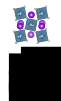
\includegraphics[width=\textwidth]{./data/plots/anharmonicity/2_materials/both.pdf}
	\caption{
		\label{fig:KCaF3}
		KCaF$_3$ in the low-temperature Pnma~(top) and high-temperature cubic phase~(bottom). Both structures are viewed along the long $b$-axis.
	}
	\label{fig:anh.KCaF3}
\end{marginfigure}

\newthought{Furthermore, it is instructive to evalute the anharmonicity for single configurations}, be it snapshots in time during molecular dynamics simulations, or when using other sampling approaches,~e.\,g,~harmonic Monte Carlo samples as defined in Eq.\,\eqref{eq:ha.samples}. While we will discuss ``time-resolved anharmonicity'' in detail at a later point, we show the evaluation of $\sigmaA$ for samples generated by Eq.\,\eqref{eq:ha.samples} in Fig.\,\ref{fig:anh.sampling}.
\begin{figure}
	\includegraphics[width=4.1in]{./data/plots/anharmonicity/7_sampling/convergence_sigma_MC.pdf}
	\caption{
			Anharmonicity measure $\sigmaA$ evaluated for individual atomic configurations obtained from Eq.\,\eqref{eq:ha.samples}. Dots: $\sigmaA [{\bf R}_n]$ for individual samples; Red line: Cumulative average.	Black dashed line: $\sigmaA$ from \emph{ai}MD.	Shadowed region: Convergence estimated by standard error.
	}
	\label{fig:anh.sampling}
\end{figure}
The analysis shows that a decent estimate of the anharmonicity measure $\sigmaA$ can be obtained from the harmonic sampling analysis with few samples, especially for silicon, where every individual harmonic sample yielded a $\sigmaA$ within 99\,\% of the reference value obtained by MD simulation for several hundred simulation time steps indicated by the dashed vertical line. For the more anharmonic KCaF$_3$, the harmonic sampling with 30~samples yields an estimated value of $\sigmaA_{\rm est.} = 0.38$, which differs from the MD value ($\sigmaA = 0.36$) by about 5\,\%. A distinction between largely harmonic materials like silicon, and anharmonic materials like KCaF$_3$ is therefore possible with very few samples

\newthought{Motivated by this fact, investigated the possiblity to estimate $\sigmaA$ based on a single samples}, as suggested by Zacharias and coworkers in Ref.\,\cite{Zacharias2016}, where a single, deterministic sample probing the most probable part of the harmonic distribution is used by using a fixed $\zeta_s = (-1)^s)$ instead of a random distribution in Eq.\,\eqref{eq:ha.samples}. We denote anharmonicity measures obtained by such a ``one-shot'' approach by $\sigmaAOS$ in the following. As shown in Fig.\,\ref{fig:anh.one-shot}, the one-shot samples provide very good estimates for silicon in the the entire temperature range from 200\,K to 800\,K, which can be expected due to the largely harmonic nature of silicon.
\begin{figure}
	\includegraphics[width=4.1in]{./data/plots/anharmonicity/7_sampling/sigma_temp_one_shot.pdf}
	\caption{
		$\sigmaA$ as a function of temperature obtained from MD~simulations (black circles) and one-shot sampling (triangles connected by dashed curves)
	}
	\label{fig:anh.one-shot}
\end{figure}
For KCaF$_3$, the agreement is good in the temperature range from 200\, to 400\,K, at least within the limits of the harmonic sampling approach as discussed in the previous paragraph, taking into account that only a single sample was used. Above 500\,K, however, the difference to the reference value from MD simulations increases, which is due to the phase transition occuring in KCaF$_3$ discussed earlier, which also occurs in the simulation cell. A prediction of anharmonicity across phase transitions can therefore not be expected, which can be expected by noting that the entire reference frame for the harmonic model changes when a phase transition occurs. The phase transition mechanism of KCaF$_3$ and implications for the anharmonicity measure are further discussed in Ref.\,\cite{Knoop2020}.

\newthought{Ultimately, the applicability of the one-shot sampling approach} needs to be assessed for a diverse set of materials, especially if one aims to use this scheme to screen for anharmonicity in material space. As shown in Fig.\,\ref{fig:anh.screening} for a set of 63~materials, the one-shot sampling is reliable within $\pm 10\,\%$ for all materials in the set up to a value of about $\sigmaA \simeq 0.3$.
\begin{figure}
	\includegraphics[width=4.1in]{./data/plots/anharmonicity/8_screening/sigma_os_md.pdf}
	\caption{
		Comparison of the anharmonicity measure obtained from MD simulations and one-shot sampling (OS) for 63 materials at 300\,K. The set comprises 25 rock salt (RS), 21 zincblende (ZS), 7 wurtzite (WZ), and 10 orthorombic perovskite (Perov.) materials. The diagonal line denotes perfect agreement between MD and OS, and the green area denotes a 10\,\%~error margin to guide the eye.
		Data was taken from Ref.\,\cite{Knoop2020}.
	}
	\label{fig:anh.screening}
\end{figure}
For larger values of $\sigmaA$, the deviation can become larger, especially for the rock salt materials with $\sigmaA \simeq 0.35$ which the one-shot sampling overestimates by about 20\,\%. Nevertheless, the agreement is qualitatively correct up to values of about $\sigmaA \simeq 0.5$, after which materials begin to show effects not captures by the harmonic sampling,~e.\,g.,~phase transition as discussed earlier for KCaF$_3$. In particular, the three highlighted noble metal halides AgBr, CuCl, and CuBr deviate strongly. These materials tend towards non-perturbative effects during the MD simulation such as spontaneous defect formation~\cite{Knoop2020}, which is a dynamical effect impossible to be described by any reference harmonic model. We will discuss the nature of these effects in more detail later. To conclude, we point out that also in the case of non-trivial dynamical effects such as defect formation, the estimated anharmonicity scored $\sigmaAOS$ are larger than $\gtrapprox 0.5$, and therefore indicate strong anharmonicity. Classifying strong anharmonicity in terms of one-shot sampling, $\sigmaAOS$, is therefore possible for all materials in the set.


\subsection{Anharmonicity and thermal conductivity}

Based on the qualitative discussion of thermal transport in Sec.\,\ref{sec:hf.kappa.ha}, one can expect that stronger anharmonicity leads to shorter phonon lifetimes and therefore lower thermal conductivity. We tested this hypothesis for a list of 47 materials where experimental reference was available~\cite{Morelli2006,Chen2019}. The results are shown in Fig.\,\ref{fig:anh.kappa}.
\begin{figure}
	\includegraphics[width=4.1in]{./data/plots/anharmonicity/9_kappa/sigma_vs_kappa.pdf}
	\caption{
		Experimental thermal conductivity at room temperature, $\kappa^{\rm exp}_{300\,{\rm K}}$, versus one-shot measure of anharmonicity, $\sigmaAOS$. The dashed diagonal line indicates a power law fit for the data. The grey area denotes values of $\kappa$ which agree with the fit within an order of magnitude. The dataset contains 47 materials, 22 rock salt (RS), 19 zincblende (ZB), and 6 wurtzite (WZ) structures. Experimental data from Ref.~\cite{Morelli2006,Chen2019}.
	}
	\label{fig:anh.kappa}
\end{figure}
The analysis reveals an inverse power law relationship between thermal conductivity and anharmonicity for the materials in the dataset. Given that just a single descriptor was used,~i.\,e.,~the estimated anharmonicity score, and not further vibrational properties as commonly employed in semi-empirical models for thermal condcutivity\CITE{Curtarolo,Toberer,Ramprasad}, this observation is too some extent surprising, although encouraging that $\sigmaA$ captures some essential physics relevant to heat transport.

\newthought{The most important messages from Fig.\,\ref{fig:anh.kappa} can be summarized as follows}:
\begin{enumerate}
	\item Largely harmonic materials with $\sigmaA \simeq 0.1$, like diamond (C), boron nitride (BN), or boron phosphide (BP) can be expected to be good thermal conductors with $\kappa \gtrsim 100\,{\rm W/mK}$.
	\item Strongly anharmonic materials with $\sigmaA \gtrsim 0.3$ can be expected to be poor thermal conductors with $\kappa \lesssim 10\,{\rm W/mK}$, if one adopts the definition suggested by Morelli and Slack to define ``high thermal conductivity'' as $\kappa \gtrsim 50 \, {\rm W/mK}$~\cite{Morelli2006}.
	\item $\sigmaA$ has a strong correlation with thermal conductivity across the entire dataset, but nevertheless only a rough estimate can be made, especially in the middle region with $\sigmaA \simeq 0.2$. This can be best seen by comparing strontium oxide (SrO) with $\kappa = 10\,{\rm W/mK}$ and $\sigmaA = 0.22$, and zinc oxide (ZnO) with $\kappa = 60\,{\rm W/mK}$ and $\sigmaA = 0.24$, or beryllium oxide (BeO) with $\kappa = 370\,{\rm W/mK}$ and $\sigmaA = 0.16$ to magnesium oxide (MgO) with $\kappa = 60\,{\rm W/mK}$ and $\sigmaA = 0.18$. These pairs of materials differ only slightly in their estimated anharmonicity, but still quite strongly in the thermal conductivity. 
\end{enumerate}

\newthought{These findings suggest the following approach} towards screening material space in search for thermal insulators: Estimate the anharmonicity for materials of interest and discard the largely harmonic ones, as they will be good thermal conductors most of the time. Of course, the reverse approach can be pursued when searching for materials with potentially high thermal conductivity.

\subsection{Candidate Materials}
In the context of the work published in Ref.\,\cite{Knoop2020}, we have identified a set of 


% \part{Benchmarks?}

% \part{Results}
\chapter{Screening Materials for Anharmonicity}
\section{Screening Material Space}

\subsection{Preparation: Efficient Sampling of Anharmonicity}

\begin{figure}
	\includegraphics[width=4.1in]{./plots/anharmonicity/7_sampling/convergence_sigma_MC.pdf}
	\caption{
		Some text to describe the figure.
	}
\end{figure}

\begin{figure}
	\includegraphics[width=4.1in]{./plots/anharmonicity/7_sampling/sigma_temp_one_shot.pdf}
	\caption{
		Some text to describe the figure.
	}
\end{figure}

\begin{figure}
	\includegraphics[width=4.1in]{./plots/anharmonicity/8_screening/sigma_os_md.pdf}
	\caption{
		Some text to describe the figure.
	}
\end{figure}

\subsection{Literature Review}
Lorem ipsum dolor sit amet, consetetur sadipscing elitr, sed diam nonumy eirmod tempor invidunt ut labore et dolore magna aliquyam erat, sed diam voluptua. At vero eos et accusam et justo duo dolores et ea rebum. Stet clita kasd gubergren, no sea takimata sanctus est Lorem ipsum dolor sit amet. Lorem ipsum dolor sit amet, consetetur sadipscing elitr, sed diam nonumy eirmod tempor invidunt ut labore et dolore magna aliquyam erat, sed diam voluptua. At vero eos et accusam et justo duo dolores et ea rebum. Stet clita kasd gubergren, no sea takimata sanctus est Lorem ipsum dolor sit amet.

\begin{figure}
	\includegraphics[width=4.1in]{./plots/anharmonicity/9_kappa/sigma_vs_kappa.pdf}
	\caption{
		Some text to describe the figure.
	}
\end{figure}

Lorem ipsum dolor sit amet, consetetur sadipscing elitr, sed diam nonumy eirmod tempor invidunt ut labore et dolore magna aliquyam erat, sed diam voluptua. At vero eos et accusam et justo duo dolores et ea rebum. Stet clita kasd gubergren, no sea takimata sanctus est Lorem ipsum dolor sit amet. Lorem ipsum dolor sit amet, consetetur sadipscing elitr, sed diam nonumy eirmod tempor invidunt ut labore et dolore magna aliquyam erat, sed diam voluptua. At vero eos et accusam et justo duo dolores et ea rebum. Stet clita kasd gubergren, no sea takimata sanctus est Lorem ipsum dolor sit amet.

\subsection{Candidate Materials}

\chapter{Thermal Conductivities for Strongly Anharmonic Compounds}
\section{Overview: Results of Dataset}
\section{Discussion}
\subsection{Comparision to Experiment}

\begin{figure}
	\includegraphics[width=\textwidth]{./data/plots/kappa_vs_exp/kappa_vs_exp.pdf}
	\caption{Comparison to experiment. Bullets($\bullet$): Single crystal. Stars ($\star$): Polycrystalline or thin-film experiment. Error bar in y-directioin: Statistical uncertainty for $\kappa^{\rm aiGK}$ from standard error over individual trajectories and Cartesian components~[ref]. Green band: Agreement between mean experiment and mean computation with $\pm 15\,\%$ deviation.}
	\label{fig:kappa_exp}
\end{figure}

\subsection{Relation to Anharmonicity}

\begin{figure}
	\includegraphics[width=\textwidth]{./data/plots/kappa_vs_sigma/kappa_vs_sigma.pdf}
	\caption{Thermal conductivity at room temperature vs. anharmonicity measure.}
	\label{fig:kappa_sigma}
\end{figure}

\section{Dynamical Effects}

\subsection{CuI}

\begin{figure}
	\includegraphics[width=\textwidth]{./data/plots/defects/216.02.CuI/sigma_vs_time.pdf}
	\caption{Zincblende (SG\,216) CuI, describe}
	\label{}
\end{figure}

\begin{figure*}
	\includegraphics[width=.5\textwidth]{./data/plots/defects/216.02.CuI/perfect_110_solid.png} \hfill
	\includegraphics[width=.5\textwidth]{./data/plots/defects/216.02.CuI/defect_110.png}
	\caption{CuI viewed in (110) direction. Left: High-symmetry zincblende structure. Right: Copper ion in lower-right quadrant moves into interstitial site along (111) direction.}
	\label{}
\end{figure*}

\begin{figure*}
	\includegraphics[width=.5\textwidth]{./data/plots/defects/216.02.CuI/defects_110.png} \hfill
	\includegraphics[width=.5\textwidth]{./data/plots/defects/216.02.CuI/defects_110_135.png}
	\caption{2.5 defects in (110) and rotated by 90\,deg about z-axis.}
	\label{}
\end{figure*}

\subsection{KCaF$_3$}

\begin{figure}
	\includegraphics[width=\textwidth]{./data/plots/defects/062.05.KCaF3/sigma_vs_time.pdf}
	\caption{Orthorombic (SG\,62) KCaF$_3$, describe}
	\label{}
\end{figure}

\begin{figure*}
	\includegraphics[width=.5\textwidth]{./data/plots/defects/062.05.KCaF3/plots/ref_front.png} \hfill
	\includegraphics[width=.5\textwidth]{./data/plots/defects/062.05.KCaF3/plots/2_front.png} \\
	\includegraphics[width=.5\textwidth]{./data/plots/defects/062.05.KCaF3/plots/4_front.png} \hfill
	\includegraphics[width=.5\textwidth]{./data/plots/defects/062.05.KCaF3/plots/5_front.png}
	\caption{Front view along long axis.}
	\label{}
\end{figure*}

\begin{figure*}
	\includegraphics[width=.5\textwidth]{./data/plots/defects/062.05.KCaF3/plots/ref_left.png} \hfill
	\includegraphics[width=.5\textwidth]{./data/plots/defects/062.05.KCaF3/plots/2_left.png} \\
	\includegraphics[width=.5\textwidth]{./data/plots/defects/062.05.KCaF3/plots/4_left.png} \hfill
	\includegraphics[width=.5\textwidth]{./data/plots/defects/062.05.KCaF3/plots/5_left.png}
	\caption{Left view along short axis.}
	\label{}
\end{figure*}

\begin{figure}
	\includegraphics[width=\textwidth]{./data/plots/defects/062.05.KCaF3/rdf/geometry_in_def_4.pdf}
	\caption{RDF trajectory 4}
	\label{}
\end{figure}

\chapter{Conclusion}

\chapter{Outlook}




% \setcounter{secnumdepth}{-1}

% part*{appendix}

% \setcounter{tocdepth}{1}
% \addtocontents{toc}{\setcounter{tocdepth}{0}}
\addtocontents{toc}{\protect\setcounter{tocdepth}{0}}
\begin{appendices}
%  \appendixpage
  \part*{Appendix}
  \chapter{Notation}
\label{app:notation}
\epigraph{\singlespacing \it ``It is useful to start by declaring one's notations.''}{Paul Gartner}

\section{Indexation}
Throughout the thesis, we use the following symbols to index and label the appearing quantities:
\begin{itemize}
\item $\alpha, \beta, \gamma, \delta$: Cartesian component indices,
\item $\mu, \nu, \rho$: crystal-basis component indices,
\item $I, J$: atom number labels,
\item $i, j$: atom labels in the primitive cell,
\item ${\bf L}, {\bf K}$: lattice vectors.
\end{itemize}
We use a contra/covariant notation for vector components following Sands~\cite{Sands2002}, with an Einstein convention,
$$
{\bf x} \cdot {\bf y} = \sum_\alpha x^\alpha y_\alpha \equiv x^\alpha y_\alpha~,
$$
for sums over vector components. In particular, we have
\begin{itemize}
	\item ${\bf R}_I = (R^1_I, R^2_I, R^3_I)$: Atomic position of atom $I$ in a Cartesian components.
	\item $\set{{\bf a}_\mu}$: crystal basis with lattice vectors ${\bf a}_\mu$.
	\item $\set{{\bf a}^\mu}$: dual basis with inverse lattice vectors ${\bf a}^\mu$ fulfilling ${\bf a}^\mu \cdot {\bf a}_\nu = \delta^\mu_{~\nu}$. The cartesian components of $\set{{\bf a}^\mu}$ and $\set{{\bf a}_\mu}$ are related by
	$$ a^{\mu}_{~\alpha} = (\itp a)_{\mu \alpha} ~.$$
	\item ${\bf R}_I = R^\mu_I {\bf a}_\mu$: Atomic position of atom $I$ expressed in the crystal basis $\set{{\bf a}_\mu}$. The are $R_I^\mu$ are also called \emph{scaled} or \emph{fractional} components. They are related to the Cartesian components $R_I^\alpha$ by $R_I^\mu = {\bf a}^\mu \cdot {\bf R}_I = (\itp a)_{\mu \alpha} R_I^{\alpha}$ by the identity stated above.
	\item ${\bf L} = L^\mu {\bf a}_\mu$: A lattice vector $\bf L$ expressed in the crystal basis $\set{{\bf a}_\mu}$. 
	\item $\set{{\bf b}^\mu}$: reciprocal lattice vectors fulfilling ${\bf b}^\mu \cdot {\bf a}_\nu = 2 \pi \delta^\mu_{~\nu}$,~i.\,e.,~${\bf b}^\mu = 2\pi\,{\bf a}^\mu$ with the crystallographic convention of including the factor $2 \pi$ in the basis defintion.
	\item ${\bf q} = q_\mu {\bf b}^\mu$: phonon wave vector in the reciprocal lattice basis $\set{{\bf b}^\mu}$.
	\item ${\bf q} \cdot {\bf R}_I = 2 \pi \, q_\mu R^\mu_I$: scalar product of wave vector with atomic position.
\end{itemize}
We remind the reader that in Cartesian space, indices can be lowered and raised arbitrarily,~i.\,e.,~the components $x^\alpha$ and $x_\alpha$ are equal.

\chapter{Bloch Theorem and Brillouin Zone}
\epigraph{\singlespacing \it ``The idea of periodicity in the reciprocal space is useless but, I think, harmless.''}{Paul Gartner}
\section{Bloch Theorem}
\label{sec:BlochTheorem}
The Schr\"odinger equation in 1d reads
\begin{align}
	\hat H \psi (x) = \left( - \frac{\nabla^2}{2m} + V(x) \right) \psi (x) = E \psi (x)~.
	\label{eq:app.bloch.se}
\end{align}
In a periodic potential,
\begin{align}
	V(x + a) = V(x)~,
	\label{eq:app.bloch.potential}
\end{align}
the periodicity can be expressed by stating that the translation operator $\hat T_a$ defined by its action,
\begin{align}
	\hat T_a f(x) = f(x + a)~,
	\label{eq:app.bloch.Ta}
\end{align}
commutes with the Hamiltonian,
\begin{align}
	\left[ \hat H , \hat T_a\right] = 0~.
	\label{eq:app.bloch.commute}
\end{align}
The eigenstates $\psi (x)$ of $\hat H$ are therefore also eigenstates of $\hat T_a$~\cite{Basdevant2000}. The translation operator is unitary, $\D{\hat T}_a = \hat{T}_a^{-1}$, but not hermitian. The eigenvalues $\lambda$ associated with $\hat T_a$ are thus complex numbers. By definition, one has \mbox{$\psi ( x + na ) = \lambda^n \psi(x)$}. Requiring bounded solutions, $\lim_{x \rightarrow \infty} \lvert \psi (x) \rvert < \infty$, imposes the condition $\lvert \lambda \rvert = 1$.
The function $\psi$ can therefore be written as
\begin{align}
	\psi (x) = c(x) u(x)~,
\end{align}
with a real, periodic function
\begin{align}
	u: \mathds R \rightarrow \mathds R
	\quad\text{with}\quad u(x + a) = u(x)~,
\end{align}
and a complex function of unit modulus,
\begin{align}
	c: \mathds R \rightarrow \mathds C
	\quad\text{with}\quad \left\lvert c(x) \right\rvert = 1~.
	\label{eq:app.bloch.c1}
\end{align}
We label each possible solution by the number $k$, then
\begin{align}
	c_k (x) = {\rm e}^{\im k x}
	%% don't impose uniqeness here
	%\quad\text{with}\quad k \in \left[0, \frac{2 \pi}{a} \right)
	\label{eq:app.bloch.c2}
\end{align}
% is a unique map from the domain $x \in [0, a)$ to the complex unit circle $\set{z \in \mathds C : \lvert z \rvert = 1}$. 
is a map from the domain $x \in \mathds R$ to the complex unit circle $\set{z \in \mathds C : \lvert z \rvert = 1}$. 
It then holds that $\hat T_a \psi_k (x) = {\rm e}^{\im k a} \psi(x)$,~i.\,e.,~$\psi_k$ is an eigenfunction of $\hat T_a$ with eigenvalue $\lambda = {\rm e}^{\im k a}$. We formulate the
\begin{thm}[Bloch]
	Solutions to the Schr\"odinger equation~\eqref{eq:app.bloch.se} with a periodic potential of periodicity $a$ are of the form
	\begin{align*}
		\psi_k (x) = {\rm e}^{\im k x} u_k (x)~,
	\end{align*}
	with a real, periodic function $u_k$.
%	 for each $k$ in the first Brillouin zone,
%	\begin{align*}
%		k \in \left[0, \frac{2 \pi}{a} \right)~.
%	\end{align*}
\end{thm}
The theorem is trivially extended to the 3d case by using the multiplication rule
\begin{align}
	\hat{T}_{{\bf a} + {\bf b}} f({\bf x}) = \hat{T}_{\bf a} \hat{T}_{\bf b} f({\bf x}) \equiv f({\bf x} + {\bf a} + {\bf b})~.
\end{align}
A more rigorous proof in terms of representation theory can be found,~e.\,g.,~in~\cite{Dresselhaus2007}.

\section{Brillouin Zone}
\label{sec:BrillouinZone}
We have not yet specified the range of the quantum number $k$. This can be done by requiring the complex function $c_k$ defined in Eq.\,\eqref{eq:app.bloch.c2} to map the interval $x \in [0, a)$ \emph{exactly once} to the unit circle so that $k$ is a \emph{unique} label for the eigenvalues ${\rm e}^{\im k a}$ of the translation operator $\hat T_a$.
We therefore define the
\begin{align}
	\text{Brillouin zone} = \set{k : k \in \left[ - \frac{\pi}{a}, \frac{\pi}{a}\right)}~.
\end{align}
For a wavefunction belonging to $k' = k + G$, where $G$ is an integer multiple of the the reciprocal lattice vector $b = 2\pi / a$, we would find
\begin{align}
	\hat T_a \psi_{k + G} (x) = {\rm e}^{\im k a} \psi_{k + G} (x)~.
\end{align}
They are therefore indistinguishable by the translation operator and we define $\psi_k$ and $\psi_{k+G}$ to be the same function,
\begin{align}
	\psi_k (x) = \psi_{k + G} (x)~.
\end{align}
This is sometimes termed ``periodicity of Bloch functions in reciprocal space''.

\chapter{Born-von Karman Supercell}
To ensure normalizability of the functions $\psi_{{\bf k}l}$, one additionally imposes the \emph{Born-von Karman boundary conditions}
\begin{align}
\psi_{{\bf k}l} ({\bf x} + {\bf A}_i) 
= \psi_{{\bf k}l} ({\bf x})
%\label{eq:dft.Bloch.4}
\end{align}
where each ${\bf A}_i$ is a linear combination of the primitive basis vectors $\set{{\bf a}_i}$,
\begin{align}
{\bf A}_i = S_i^{~j} {\bf a}_j\quad\text{with } S_i^{~j} \in \mathds Z~,
\end{align}
where $S$ is a non-singular matrix with integer elements. The space spanned by the $\set{{\bf A}_i}$ is parallelepiped of volume $V = N \, {\bf a}_1 \cdot ({\bf a}_2 \times {\bf a}_3)$, where $N = \det S$ is the number of unit cells that fit into the enlarged cell. This cell is therefore often called \emph{supercell}, and the matrix $S$ is denoted as a \emph{supercell matrix}.
With the Born-von Karman boundary conditions, the domain of all functions and functionals appearing in the Kohn-Sham equations become restricted to the supercell. The ideal, infinite crystal is obtained in the limit $N \rightarrow \infty$.
Using the periodic boundary condition expressed by Eq.\,\eqref{eq:dft.Bloch.4} in the Bloch functions given by Eq.\,\eqref{eq:dft.Bloch.2}, and the periodicity of the functions $u_{{\bf k} l}$, one finds that
\begin{align}
%	{\rm e}^{\im {\bf k} \cdot ({\bf x} + N_i {\bf a}_i)} u_{{\bf k} l} ({\bf x})
%		&= {\rm e}^{\im {\bf k} \cdot {\bf x}} u_{{\bf k} l} ({\bf x}) \nonumber \\
%	\implies
%		{\rm e}^{\im {\bf k} \cdot  N_i {\bf a}_i} 
%			&= 1 \nonumber \\
%	\implies
{\bf k} \cdot {\bf A}_i
&= 2 \pi m_i\quad\text{with } m_i \in \mathds N \text{ such that } 
\forall i: {\bf k} \cdot {\bf a}_i \leq 2 \pi~.
%\label{eq:dft.Bloch.5}
\end{align}
In total there are $N$ permissible values of $\bf k$ labelled by ${\bf m} = (m_1, m_2, m_3)$ that can be expressed in terms of the \emph{reciprocal lattice vectors}~\cite{Sands2002}
\begin{align}
{\bf B}^i 
= 2 \pi \varepsilon^{ijk} \frac{{\bf A}_j \times {\bf A}_k}{{\bf A}_1 \cdot ({\bf A}_2 \times {\bf A}_3)} ~,
%\label{eq:dft.Bloch.bi}
\end{align}
where $\varepsilon^{ijk}$ denotes the Levi-Civita symbol enforcing the correct ordering of $ijk$. The complete set of $\bf k$-values is
\begin{align}
{\bf k}_{\bf m} 
= \sum_{i=1}^3 m_i {\bf B}^i~.
%\label{eq:dft.Bloch.k_m}
\end{align}
The values of $\bf k$ given by Eq.\,\eqref{eq:dft.Bloch.k_m} are those sampled in real-space simulation in a box of the given size,~i.\,e.,~the \emph{Born-von Karman cell}.

\chapter{Numerical Force Constants}
\label{app:force_constants}
The force constants $\Phi$ can be obtained from first-order derivatives of the potential-energy surface,~i.\,e.,~the forces, by rewriting the second derivative in terms of a finite difference expression,
\begin{align}
\Phi_{I \alpha, J \beta}
= \left.\frac{\partial^{2} \mathcal{V}(\mathbf{R})}{\partial R_{I}^{\alpha} \partial R_{J}^{\beta}}\right|_{\mathbf{R}^{0}}
= - \frac{\partial}{\partial R_I^\alpha} F_{J, \beta}
= - \lim_{\epsilon \to 0}
\frac{F_{J, \beta} (\set{\b R': R^{\prime \alpha}_I = R^{0, \alpha}_I + \epsilon )}}{\epsilon}
~.
\label{eq:FC2_finite}
\end{align}
In practice, atom $I$ is displaced by a small but finite displacement $\epsilon$ in the direction $\alpha$, and the force on all other atoms is recorded. By performing the displacement in all $3N$ degrees of freedom, the $3N \times 3N$ forces can be arranged in a matrix ${\rm F}_{[3N \times 3N]}$, and the displacements can be arranged in a matrix ${\rm U}_{[3N \times 3N]} = \epsilon \mathds 1_{[3N \times 3N]}$. The $3N \times 3N$ force-constants matrix $\Phi$ is obtained by the trivial matrix multiplication
\begin{align}
{\rm F }
&= - \Phi {\rm U} 
= - \epsilon \Phi \mathds 1
\label{eq:finite.diff.1}
\\
\implies
\Phi &= - \frac{1}{\epsilon} {\rm F} \mathds 1~.
\end{align}
%\begin{align}
%	F &= - H U \\
%	\implies
%	H &= - U^{+} F \\
%	F &= \begin{pmatrix} \b F_1, & \cdots, & \b F_{3N} \end{pmatrix}
%\end{align}
If $M > 3N$ displacements are used,~e.\,g.,~because positive and negative displacements $\pm \epsilon$ are used, the force constants can be obtained by solving an overdetermined linear equation of the kind
\begin{align}
{\rm F}_{[3N \times M]} &= - \Phi_{[3N \times 3N]} {\rm U}_{[3N \times M]} \\
\implies
\Phi &= - {\rm F} {\rm U}^{+}~,
\label{eq:phi.pseudo.1}
\end{align}
where ${\rm U}^{+}$ denotes the Moore-Penrose pseudo inverse of the displacement matrix $\rm U$~\cite{Penrose1955,Parlinski1997}.

\newthought{The number of required force calculations} can be reduced by considering the spacegroup symmetry of the crystal. This can be achieved in two ways: First, the symmetry can be used to identify the set of inequivalent displacements from which all other forces can be constructed by the following argument: We define the representation $\Gamma^g$ of a symmetry operation $g$ by its action on the atomic coordinates $\set{\b R_I = \b R_I^0 + \b U_I}$ as
\begin{align}
\b R_I^{g} &\equiv {\Gamma}^g (\b R_I) = { P}^g_{IJ} \b R^0_J + { M}^g \b U_I~,
\label{eq:sym.RI'}
\end{align}	
where $P^g_{IJ}$ is the permutation that relates the reference positions of atom $I$ and atom $J$, and $M^g$ is an orthogonal matrix representing the rotation (or inversion) of the respective displacement.\begin{marginfigure}
	\centering
	\includegraphics[width=\textwidth]{./data/sketches/symop.jpg}
	\caption{The configurations $\b R$, $\b R^g$, and $\tilde{\b R}^g$ obtained from the symmetry operation $g=\text{90 degrees rotation}$ for a two-dimensional system with five atoms. Arrows indicate the force at each atom.}
	\label{fig:symmetry.1}
\end{marginfigure}
\newthought{As depicted in Fig.~\ref{fig:symmetry.1}}, the forces on each atom in the rotated system $\b R^g = \set{\b R^g_I}$ are obtained by co-rotating the forces in the initial configuration $\b R = \set{\b R_I}$ as
\begin{align}
\b F_I (\b R^g) &= {M}^g \b F_I (\b R)~,
\label{eq:sym.Fp}
\end{align}
i.\,e.,~the forces transform as the displacements $\b U_I$.
Let us now define a new configuration $\tilde{\b R}^g$ where just the displacements $\b U_I$ are rotated according to $g$. This can be achieved by rotating the entire system according Eq.\,\eqref{eq:sym.RI'} and applying the inverse permutation $P^{g-1}$,~i.\,e.,
\begin{align}
\tilde{\b R}_I^g 
&= P^{g-1}_{IJ} \b R_I^g 
\stackrel{\eqref{eq:sym.RI'}}{=} \b R^0_I + {\rm M}^g P^{g-1}_{IJ} \b U_J~.
\end{align}
It follows that the force on atom $I$ in the new configuration $\tilde{\b R}^g$ is related to the force in the rotated system $\b R^g$ by this inverse permutation, so that
\begin{align}
\b F_I (\tilde{\b R}^g) 
&= {P}^{g-1}_{IJ} \b F_J (\b R^g) 
= {M}^g  {P}^{g-1}_{IJ} \b F_J (\b R)~.
\label{eq:sym.Ftilde}
\end{align}
By means of this equation, the set of forces obtained for a configuration $\set{\b R_I = \b R_I^0 + \b U_I}$ can be used to generate a set of forces for each symmetrically equivalent configuration $\set{\tilde{\b R}_I^g = \b R_I^0 + {\rm M}^g P^{g-1}_{IJ} \b U_J}$, where $g$ are spacegroup elements.

A complementary approach is to use the symmetry elements $\set{g}$ to reduce the forceconstant matrix to an irreducible basis,
\begin{align}
\Phi 
= \sum_{i=1}^{D} p_i \tilde{\Phi}_i~,
\label{eq:sym.Phi.irrep.1}
\end{align}
where the $\tilde{\Phi}_i$ are \emph{solely} determined by the space group elements $\set{g}$ and analytical properties of the forceconstants, and only the \emph{irreducible components} $p_i$ are system dependent. The pseudoinverse procedure given in Eq.\,\eqref{eq:phi.pseudo.1} then only has to be performed for the $D$ parameters $p_i$~\cite{Parlinski1997}. This procedure can drastically reduce the number of free parameters in the forceconstant matrix. For example, in a $4\times4\times4$ bcc lattice with 128 atoms, $\Phi$ is a matrix with $(3 \cdot 128)^2 = 147456$ elements. However, there are only $D=11$ irreducible parameters $p_i$ that need to be determined~\cite{Hellman2013}.

\TODO{Add the theory for symmetry reduction}

\section{Temperature Dependent Effective Potentials}
\TODO{Add TDEP}

\chapter{Geometry Optimization for Crystals}
\section{Lattice optimization at zero temperature}
\label{sec:ltrm}
The task of geometry optimization is to find a local minimum $\b R^0$ of the potential-energy surface $\mathcal{V} (\b R)$. From a mathematical point of view, $\mathcal V (\b R)$ is a function of the $3N$ coordinates $\b R$, or, when lattice degrees of freedom are included, $3N + 9$ degrees of freedom.\footnote{When rotations are rigorously excluded, the lattice only has 6~degrees of freedom.} Summarizing the positional degrees of freedom including the lattice in the generalized coordinate
\begin{align}
x 
= \left( R_{0}^x, R_{0}^y, \ldots, R_{N}^z; a^x_{~1}, a^x_{~2}, \ldots, a^z_{~3} \right) ~,
\label{eq:opt.x}
\end{align}
we seek to find
\begin{align}
x^0 = \arg \min_x \mathcal V (x)~.
\end{align}
The standard tools to solve this problem are very well covered in the standard reference~\cite{nocedal2006}. The technical pitfalls when optimizing lattices are thoroughly discussed in~\cite{pfrommer1997,Tadmor1999}.
A slightly different approach as the ones discussed in the references listed above is taken in the molecular simulations code \textsc{FHI-aims}~\cite{FHI-aims}. We therefore review this approach shortly in the following.

\newthought{Many optimization algorithms} working with gradients as input are based on the Newton descent method in which the target function is locally approximated by a second-order Taylor expansion~\cite{nocedal2006}. In our case, we denote the generalized force as $f_x$ and the Hessian matrix of second derivatives as ${\rm H}_{xx'}$, where
\begin{align}
f_x 
&= - \partial_x \mathcal V (x)~,
\label{eq:opt.f} \\
{\rm H}_{xx'} 
&= \partial_x \partial_{x'} \mathcal{V} (x)~.
\label{eq:opt.H}
\end{align}
Assuming that $f_x$ and ${\rm H}_{xx'}$ are known, the neighborhood of a configuration $x$ can be written to second order in a displacement $s_x$ as\marginnote{Sum convention \mbox{$s_x f_x \equiv \sum_x s_x f_x$} is implied.}
\begin{align}
m(x + s_x) 
= \mathcal V (x) - s_x f_x + \halb \fD s_x \fD {\rm H}_{xx'} \fP s_{x'}~.
\label{eq:opt.m}
\end{align}
The minimum of this function is given by
\begin{align}
s_x = {\rm H}_{xx'}^{-1} \fD f_{x'}~,
\end{align}
which is the essence of the Newton method. One beneficial property of the Newton method is that the exact Hessian $\rm H$ is not required to be known, and one can find approximate matrices $\rm B$ that yield good results. Replacing the exact $\rm H$ by an approximate matrix $\rm B$ is known as the \emph{quasi}-Newton method.
Typically, an initial approximate Hessian $\rm B^0$ is chosen to be of simple form,~e.\,g.,~a constant times unit matrix, or based on some simpler model~\cite{lindh1995}. The initial guess is then updated during the optimization, for example by means of the  Broyden–Fletcher–Goldfarb–Shanno (BFGS) algorithm.\footnote{BFGS update for the estimated Hessian $B^i$ from step $i$ to $i+1$:
	\begin{align*}
	{\rm B}^{i + 1}_{xx'}
	= {\rm B}^i_{xx'} 
	& + \frac{{\rm B}^i_{x\fP{y}} s^i_{\fP{y}} s^i_{y'} {\rm B}^i_{y'x'} }{s^i_{\fP y} {\rm B}^i_{yy'} s^i_{y'}}
	- \frac{\delta f^i_{\fP x} \delta f^i_{x'}}{\delta f^i_{\fP x} s^i_{x'}}~,
	\end{align*}
	with $\delta f^i = f^{i+1} - f^i$.
}
The configuration $x$ is updated according
\begin{align}
x^{i+1} = x^i + s_x^i = ~x^i + {\rm B}^i_{xx'} f^i_{x'}.
\end{align}

\newthought{If the lattice degrees of freedom} are represented by the Cartesian components $a^\alpha_i$ of the lattice vectors, the generalized force on the lattice is given by\marginnote{Symbolically:
	$$
	f_a 
	= -\frac{\partial \mathcal V}{\partial a} 
	= -V \underset{\fD \sigma}{\underbrace{\frac{1}{V}\frac{\partial \mathcal V}{\partial \varepsilon}}} \underset{\itp a}{\underbrace{\frac{\partial \varepsilon}{\partial a}}}~.
	$$
}
\begin{align}
f_a = - V \sigma \itp{a}~,
\end{align}
where $V = \det a$ is the unit cell volume, $\sigma$ is the $3 \times 3$~stress tensor, and $a$ is the lattice matrix.\footnote[][0em]{The lattice matrix is the collection of lattice vectors $\set{\b a_i}$,
	\begin{align}
	a = \begin{pmatrix} \b a_1, \b a_2, \b a_3 \end{pmatrix}~.
	\end{align}
}
For non-cubic systems, a diagonal Hessian matrix $B^0 = c \mathds 1$ will therefore produce steps proportional to the reciprocal cell $\itp{a}$ which, among other things, can break the space-group symmetry of the crystal. This behavior can be avoided by defining the initial Hessian as
\begin{align}
B^0 = c \itp{a} a^{-1}~,
\label{eq:opt.B0.new}
\end{align}
where $c$ is a numerical constant. This particular choice of $B^0$ can be viewed as making the Hessian diagonal in the native coordinate system of the lattice,~i.\,e.,~when deformations of the lattice are viewed as strain transformations in terms of the strain tensor $\varepsilon$. By the choice of the Hessian according to Eq.\,\eqref{eq:opt.B0.new}, the resulting steps $s^i_a$ will mimic such strain transformations early during the optimization:
\begin{align}
a^{i + 1} = a^i + s_a^i = (\mathds 1 + \varepsilon_s^i) a^i~.
\end{align}
Another detail that must be taken into account is that updates of the lattice necessarily have to keep the relative atomic positions expressed in the crystal basis,~i.\,e.,~their fractional coordinates, unchanged. The ideas outlined in this section have been implemented in~\textsc{FHI-aims} and the performance compared to the previous implementation is shown in Fig.\,\ref{fig:ltrm}.
\begin{marginfigure}
	\includegraphics[width=\textwidth]{./data/plots/relaxation/ltrm.pdf}
	\caption{Residual force component as function of the relaxation steps, before (\texttt{trm\_2012}) and after (\texttt{trm}) optimizing the relaxation routine in \textsc{FHI-aims} according to the considerations presented in this chapter.}
	\label{fig:ltrm}
\end{marginfigure}
The non-systematic decrease of the residual force observed in the previous implementation (\texttt{trm\_2012}) was due to spurious distortions of the lattice and dislocations of the atomic arrangements generated by keeping their \emph{Cartesian} instead of \emph{fractional} positions unchanged during the lattice update. These artifacts are absent in the updated implementation (\texttt{trm}). The force convergence is generally faster and better behaved.


\section{Lattice optimization at finite temperature: Lattice expansion}
At finite temperatures,\marginnote{The volume expansion is usually measured in terms of the \emph{thermal expansion coefficient} $\alpha (T)$~\cite{Kittel1969}
	\begin{align}
	\alpha (T) = \frac{1}{3 V} \frac{\partial V (T)}{\partial T}~.
	\label{eq:lattice.expansion.coefficient}
	\end{align}
}
the nuclear motion results in dynamical pressure $p(T)$ and the lattice reacts by deforming,
\begin{align}
a (T) = \bm ( \mathds 1 + \varepsilon (T) \bm ) a_0~,
\label{eq:lattice.T}
\end{align}
where $a_0$ is the 0\,K static lattice matrix, and $a (T)$ is the lattice at finite temperature given in terms of a \emph{strain transformation} $\varepsilon (T)$. 
The energy change per unit volume $\d W$ of a system subject to an infinitesimal strain deformation $\varepsilon$ is defined as
\begin{align}
\d W = \sigma_{\alpha}^{~\beta} \d \varepsilon^{\alpha}_{~\beta}~,
\label{eq:stress.strain}
\end{align}
where $\sigma$ is the \emph{stress tensor} of the system. The lattice $a(T)$ in thermal equilibrium will therefore be the lattice that minimizes the stress $\sigma$ in Eq.\,\eqref{eq:stress.strain}. Depending on the crystal symmetry~\cite{Nye1985}, the strain tensor $\varepsilon$ has up to six independent values. Equation\,\eqref{eq:stress.strain} therefore poses a six-dimensional optimization problem at a given temperature~$T$ which can be solved for example by coupling the system to a barostat and performing an $NPT$ simulation~\CITE{NPT}. In the language of the previous chapter, the lattice $a(T)$ is then given as a time or ensemble average $\braket{a}_{(p, T)}$ at thermodynamic conditions $(p, T)$. In practice however, this approach is quite inefficient and suffers from large noise, especially in the system sizes typically available to \emph{ab initio} MD simulations~\CITE{ai NPT}.

\newthought{An approximate solution} to the six-dimensional optimization problem of finding the finite temperature lattice $a (T)$ can be  found by the following rationale: We assume that the thermodynamic pressure at a given volume $V$ and temperature $T$ is given as
\begin{align}
p (V, T) \approx \frac{N k_{\rm B} T}{V} + p_{\rm pot} (V_0, T) + p_{\rm int}(V)~,
\label{eq:eos.p}
\end{align}
where $p_{\rm kin} (T) = N k_{\rm B} T / V$ is the kinetic pressure, and $p_{\rm pot} (V_0, T)$ is the potential part of the pressure in the system at reference volume $V_0$ which stems from the nuclear interaction $\mathcal V (\b R)$~\cite{Hansen1990}. The last term, $p_{\rm int} (V)$, is an internal pressure induced by the volume change. We assume that $p_{\rm int} (V)$ mainly stems from the lattice and is not temperature dependent. It can therefore be obtained from an equation of state parametrized at 0\,K, for example the \emph{Vinet equation}~\cite{Vinet1987}:
\begin{align}
p_{\rm int} (V) 
&= \frac{3 B_0}{X^2} (1-X) {\rm e}^{\eta (1-X)} \label{eq:p.Vinet} \quad\text{with} \\ 
X &= \left[\frac{V}{V_0}\right]^{\frac{1}{3}}
\quad\text{and}\quad
\eta 
= \frac{3}{2} \left(B_0' - 1 \right)~,
\end{align}
where $V_0$ is the volume, $B_0$ is the bulk modulus, and $B_0' = \partial B_0 / \partial p$ is the isothermal pressure derivative of the bulk modulus. All these three parameters are obtained for the static lattice and we neglect their temperature dependence. Once the full parametrization of Eq.\,\eqref{eq:eos.p} is known, the temperature-dependent volume $V_{\rm min} (T)$ is found by requiring zero pressure. The resulting pressure $p_{\rm int} (V_{\rm min})$ can be used to find the static reference lattice $a(T)$ by optimizing the geometry while applying the external pressure $p_{\rm relax} = - p_{\rm int} (V_{\rm min})$ as depicted in Fig.\,\ref{fig:lattice.expansion}.
\begin{marginfigure}
	\includegraphics[width=\textwidth]{./data/sketches/lattice_expansion.jpg}
	\caption{Determination of relaxation pressure to obtain lattice at finite temperature. Dots denote volumes used to parametrize Eq.\,\eqref{eq:p.Vinet}.}
	\label{fig:lattice.expansion}
\end{marginfigure}
The lattice $a (T)$ obtained this way will then generate the static pressure contribution $p_{\rm int}$ which compensates the dynamical contributions stemming from kinetic and potential energy.

\newthought{The procedure goes as follows}:
\begin{enumerate}
	\item To parametrize $p_{\rm int} (V)$, calculate a $p(V)$ curve for different volumes\footnote{For non-cubic systems or systems with internal degrees of freedom, use a set of external pressures $p_{\rm relax}$ to obtain a set of reference structures at different volumes $V_{p_{\rm relax}}$ by geometry optimization.} and fit the Vinet equation of state given by Eq.\,\eqref{eq:p.Vinet} to obtain $(V_0, B_0, B_0')$.
	\item Perform MD simulation at $V_0$ and target temperature $T$ until pressure $p_{\rm pot} (V_0, T)$ is sufficiently  converged.
	\item Minimize Eq.\,\eqref{eq:eos.p} with respect to volume to find $V_{\rm min} = \arg \min_V p (V, T)$.
	\item Predict pressure $p_{\rm relax} = - p_{\rm int} (V_{\rm min})$ and obtain a reference structure of correct volume $V_{\rm min}$ by applying this pressure during a geometry optimization, see Fig.\,\ref{fig:lattice.expansion}. The lattice of this structure will satisfy $\det a(T) = V_{\rm min}$.
\end{enumerate}

\newthought{After the lattice $a (T)$ is obtained}, it should be verified that the pressure $p (V_{\rm min}, T)$ is indeed minimized. If a significant residual pressure $p_{\rm residual}$ persists it can be added to the pressure used for relaxation until self consistence is reached.

\chapter{Linear Response Distribution Function}
\label{app:lr.f}
To solve for $\Delta f(t)$ defined in Eq.\,\eqref{eq:lr.df.2}, we introduce a shorthand notation such that
\begin{align}
\frac{\d \Delta f}{\d t} = -\im L \Delta f(t) - \im \Delta L (t) f^0~,
\label{eq:lr.df.3}
\end{align}
where the Liouville operator $L^0$ is defined by
\begin{align}
	\im L^0 g = \set{g, H^0}~,
	\label{eq:app.lr.L}
\end{align}
and similarly
\begin{align}
	\im \Delta L (t) g = \set{g, H'(t)}~.
	\label{eq:app.lr.L'}
\end{align}
Equation~\eqref{eq:lr.df.3} is a first order linear differential equation of the form
\begin{align}
	\frac{\d y}{\d t} + p(t) y = q(t)~,
	\label{eq:app.lr.dgl.1}
\end{align}
which is straightforward to solve by using an integrating factor as follows: We identify $y = \Delta f$, $p(t) = \im L^0$, and $q(t) = - \im \Delta L (t) f^0$. Following Ref.~\cite[p.\,68]{Lomen1986}, we define the integrating factor \mbox{$\rho (t) = \exp(\int \d t \, p (t)) = \exp (\im L^0 t)$}, multiply Eq.\,\eqref{eq:app.lr.dgl.1} with $\rho (t)$, and use that \mbox{$\frac{\d}{\d t} \, \rho(t) = \rho(t) p(t)$} to obtain
$$
\frac{\d}{\d t} (\rho (t) y) = \rho(t) q(t)~.
$$
This gets integrated to
$$
\rho(t) y = \int_{-\infty}^t \d t' \, \rho(t') q(t')
$$
under the boundary condition $y (t \to -\infty) = 0$. In total we obtain
\begin{align}
  y(t) 
    &= \rho^{-1} (t) \int_{-\infty}^t \d t' \, \rho(t') q(t')~, \\
  \implies
  \Delta f(t) 
    &= - {\rm e}^{- \im L^0 t}  \int_{-\infty}^t \d t' \, {\rm e}^{\im L^0 t'} \im \Delta L (t') f^0~.
\end{align}

\chapter{Explicit Formulas}
\section{Harmonic Approximation}
\label{app:formulas.ha}
In Sec.\,\ref{sec:dynmat.periodic}, we introduced the shorthand notation $s=(b, \b q)$, $-s=(b, -\b q)$ to write brief formulas. We give the explicit form of these formulas here.

\newthought{The normal mode coordinates} in the periodic case in terms of complex amplitudes $a^{(\dagger)}_b (\b q)$ read
\begin{subequations}
	\label{eq:u_b(q).amplitudes}
	\begin{align}
	u_b (\b q)
	&=   \frac{1}{\sqrt{2 \omega_b (\b q)}} \left[ \D a_b (- \b q) + \fD a_b (\b q)  \right] \\
	p_b (\b q)
	&= \im \sqrt{\frac{\omega_b (\b q)}{2}} \left[ \D a_b (- \b q) - \fD a_b (\b q)  \right]
	\end{align}
	\end{subequations}
	The inverse relation is given by
	\begin{subequations}
		\label{eq:a(q)}
		\begin{align}
		a_b (\b q)
		&= \sqrt{\frac{\omega_b (\b q)}{2}} u_b (\b q) + \frac{\im}{\sqrt{2 \omega_b (\b q)}} p_b (\b q) \\
		a^\dagger_b (-  \b q)
		&= \sqrt{\frac{\omega_b (\b q)}{2}} u_b (\b q) - \frac{\im}{\sqrt{2 \omega_b (\b q)}} p_b (\b q)
		\end{align}
		\end{subequations}
		The displacements are recovered by
		\begin{align}
		\b u_{i \b L}
		&= \frac{1}{\sqrt{N_{\b q}}} \sum_{b \b q} {\rm e}^{\im  \b q \cdot \b R^0_{i \b L}} \, \b e^\ast_{b i} (\b q) \fD u_b (\b q)
		\label{eq:u_iL}
		% \\
		% \b p_{i \b L}
		% &= \frac{1}{\sqrt{N_{\b q}}} \sum_{b \b q} {\rm e}^{\im  \b q \cdot \b R^0_{i \b L}} \, \b e^\ast_{b i} (\b q) \fD p_b (\b q)
		\end{align}
		%\end{subequations}
		and likewise for $\b p$.
		
		The Hamiltonian reads
		\begin{align}
		\mathcal H (u_b, p_b)
		&= \frac{1}{2} \sum_{b \b q} \left[ p^\ast_b (\b q) p_b (\b q) + \omega^2_b (\b q) u^\ast_b (\b q) u_b (\b q) \right] 
		\end{align}
		Equations of motion
		\begin{align}
		\ddot{u}_b (\b q)
		= \dot{p}_b (\b q)
		= - \frac{\partial \mathcal{H}}{\partial u_b^\ast (\b q)}
		\end{align}

\newpage

\section{Heat Capacity}
\begin{subequations}
\begin{align}
	\beta
		& = \frac{1}{k_{\rm B} T} \\
	c_V 
		&= \frac{\partial E}{\partial T} \\
	E (T)
		&= \sum_s \hbar \omega_s n_s (T) \\
	n_s (T)
		&= \frac{1}{e^{\beta \hbar \omega_s} - 1} \\
	\frac{\partial n_s}{\partial T}
		&= \frac{\hbar \omega_s}{k_{\rm B} T^2} \, n_s (n_s + 1) \\
	\implies c_V
		&= \sum_s \underset{c_{V, s}}{\underbrace{\frac{\hbar^2 \omega_s^2}{k_{\rm B} T^2} \, n_s (n_s + 1)}}
\end{align}
\end{subequations}
Classical limit $k_{\rm B} T \gg \hbar \omega_s$
\begin{subequations}
\begin{align}
	n_s (T) 
		&\to \frac{k_{\rm B} T}{\hbar \omega_s} \gg 1 \\
	\implies E(T)
		&\to 3 N k_{\rm B} T \\
	\implies c_V 
		&\to 3 N k_{\rm B}
\end{align}
\end{subequations}
\end{appendices}

\backmatter

\bibliography{references}
\bibliographystyle{unsrt}

\end{document}
